\documentclass[twoside]{book}

% Packages required by doxygen
\usepackage{fixltx2e}
\usepackage{calc}
\usepackage{doxygen}
\usepackage[export]{adjustbox} % also loads graphicx
\usepackage{graphicx}
\usepackage[utf8]{inputenc}
\usepackage{makeidx}
\usepackage{multicol}
\usepackage{multirow}
\PassOptionsToPackage{warn}{textcomp}
\usepackage{textcomp}
\usepackage[nointegrals]{wasysym}
\usepackage[table]{xcolor}

% NLS support packages
\usepackage[T2A]{fontenc}
\usepackage[russian]{babel}

% Font selection
\usepackage[T1]{fontenc}
\usepackage[scaled=.90]{helvet}
\usepackage{courier}
\usepackage{amssymb}
\usepackage{sectsty}
\renewcommand{\familydefault}{\sfdefault}
\allsectionsfont{%
  \fontseries{bc}\selectfont%
  \color{darkgray}%
}
\renewcommand{\DoxyLabelFont}{%
  \fontseries{bc}\selectfont%
  \color{darkgray}%
}
\newcommand{\+}{\discretionary{\mbox{\scriptsize$\hookleftarrow$}}{}{}}

% Page & text layout
\usepackage{geometry}
\geometry{%
  a4paper,%
  top=2.5cm,%
  bottom=2.5cm,%
  left=2.5cm,%
  right=2.5cm%
}
\tolerance=750
\hfuzz=15pt
\hbadness=750
\setlength{\emergencystretch}{15pt}
\setlength{\parindent}{0cm}
\setlength{\parskip}{3ex plus 2ex minus 2ex}
\makeatletter
\renewcommand{\paragraph}{%
  \@startsection{paragraph}{4}{0ex}{-1.0ex}{1.0ex}{%
    \normalfont\normalsize\bfseries\SS@parafont%
  }%
}
\renewcommand{\subparagraph}{%
  \@startsection{subparagraph}{5}{0ex}{-1.0ex}{1.0ex}{%
    \normalfont\normalsize\bfseries\SS@subparafont%
  }%
}
\makeatother

% Headers & footers
\usepackage{fancyhdr}
\pagestyle{fancyplain}
\fancyhead[LE]{\fancyplain{}{\bfseries\thepage}}
\fancyhead[CE]{\fancyplain{}{}}
\fancyhead[RE]{\fancyplain{}{\bfseries\leftmark}}
\fancyhead[LO]{\fancyplain{}{\bfseries\rightmark}}
\fancyhead[CO]{\fancyplain{}{}}
\fancyhead[RO]{\fancyplain{}{\bfseries\thepage}}
\fancyfoot[LE]{\fancyplain{}{}}
\fancyfoot[CE]{\fancyplain{}{}}
\fancyfoot[RE]{\fancyplain{}{\bfseries\scriptsize Создано системой Doxygen }}
\fancyfoot[LO]{\fancyplain{}{\bfseries\scriptsize Создано системой Doxygen }}
\fancyfoot[CO]{\fancyplain{}{}}
\fancyfoot[RO]{\fancyplain{}{}}
\renewcommand{\footrulewidth}{0.4pt}
\renewcommand{\chaptermark}[1]{%
  \markboth{#1}{}%
}
\renewcommand{\sectionmark}[1]{%
  \markright{\thesection\ #1}%
}

% Indices & bibliography
\usepackage{natbib}
\usepackage[titles]{tocloft}
\setcounter{tocdepth}{3}
\setcounter{secnumdepth}{5}
\makeindex

% Hyperlinks (required, but should be loaded last)
\usepackage{ifpdf}
\ifpdf
  \usepackage[pdftex,pagebackref=true]{hyperref}
\else
  \usepackage[ps2pdf,pagebackref=true]{hyperref}
\fi
\hypersetup{%
  colorlinks=true,%
  linkcolor=blue,%
  citecolor=blue,%
  unicode%
}

% Custom commands
\newcommand{\clearemptydoublepage}{%
  \newpage{\pagestyle{empty}\cleardoublepage}%
}

\usepackage{caption}
\captionsetup{labelsep=space,justification=centering,font={bf},singlelinecheck=off,skip=4pt,position=top}

%===== C O N T E N T S =====

\begin{document}

% Titlepage & ToC
\hypersetup{pageanchor=false,
             bookmarksnumbered=true,
             pdfencoding=unicode
            }
\pagenumbering{alph}
\begin{titlepage}
\vspace*{7cm}
\begin{center}%
{\Large d\+Lisp \\[1ex]\large 0.\+0.\+1 }\\
\vspace*{1cm}
{\large Создано системой Doxygen 1.8.14}\\
\end{center}
\end{titlepage}
\clearemptydoublepage
\pagenumbering{roman}
\tableofcontents
\clearemptydoublepage
\pagenumbering{arabic}
\hypersetup{pageanchor=true}

%--- Begin generated contents ---
\chapter{Иерархический список классов}
\section{Иерархия классов}
Иерархия классов.\begin{DoxyCompactList}
\item \contentsline{section}{bool\+\_\+t}{\pageref{classbool__t}}{}
\item \contentsline{section}{environment\+\_\+t}{\pageref{classenvironment__t}}{}
\item exception\begin{DoxyCompactList}
\item \contentsline{section}{lisp\+\_\+error}{\pageref{classlisp__error}}{}
\end{DoxyCompactList}
\item \contentsline{section}{lisp\+\_\+t}{\pageref{structlisp__t}}{}
\item \contentsline{section}{memory\+\_\+manager}{\pageref{classmemory__manager}}{}
\item \contentsline{section}{mm\+\_\+ptr$<$ T $>$}{\pageref{classmm__ptr}}{}
\item \contentsline{section}{mm\+\_\+ptr$<$ environment\+\_\+t $>$}{\pageref{classmm__ptr}}{}
\item \contentsline{section}{mm\+\_\+ptr$<$ lisp\+\_\+t $>$}{\pageref{classmm__ptr}}{}
\item \contentsline{section}{number\+\_\+t}{\pageref{classnumber__t}}{}
\item \contentsline{section}{pair\+\_\+t}{\pageref{classpair__t}}{}
\item \contentsline{section}{procedure\+\_\+t}{\pageref{classprocedure__t}}{}
\item \contentsline{section}{special\+\_\+t}{\pageref{classspecial__t}}{}
\item string\begin{DoxyCompactList}
\item \contentsline{section}{string\+\_\+t}{\pageref{classstring__t}}{}
\end{DoxyCompactList}
\item \contentsline{section}{token}{\pageref{structtoken}}{}
\end{DoxyCompactList}

\chapter{Алфавитный указатель классов}
\section{Классы}
Классы с их кратким описанием.\begin{DoxyCompactList}
\item\contentsline{section}{\mbox{\hyperlink{classbool__t}{bool\+\_\+t}} \\*Класс булевого lisp-\/типа }{\pageref{classbool__t}}{}
\item\contentsline{section}{\mbox{\hyperlink{classenvironment__t}{environment\+\_\+t}} \\*Класс lisp-\/типа окружения }{\pageref{classenvironment__t}}{}
\item\contentsline{section}{\mbox{\hyperlink{classlisp__error}{lisp\+\_\+error}} }{\pageref{classlisp__error}}{}
\item\contentsline{section}{\mbox{\hyperlink{structlisp__t}{lisp\+\_\+t}} }{\pageref{structlisp__t}}{}
\item\contentsline{section}{\mbox{\hyperlink{classmemory__manager}{memory\+\_\+manager}} }{\pageref{classmemory__manager}}{}
\item\contentsline{section}{\mbox{\hyperlink{classmm__ptr}{mm\+\_\+ptr$<$ T $>$}} }{\pageref{classmm__ptr}}{}
\item\contentsline{section}{\mbox{\hyperlink{classnumber__t}{number\+\_\+t}} \\*Класс lisp-\/типа чисел }{\pageref{classnumber__t}}{}
\item\contentsline{section}{\mbox{\hyperlink{classpair__t}{pair\+\_\+t}} \\*Класс lisp-\/типа пар }{\pageref{classpair__t}}{}
\item\contentsline{section}{\mbox{\hyperlink{classprocedure__t}{procedure\+\_\+t}} \\*Класс lisp-\/типа процедуры }{\pageref{classprocedure__t}}{}
\item\contentsline{section}{\mbox{\hyperlink{classspecial__t}{special\+\_\+t}} \\*Класс lisp-\/типа специальных значение }{\pageref{classspecial__t}}{}
\item\contentsline{section}{\mbox{\hyperlink{classstring__t}{string\+\_\+t}} \\*Класс lisp-\/типа строк }{\pageref{classstring__t}}{}
\item\contentsline{section}{\mbox{\hyperlink{structtoken}{token}} }{\pageref{structtoken}}{}
\end{DoxyCompactList}

\chapter{Список файлов}
\section{Файлы}
Полный список документированных файлов.\begin{DoxyCompactList}
\item\contentsline{section}{/home/pablo/\+Net\+Beans\+Projects/d\+Lisp/\mbox{\hyperlink{eval_8hpp}{eval.\+hpp}} }{\pageref{eval_8hpp}}{}
\item\contentsline{section}{/home/pablo/\+Net\+Beans\+Projects/d\+Lisp/{\bfseries exceptions.\+hpp} }{\pageref{exceptions_8hpp}}{}
\item\contentsline{section}{/home/pablo/\+Net\+Beans\+Projects/d\+Lisp/\mbox{\hyperlink{lisp__type__flag_8hpp}{lisp\+\_\+type\+\_\+flag.\+hpp}} }{\pageref{lisp__type__flag_8hpp}}{}
\item\contentsline{section}{/home/pablo/\+Net\+Beans\+Projects/d\+Lisp/\mbox{\hyperlink{lisp__types_8hpp}{lisp\+\_\+types.\+hpp}} }{\pageref{lisp__types_8hpp}}{}
\item\contentsline{section}{/home/pablo/\+Net\+Beans\+Projects/d\+Lisp/{\bfseries memory\+\_\+manager.\+hpp} }{\pageref{memory__manager_8hpp}}{}
\item\contentsline{section}{/home/pablo/\+Net\+Beans\+Projects/d\+Lisp/{\bfseries mm\+\_\+ptr.\+hpp} }{\pageref{mm__ptr_8hpp}}{}
\item\contentsline{section}{/home/pablo/\+Net\+Beans\+Projects/d\+Lisp/{\bfseries parse.\+hpp} }{\pageref{parse_8hpp}}{}
\item\contentsline{section}{/home/pablo/\+Net\+Beans\+Projects/d\+Lisp/{\bfseries repl.\+hpp} }{\pageref{repl_8hpp}}{}
\item\contentsline{section}{/home/pablo/\+Net\+Beans\+Projects/d\+Lisp/{\bfseries tokenizer.\+hpp} }{\pageref{tokenizer_8hpp}}{}
\item\contentsline{section}{/home/pablo/\+Net\+Beans\+Projects/d\+Lisp/lib/\mbox{\hyperlink{base_8hpp}{base.\+hpp}} }{\pageref{base_8hpp}}{}
\item\contentsline{section}{/home/pablo/\+Net\+Beans\+Projects/d\+Lisp/lib/\mbox{\hyperlink{func__table__t_8hpp}{func\+\_\+table\+\_\+t.\+hpp}} }{\pageref{func__table__t_8hpp}}{}
\item\contentsline{section}{/home/pablo/\+Net\+Beans\+Projects/d\+Lisp/lib/base/\mbox{\hyperlink{arithmetic_8hpp}{arithmetic.\+hpp}} }{\pageref{arithmetic_8hpp}}{}
\item\contentsline{section}{/home/pablo/\+Net\+Beans\+Projects/d\+Lisp/lib/base/{\bfseries predicate.\+hpp} }{\pageref{predicate_8hpp}}{}
\item\contentsline{section}{/home/pablo/\+Net\+Beans\+Projects/d\+Lisp/types/\mbox{\hyperlink{bool__t_8hpp}{bool\+\_\+t.\+hpp}} }{\pageref{bool__t_8hpp}}{}
\item\contentsline{section}{/home/pablo/\+Net\+Beans\+Projects/d\+Lisp/types/\mbox{\hyperlink{dict__t_8hpp}{dict\+\_\+t.\+hpp}} }{\pageref{dict__t_8hpp}}{}
\item\contentsline{section}{/home/pablo/\+Net\+Beans\+Projects/d\+Lisp/types/\mbox{\hyperlink{environment__t_8hpp}{environment\+\_\+t.\+hpp}} }{\pageref{environment__t_8hpp}}{}
\item\contentsline{section}{/home/pablo/\+Net\+Beans\+Projects/d\+Lisp/types/{\bfseries function\+\_\+t.\+hpp} }{\pageref{function__t_8hpp}}{}
\item\contentsline{section}{/home/pablo/\+Net\+Beans\+Projects/d\+Lisp/types/{\bfseries lisp\+\_\+t.\+hpp} }{\pageref{lisp__t_8hpp}}{}
\item\contentsline{section}{/home/pablo/\+Net\+Beans\+Projects/d\+Lisp/types/\mbox{\hyperlink{number__t_8hpp}{number\+\_\+t.\+hpp}} }{\pageref{number__t_8hpp}}{}
\item\contentsline{section}{/home/pablo/\+Net\+Beans\+Projects/d\+Lisp/types/\mbox{\hyperlink{pair__t_8hpp}{pair\+\_\+t.\+hpp}} }{\pageref{pair__t_8hpp}}{}
\item\contentsline{section}{/home/pablo/\+Net\+Beans\+Projects/d\+Lisp/types/\mbox{\hyperlink{procedure__t_8hpp}{procedure\+\_\+t.\+hpp}} }{\pageref{procedure__t_8hpp}}{}
\item\contentsline{section}{/home/pablo/\+Net\+Beans\+Projects/d\+Lisp/types/\mbox{\hyperlink{special__t_8hpp}{special\+\_\+t.\+hpp}} }{\pageref{special__t_8hpp}}{}
\item\contentsline{section}{/home/pablo/\+Net\+Beans\+Projects/d\+Lisp/types/\mbox{\hyperlink{string__t_8hpp}{string\+\_\+t.\+hpp}} }{\pageref{string__t_8hpp}}{}
\item\contentsline{section}{/home/pablo/\+Net\+Beans\+Projects/d\+Lisp/types/{\bfseries symbol\+\_\+t.\+hpp} }{\pageref{symbol__t_8hpp}}{}
\end{DoxyCompactList}

\chapter{Классы}
\hypertarget{classbool__t}{}\section{Класс bool\+\_\+t}
\label{classbool__t}\index{bool\+\_\+t@{bool\+\_\+t}}


Класс булевого lisp-\/типа  




{\ttfamily \#include $<$bool\+\_\+t.\+hpp$>$}

\subsection*{Открытые члены}
\begin{DoxyCompactItemize}
\item 
\mbox{\Hypertarget{classbool__t_aeaf2082068ed76757fc1454a7dfaf194}\label{classbool__t_aeaf2082068ed76757fc1454a7dfaf194}} 
{\bfseries bool\+\_\+t} (bool \mbox{\hyperlink{func__table__t_8hpp_a2997b2f150bf75a930fa2943a5fc6a35}{p}})
\item 
\mbox{\Hypertarget{classbool__t_ab24ee0b8899c6c26c8a42d5435590e8a}\label{classbool__t_ab24ee0b8899c6c26c8a42d5435590e8a}} 
{\bfseries operator bool} ()
\item 
\mbox{\Hypertarget{classbool__t_af75ca58c9096d88d8a46a8b48f135e5c}\label{classbool__t_af75ca58c9096d88d8a46a8b48f135e5c}} 
bool {\bfseries operator==} (const \mbox{\hyperlink{classbool__t}{bool\+\_\+t}} \&other)
\end{DoxyCompactItemize}


\subsection{Подробное описание}
Класс булевого lisp-\/типа 

Объявления и описания членов класса находятся в файле\+:\begin{DoxyCompactItemize}
\item 
/home/pablo/\+Net\+Beans\+Projects/d\+Lisp/types/\mbox{\hyperlink{bool__t_8hpp}{bool\+\_\+t.\+hpp}}\end{DoxyCompactItemize}

\hypertarget{classenvironment__t}{}\section{Класс environment\+\_\+t}
\label{classenvironment__t}\index{environment\+\_\+t@{environment\+\_\+t}}


Класс lisp-\/типа окружения  




{\ttfamily \#include $<$environment\+\_\+t.\+hpp$>$}



Граф связей класса environment\+\_\+t\+:\nopagebreak
\begin{figure}[H]
\begin{center}
\leavevmode
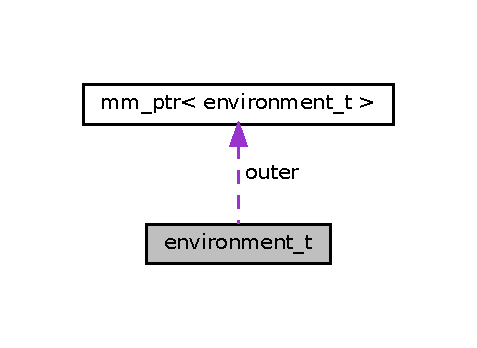
\includegraphics[width=229pt]{classenvironment__t__coll__graph}
\end{center}
\end{figure}
\subsection*{Открытые члены}
\begin{DoxyCompactItemize}
\item 
\mbox{\Hypertarget{classenvironment__t_ae631097efee20f081155ff042846e78a}\label{classenvironment__t_ae631097efee20f081155ff042846e78a}} 
{\bfseries environment\+\_\+t} (const \mbox{\hyperlink{classmm__ptr}{env\+\_\+ptr}} \&env)
\item 
\mbox{\Hypertarget{classenvironment__t_a5fd6c05d0a06a1a8e11e55488a171c92}\label{classenvironment__t_a5fd6c05d0a06a1a8e11e55488a171c92}} 
\mbox{\hyperlink{classenvironment__t}{environment\+\_\+t}} \& {\bfseries operator=} (const \mbox{\hyperlink{classenvironment__t}{environment\+\_\+t}} \&env)
\item 
\mbox{\Hypertarget{classenvironment__t_a7c7e79b474187b68cb00105b1ab40483}\label{classenvironment__t_a7c7e79b474187b68cb00105b1ab40483}} 
bool {\bfseries operator==} (const \mbox{\hyperlink{classenvironment__t}{environment\+\_\+t}} \&other)
\item 
\mbox{\Hypertarget{classenvironment__t_a09bf874d308fe51efbcc1632cc8e7b4e}\label{classenvironment__t_a09bf874d308fe51efbcc1632cc8e7b4e}} 
\mbox{\hyperlink{dict__t_8hpp_a56fdc8959ea1ff56de0242f602b1e649}{dict\+\_\+t}} {\bfseries get\+\_\+symbols} ()
\item 
void \mbox{\hyperlink{classenvironment__t_ac45c20ebf992a8288b2f3fc80cc4ec7e}{add\+\_\+symbols}} (const std\+::map$<$ const char $\ast$, std\+::pair$<$ function\+\_\+t, size\+\_\+t $>$$>$ \&)
\begin{DoxyCompactList}\small\item\em Добавляет символы из таблицы символов \end{DoxyCompactList}\item 
\mbox{\hyperlink{classmm__ptr}{obj\+\_\+ptr}} \mbox{\hyperlink{classenvironment__t_a29d163ecd74f5fae6a0ac5614d580387}{find}} (\mbox{\hyperlink{lisp__types_8hpp_a543c62d3ca4ba3750602b9c6b11af1de}{symbol\+\_\+t}} \&)
\begin{DoxyCompactList}\small\item\em Функция поиска символа в окружении \end{DoxyCompactList}\item 
void \mbox{\hyperlink{classenvironment__t_a5186921234c3252294cbd37e6616dc26}{define}} (\mbox{\hyperlink{lisp__types_8hpp_a543c62d3ca4ba3750602b9c6b11af1de}{symbol\+\_\+t}} \&, \mbox{\hyperlink{classmm__ptr}{obj\+\_\+ptr}})
\begin{DoxyCompactList}\small\item\em Создает новый символ в окружении \end{DoxyCompactList}\item 
bool \mbox{\hyperlink{classenvironment__t_a73cbdbc4b02e7efd863b5d4cbc3bc6c8}{change}} (\mbox{\hyperlink{lisp__types_8hpp_a543c62d3ca4ba3750602b9c6b11af1de}{symbol\+\_\+t}} \&, \mbox{\hyperlink{classmm__ptr}{obj\+\_\+ptr}})
\begin{DoxyCompactList}\small\item\em Изменяет значение уже существующего символа \end{DoxyCompactList}\item 
\mbox{\hyperlink{classmm__ptr}{env\+\_\+ptr}} \mbox{\hyperlink{classenvironment__t_a2b3db01d40e9b94f8234252768a5a396}{append}} (\mbox{\hyperlink{classmm__ptr}{env\+\_\+ptr}})
\begin{DoxyCompactList}\small\item\em Прицеляет окружение в конец переданной цепочки окружений \end{DoxyCompactList}\item 
\mbox{\Hypertarget{classenvironment__t_af007eec97ac909cbb8c2e9cc2b94c436}\label{classenvironment__t_af007eec97ac909cbb8c2e9cc2b94c436}} 
bool {\bfseries is\+\_\+global} ()
\end{DoxyCompactItemize}
\subsection*{Открытые атрибуты}
\begin{DoxyCompactItemize}
\item 
\mbox{\Hypertarget{classenvironment__t_af987f6d3a0b7ab1ab2c488541aa6f6c9}\label{classenvironment__t_af987f6d3a0b7ab1ab2c488541aa6f6c9}} 
\mbox{\hyperlink{classmm__ptr}{env\+\_\+ptr}} {\bfseries outer}
\end{DoxyCompactItemize}


\subsection{Подробное описание}
Класс lisp-\/типа окружения 

Данный класс отвечает за представление окружений, которые хранят таблицы символов связанных с значениями (процедурами) 

\subsection{Методы}
\mbox{\Hypertarget{classenvironment__t_ac45c20ebf992a8288b2f3fc80cc4ec7e}\label{classenvironment__t_ac45c20ebf992a8288b2f3fc80cc4ec7e}} 
\index{environment\+\_\+t@{environment\+\_\+t}!add\+\_\+symbols@{add\+\_\+symbols}}
\index{add\+\_\+symbols@{add\+\_\+symbols}!environment\+\_\+t@{environment\+\_\+t}}
\subsubsection{\texorpdfstring{add\+\_\+symbols()}{add\_symbols()}}
{\footnotesize\ttfamily void environment\+\_\+t\+::add\+\_\+symbols (\begin{DoxyParamCaption}\item[{const std\+::map$<$ const char $\ast$, std\+::pair$<$ function\+\_\+t, size\+\_\+t $>$$>$ \&}]{ }\end{DoxyParamCaption})}



Добавляет символы из таблицы символов 

Таблицы символов используются для описания интерфейса библиотек \mbox{\Hypertarget{classenvironment__t_a2b3db01d40e9b94f8234252768a5a396}\label{classenvironment__t_a2b3db01d40e9b94f8234252768a5a396}} 
\index{environment\+\_\+t@{environment\+\_\+t}!append@{append}}
\index{append@{append}!environment\+\_\+t@{environment\+\_\+t}}
\subsubsection{\texorpdfstring{append()}{append()}}
{\footnotesize\ttfamily \mbox{\hyperlink{classmm__ptr}{env\+\_\+ptr}} environment\+\_\+t\+::append (\begin{DoxyParamCaption}\item[{\mbox{\hyperlink{classmm__ptr}{env\+\_\+ptr}}}]{other }\end{DoxyParamCaption})}



Прицеляет окружение в конец переданной цепочки окружений 


\begin{DoxyParams}{Аргументы}
{\em other} & Окружение которое необходимо прицепить \\
\hline
\end{DoxyParams}
\begin{DoxyReturn}{Возвращает}
Указатель на окружение к которому было прицеплено окружение {\itshape other} 
\end{DoxyReturn}
\mbox{\Hypertarget{classenvironment__t_a73cbdbc4b02e7efd863b5d4cbc3bc6c8}\label{classenvironment__t_a73cbdbc4b02e7efd863b5d4cbc3bc6c8}} 
\index{environment\+\_\+t@{environment\+\_\+t}!change@{change}}
\index{change@{change}!environment\+\_\+t@{environment\+\_\+t}}
\subsubsection{\texorpdfstring{change()}{change()}}
{\footnotesize\ttfamily bool environment\+\_\+t\+::change (\begin{DoxyParamCaption}\item[{\mbox{\hyperlink{lisp__types_8hpp_a543c62d3ca4ba3750602b9c6b11af1de}{symbol\+\_\+t}} \&}]{symbol,  }\item[{\mbox{\hyperlink{classmm__ptr}{obj\+\_\+ptr}}}]{exp }\end{DoxyParamCaption})}



Изменяет значение уже существующего символа 


\begin{DoxyParams}{Аргументы}
{\em symbol} & Символ значение которого необходимо изменить \\
\hline
{\em exp} & Новое значение символа \\
\hline
\end{DoxyParams}
\begin{DoxyReturn}{Возвращает}
true, если значение символа было удачно изменено иначе false 
\end{DoxyReturn}
\mbox{\Hypertarget{classenvironment__t_a5186921234c3252294cbd37e6616dc26}\label{classenvironment__t_a5186921234c3252294cbd37e6616dc26}} 
\index{environment\+\_\+t@{environment\+\_\+t}!define@{define}}
\index{define@{define}!environment\+\_\+t@{environment\+\_\+t}}
\subsubsection{\texorpdfstring{define()}{define()}}
{\footnotesize\ttfamily void environment\+\_\+t\+::define (\begin{DoxyParamCaption}\item[{\mbox{\hyperlink{lisp__types_8hpp_a543c62d3ca4ba3750602b9c6b11af1de}{symbol\+\_\+t}} \&}]{symbol,  }\item[{\mbox{\hyperlink{classmm__ptr}{obj\+\_\+ptr}}}]{exp }\end{DoxyParamCaption})}



Создает новый символ в окружении 


\begin{DoxyParams}{Аргументы}
{\em symbol} & Символ для определения \\
\hline
{\em exp} & Значение символа \\
\hline
\end{DoxyParams}
\mbox{\Hypertarget{classenvironment__t_a29d163ecd74f5fae6a0ac5614d580387}\label{classenvironment__t_a29d163ecd74f5fae6a0ac5614d580387}} 
\index{environment\+\_\+t@{environment\+\_\+t}!find@{find}}
\index{find@{find}!environment\+\_\+t@{environment\+\_\+t}}
\subsubsection{\texorpdfstring{find()}{find()}}
{\footnotesize\ttfamily \mbox{\hyperlink{classmm__ptr}{obj\+\_\+ptr}} environment\+\_\+t\+::find (\begin{DoxyParamCaption}\item[{\mbox{\hyperlink{lisp__types_8hpp_a543c62d3ca4ba3750602b9c6b11af1de}{symbol\+\_\+t}} \&}]{symbol }\end{DoxyParamCaption})}



Функция поиска символа в окружении 


\begin{DoxyParams}{Аргументы}
{\em symbol} & Ссылка на искомый символ \\
\hline
\end{DoxyParams}
\begin{DoxyReturn}{Возвращает}
Либо ссылку на объект -\/ значение символа, либо указатель на пустой объект 
\end{DoxyReturn}


Объявления и описания членов классов находятся в файлах\+:\begin{DoxyCompactItemize}
\item 
/home/pablo/\+Net\+Beans\+Projects/d\+Lisp/types/\mbox{\hyperlink{environment__t_8hpp}{environment\+\_\+t.\+hpp}}\item 
/home/pablo/\+Net\+Beans\+Projects/d\+Lisp/environment\+\_\+t.\+cpp\end{DoxyCompactItemize}

\hypertarget{classlisp__error}{}\section{Класс lisp\+\_\+error}
\label{classlisp__error}\index{lisp\+\_\+error@{lisp\+\_\+error}}


Граф наследования\+:lisp\+\_\+error\+:\nopagebreak
\begin{figure}[H]
\begin{center}
\leavevmode
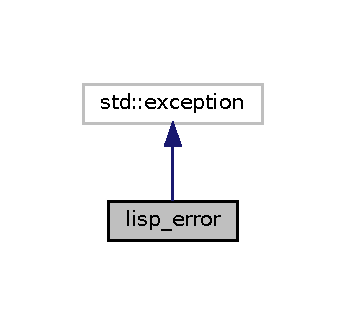
\includegraphics[width=166pt]{classlisp__error__inherit__graph}
\end{center}
\end{figure}


Граф связей класса lisp\+\_\+error\+:\nopagebreak
\begin{figure}[H]
\begin{center}
\leavevmode
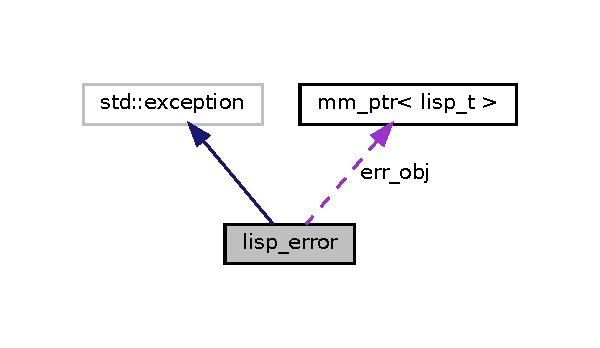
\includegraphics[width=288pt]{classlisp__error__coll__graph}
\end{center}
\end{figure}
\subsection*{Открытые члены}
\begin{DoxyCompactItemize}
\item 
\mbox{\Hypertarget{classlisp__error_ae41aa8025571dc7a8fb3686e20909978}\label{classlisp__error_ae41aa8025571dc7a8fb3686e20909978}} 
{\bfseries lisp\+\_\+error} (std\+::string \&\&str)
\item 
\mbox{\Hypertarget{classlisp__error_a28cdca7ae82bdb51add8f3ee176a7670}\label{classlisp__error_a28cdca7ae82bdb51add8f3ee176a7670}} 
{\bfseries lisp\+\_\+error} (std\+::string \&\&str, \mbox{\hyperlink{classmm__ptr}{obj\+\_\+ptr}} obj)
\item 
\mbox{\Hypertarget{classlisp__error_a3ef4f940064ddba3557fd8fe5cd74399}\label{classlisp__error_a3ef4f940064ddba3557fd8fe5cd74399}} 
const char $\ast$ {\bfseries what} () const noexcept
\end{DoxyCompactItemize}
\subsection*{Открытые атрибуты}
\begin{DoxyCompactItemize}
\item 
\mbox{\Hypertarget{classlisp__error_a7bd15a33b45c21b4329efae8c233d3e2}\label{classlisp__error_a7bd15a33b45c21b4329efae8c233d3e2}} 
std\+::string {\bfseries err\+\_\+str}
\item 
\mbox{\Hypertarget{classlisp__error_aa6ffa1f360005d7d4776c05466a79042}\label{classlisp__error_aa6ffa1f360005d7d4776c05466a79042}} 
\mbox{\hyperlink{classmm__ptr}{obj\+\_\+ptr}} {\bfseries err\+\_\+obj}
\item 
\mbox{\Hypertarget{classlisp__error_af91e2e580c735dca963cc27bfc3addad}\label{classlisp__error_af91e2e580c735dca963cc27bfc3addad}} 
bool {\bfseries add\+\_\+proc} = false
\end{DoxyCompactItemize}


Объявления и описания членов класса находятся в файле\+:\begin{DoxyCompactItemize}
\item 
/home/pablo/\+Net\+Beans\+Projects/d\+Lisp/exceptions.\+hpp\end{DoxyCompactItemize}

\hypertarget{structlisp__t}{}\section{Структура lisp\+\_\+t}
\label{structlisp__t}\index{lisp\+\_\+t@{lisp\+\_\+t}}


Граф связей класса lisp\+\_\+t\+:
\nopagebreak
\begin{figure}[H]
\begin{center}
\leavevmode
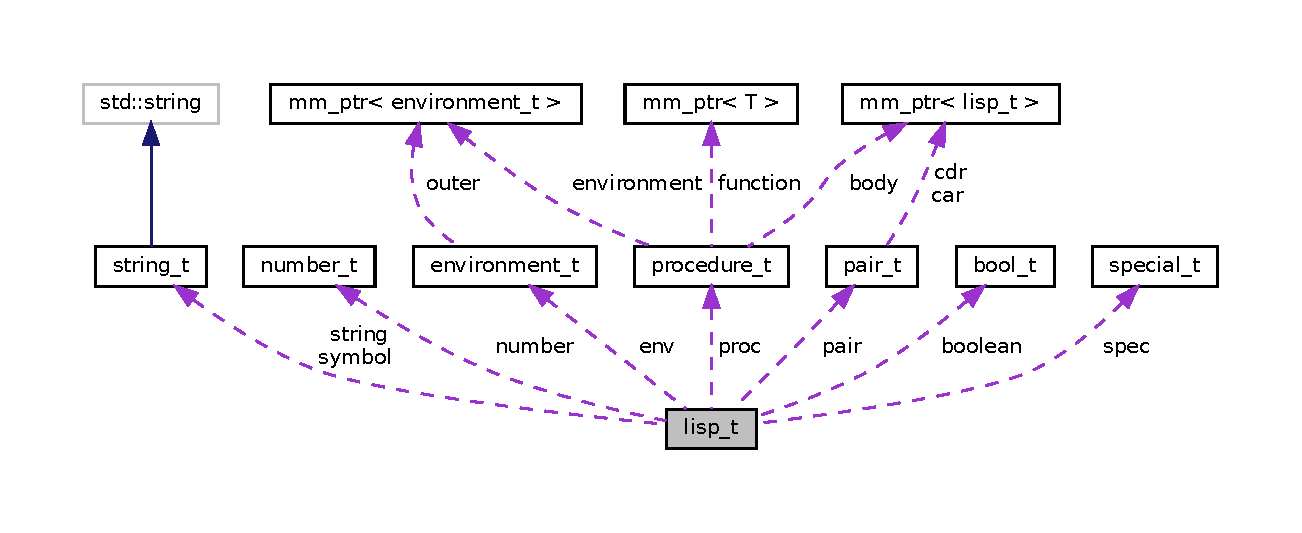
\includegraphics[width=350pt]{structlisp__t__coll__graph}
\end{center}
\end{figure}
\subsection*{Открытые члены}
\begin{DoxyCompactItemize}
\item 
\mbox{\Hypertarget{structlisp__t_a8440291143a1d2e77211729d991f5488}\label{structlisp__t_a8440291143a1d2e77211729d991f5488}} 
{\bfseries lisp\+\_\+t} (\mbox{\hyperlink{lisp__type__flag_8hpp_a055b7e4c72b7a614806ae1225539b99f}{lisp\+\_\+type\+\_\+flag}} type)
\item 
\mbox{\Hypertarget{structlisp__t_a905f36e0f3f94843189a0dcb863b751e}\label{structlisp__t_a905f36e0f3f94843189a0dcb863b751e}} 
{\footnotesize template$<$class T $>$ }\\{\bfseries lisp\+\_\+t} (\mbox{\hyperlink{lisp__type__flag_8hpp_a055b7e4c72b7a614806ae1225539b99f}{lisp\+\_\+type\+\_\+flag}} type, const T \&value)
\item 
\mbox{\Hypertarget{structlisp__t_aa591bc4bd65be7cd9377f3a33abb9259}\label{structlisp__t_aa591bc4bd65be7cd9377f3a33abb9259}} 
bool {\bfseries operator==} (const \mbox{\hyperlink{structlisp__t}{lisp\+\_\+t}} \&)
\item 
\mbox{\Hypertarget{structlisp__t_a3148073588fe6aa2bb6a0704e4ed1f21}\label{structlisp__t_a3148073588fe6aa2bb6a0704e4ed1f21}} 
\mbox{\hyperlink{structlisp__t}{lisp\+\_\+t}} \& {\bfseries operator=} (const \mbox{\hyperlink{structlisp__t}{lisp\+\_\+t}} \&)
\item 
\mbox{\Hypertarget{structlisp__t_a4dcb779c9e6f4188182c10212d4d7bd5}\label{structlisp__t_a4dcb779c9e6f4188182c10212d4d7bd5}} 
void {\bfseries append} (\mbox{\hyperlink{classmm__ptr}{obj\+\_\+ptr}})
\item 
\mbox{\Hypertarget{structlisp__t_a23ae5189d44aa8845528a7d743e9c54f}\label{structlisp__t_a23ae5189d44aa8845528a7d743e9c54f}} 
size\+\_\+t {\bfseries len} ()
\item 
\mbox{\Hypertarget{structlisp__t_adf2f843efc9dacb5400650b885e24510}\label{structlisp__t_adf2f843efc9dacb5400650b885e24510}} 
\mbox{\hyperlink{classmm__ptr}{obj\+\_\+ptr}} {\bfseries at} (size\+\_\+t)
\item 
\mbox{\Hypertarget{structlisp__t_ad4f1105bd90db1aab9e80e73a359758f}\label{structlisp__t_ad4f1105bd90db1aab9e80e73a359758f}} 
\mbox{\hyperlink{classmm__ptr}{obj\+\_\+ptr}} {\bfseries end} ()
\item 
\mbox{\Hypertarget{structlisp__t_a24e25c442fa9728a7a6f3fbbe0f0b7ac}\label{structlisp__t_a24e25c442fa9728a7a6f3fbbe0f0b7ac}} 
bool {\bfseries is\+\_\+atom} ()
\item 
\mbox{\Hypertarget{structlisp__t_a3e5c43cf5de9bfbd4f65e85384553da4}\label{structlisp__t_a3e5c43cf5de9bfbd4f65e85384553da4}} 
bool {\bfseries is\+\_\+self\+\_\+evaluating} ()
\item 
\mbox{\Hypertarget{structlisp__t_afe1a04de73d94cdc3464c57015943885}\label{structlisp__t_afe1a04de73d94cdc3464c57015943885}} 
bool {\bfseries is\+\_\+true} ()
\item 
\mbox{\Hypertarget{structlisp__t_a1e7e3371571d50cd5704833db1520b46}\label{structlisp__t_a1e7e3371571d50cd5704833db1520b46}} 
bool {\bfseries is\+\_\+null} ()
\item 
\mbox{\Hypertarget{structlisp__t_ac991f97b3c78b0831bab87b78c81caf3}\label{structlisp__t_ac991f97b3c78b0831bab87b78c81caf3}} 
bool {\bfseries is\+\_\+list} ()
\item 
\mbox{\Hypertarget{structlisp__t_a2bc45fdc33116b2bfd96d16ca3c2e444}\label{structlisp__t_a2bc45fdc33116b2bfd96d16ca3c2e444}} 
bool {\bfseries is\+\_\+pair} ()
\item 
\mbox{\Hypertarget{structlisp__t_ab91960538f83af8e2967f7b4e373a18a}\label{structlisp__t_ab91960538f83af8e2967f7b4e373a18a}} 
bool {\bfseries is\+\_\+pair\+\_\+syntax} ()
\item 
\mbox{\Hypertarget{structlisp__t_ae954f28ed86c5a16cc5962d7fac0b930}\label{structlisp__t_ae954f28ed86c5a16cc5962d7fac0b930}} 
{\footnotesize template$<$$>$ }\\{\bfseries lisp\+\_\+t} (\mbox{\hyperlink{lisp__type__flag_8hpp_a055b7e4c72b7a614806ae1225539b99f}{lisp\+\_\+type\+\_\+flag}} type, const \mbox{\hyperlink{classprocedure__t}{procedure\+\_\+t}} \&value)
\item 
\mbox{\Hypertarget{structlisp__t_a7f359f30c0ceabb9c53350992549b312}\label{structlisp__t_a7f359f30c0ceabb9c53350992549b312}} 
{\footnotesize template$<$$>$ }\\{\bfseries lisp\+\_\+t} (\mbox{\hyperlink{lisp__type__flag_8hpp_a055b7e4c72b7a614806ae1225539b99f}{lisp\+\_\+type\+\_\+flag}} type, const \mbox{\hyperlink{classenvironment__t}{environment\+\_\+t}} \&value)
\end{DoxyCompactItemize}
\subsection*{Открытые атрибуты}
\begin{DoxyCompactItemize}
\item 
\mbox{\Hypertarget{structlisp__t_af4d31fea3ded5de3f14b57a6eb9f996c}\label{structlisp__t_af4d31fea3ded5de3f14b57a6eb9f996c}} 
\mbox{\hyperlink{lisp__type__flag_8hpp_a055b7e4c72b7a614806ae1225539b99f}{lisp\+\_\+type\+\_\+flag}} {\bfseries type}
\item 
\mbox{\Hypertarget{structlisp__t_a466003f82a1bafc2c3c743266fe5ab47}\label{structlisp__t_a466003f82a1bafc2c3c743266fe5ab47}} 
\begin{tabbing}
xx\=xx\=xx\=xx\=xx\=xx\=xx\=xx\=xx\=\kill
union \{\\
\>\mbox{\hyperlink{classnumber__t}{number\_t}} {\bfseries number}\\
\>\mbox{\hyperlink{classstring__t}{string\_t}} {\bfseries string}\\
\>\mbox{\hyperlink{lisp__types_8hpp_a543c62d3ca4ba3750602b9c6b11af1de}{symbol\_t}} {\bfseries symbol}\\
\>\mbox{\hyperlink{classprocedure__t}{procedure\_t}} {\bfseries proc}\\
\>\mbox{\hyperlink{classpair__t}{pair\_t}} {\bfseries pair}\\
\>\mbox{\hyperlink{classbool__t}{bool\_t}} {\bfseries boolean}\\
\>\mbox{\hyperlink{classspecial__t}{special\_t}} {\bfseries spec}\\
\>\mbox{\hyperlink{classenvironment__t}{environment\_t}} {\bfseries env}\\
\}; \\

\end{tabbing}\end{DoxyCompactItemize}


Объявления и описания членов структур находятся в файлах\+:\begin{DoxyCompactItemize}
\item 
/home/pablo/\+Net\+Beans\+Projects/d\+Lisp/types/lisp\+\_\+t.\+hpp\item 
/home/pablo/\+Net\+Beans\+Projects/d\+Lisp/lisp\+\_\+t.\+cpp\end{DoxyCompactItemize}

\hypertarget{classmemory__manager}{}\section{Класс memory\+\_\+manager}
\label{classmemory__manager}\index{memory\+\_\+manager@{memory\+\_\+manager}}
\subsection*{Открытые члены}
\begin{DoxyCompactItemize}
\item 
\mbox{\Hypertarget{classmemory__manager_a05c8cf8b2eb3d8411f70acec0f2c1d15}\label{classmemory__manager_a05c8cf8b2eb3d8411f70acec0f2c1d15}} 
index\+\_\+t {\bfseries allocate\+\_\+object} (const \mbox{\hyperlink{structlisp__t}{lisp\+\_\+t}} \&)
\item 
\mbox{\Hypertarget{classmemory__manager_a1da18ca2fca10dbac0f4ce98a697dc91}\label{classmemory__manager_a1da18ca2fca10dbac0f4ce98a697dc91}} 
\mbox{\hyperlink{structlisp__t}{lisp\+\_\+t}} $\ast$ {\bfseries get\+\_\+object} (index\+\_\+t)
\item 
\mbox{\Hypertarget{classmemory__manager_a224b6bf9b6302d6ff08855531dc06be5}\label{classmemory__manager_a224b6bf9b6302d6ff08855531dc06be5}} 
index\+\_\+t {\bfseries get\+\_\+index} (\mbox{\hyperlink{structlisp__t}{lisp\+\_\+t}} $\ast$obj)
\item 
\mbox{\Hypertarget{classmemory__manager_a106e0194f6016f5a9ff2953d16788cf3}\label{classmemory__manager_a106e0194f6016f5a9ff2953d16788cf3}} 
index\+\_\+t {\bfseries next\+\_\+index} ()
\item 
\mbox{\Hypertarget{classmemory__manager_ae7472b4732ee8eb2d4af1aec8b973ac0}\label{classmemory__manager_ae7472b4732ee8eb2d4af1aec8b973ac0}} 
void $\ast$ {\bfseries find\+\_\+or\+\_\+add\+\_\+cell} (void $\ast$, size\+\_\+t)
\item 
\mbox{\Hypertarget{classmemory__manager_a616639b8ece6314ea8f9cbd5e3ff3dd0}\label{classmemory__manager_a616639b8ece6314ea8f9cbd5e3ff3dd0}} 
int {\bfseries check\+\_\+memory\+\_\+use} ()
\item 
\mbox{\Hypertarget{classmemory__manager_ae054893d75db7f5042bc2401f06ee2e9}\label{classmemory__manager_ae054893d75db7f5042bc2401f06ee2e9}} 
int {\bfseries cells\+\_\+count} ()
\item 
\mbox{\Hypertarget{classmemory__manager_a4fced86e5194cad808f70806d7b05417}\label{classmemory__manager_a4fced86e5194cad808f70806d7b05417}} 
int {\bfseries free\+\_\+cells\+\_\+count} ()
\end{DoxyCompactItemize}


Объявления и описания членов классов находятся в файлах\+:\begin{DoxyCompactItemize}
\item 
/home/pablo/\+Net\+Beans\+Projects/d\+Lisp/memory\+\_\+manager.\+hpp\item 
/home/pablo/\+Net\+Beans\+Projects/d\+Lisp/memory\+\_\+manager.\+cpp\end{DoxyCompactItemize}

\hypertarget{classmm__ptr}{}\section{Шаблон класса mm\+\_\+ptr$<$ T $>$}
\label{classmm__ptr}\index{mm\+\_\+ptr$<$ T $>$@{mm\+\_\+ptr$<$ T $>$}}
\subsection*{Открытые члены}
\begin{DoxyCompactItemize}
\item 
\mbox{\Hypertarget{classmm__ptr_aa3b923c8263b7be8549cbe6bc8a5c98c}\label{classmm__ptr_aa3b923c8263b7be8549cbe6bc8a5c98c}} 
{\bfseries mm\+\_\+ptr} (index\+\_\+t obj)
\item 
\mbox{\Hypertarget{classmm__ptr_aa3b08f2a7e216e1592bf32a003e310cd}\label{classmm__ptr_aa3b08f2a7e216e1592bf32a003e310cd}} 
{\bfseries mm\+\_\+ptr} (const \mbox{\hyperlink{classmm__ptr}{mm\+\_\+ptr}} \&m)
\item 
\mbox{\Hypertarget{classmm__ptr_aeaa092d03f5ddcf1be1b8f34479b086e}\label{classmm__ptr_aeaa092d03f5ddcf1be1b8f34479b086e}} 
bool {\bfseries operator==} (const \mbox{\hyperlink{classmm__ptr}{mm\+\_\+ptr}}$<$ T $>$ \&other)
\item 
\mbox{\Hypertarget{classmm__ptr_a7ffa5b886182413a429bfab972a27653}\label{classmm__ptr_a7ffa5b886182413a429bfab972a27653}} 
bool {\bfseries operator!=} (const \mbox{\hyperlink{classmm__ptr}{mm\+\_\+ptr}}$<$ T $>$ \&other)
\item 
\mbox{\Hypertarget{classmm__ptr_ab0954ffa5e2b0989df25061dc2ab1df4}\label{classmm__ptr_ab0954ffa5e2b0989df25061dc2ab1df4}} 
{\footnotesize template$<$class T2 $>$ }\\T2 {\bfseries as\+\_\+type} ()
\item 
\mbox{\Hypertarget{classmm__ptr_a8507bb1d8946b075bbb34ae4570efc9a}\label{classmm__ptr_a8507bb1d8946b075bbb34ae4570efc9a}} 
T $\ast$ {\bfseries operator-\/$>$} ()
\item 
\mbox{\Hypertarget{classmm__ptr_a62fce96ab6c4c1073c97ddaec8dac83f}\label{classmm__ptr_a62fce96ab6c4c1073c97ddaec8dac83f}} 
T \& {\bfseries operator$\ast$} ()
\item 
\mbox{\Hypertarget{classmm__ptr_a9872d528e7c8a788acd02ccae0c9069c}\label{classmm__ptr_a9872d528e7c8a788acd02ccae0c9069c}} 
{\bfseries operator T$\ast$} ()
\item 
\mbox{\Hypertarget{classmm__ptr_a14de2f1e2d597acfa6e145238da2920d}\label{classmm__ptr_a14de2f1e2d597acfa6e145238da2920d}} 
bool {\bfseries is\+\_\+null} ()
\end{DoxyCompactItemize}


Объявления и описания членов класса находятся в файле\+:\begin{DoxyCompactItemize}
\item 
/home/pablo/\+Net\+Beans\+Projects/d\+Lisp/mm\+\_\+ptr.\+hpp\end{DoxyCompactItemize}

\hypertarget{classnumber__t}{}\section{Класс number\+\_\+t}
\label{classnumber__t}\index{number\+\_\+t@{number\+\_\+t}}


Класс lisp-\/типа чисел  




{\ttfamily \#include $<$number\+\_\+t.\+hpp$>$}

\subsection*{Открытые члены}
\begin{DoxyCompactItemize}
\item 
\mbox{\Hypertarget{classnumber__t_a62c293bbf71ab10867cc6eb4f9cfced4}\label{classnumber__t_a62c293bbf71ab10867cc6eb4f9cfced4}} 
{\bfseries number\+\_\+t} (\mbox{\hyperlink{number__t_8hpp_a9c37ed0386636f462116b6e8d1fd8312}{number\+\_\+type\+\_\+flag}} type, long double num)
\item 
\mbox{\Hypertarget{classnumber__t_a7937289aec5501024cf903613f04192b}\label{classnumber__t_a7937289aec5501024cf903613f04192b}} 
{\bfseries number\+\_\+t} (long double num)
\item 
\mbox{\Hypertarget{classnumber__t_aac9b03b1c5596ed3f95d4a4ba878b110}\label{classnumber__t_aac9b03b1c5596ed3f95d4a4ba878b110}} 
void \mbox{\hyperlink{classnumber__t_aac9b03b1c5596ed3f95d4a4ba878b110}{raise\+\_\+type}} ()
\begin{DoxyCompactList}\small\item\em Уточнение типа числа \end{DoxyCompactList}\item 
\mbox{\Hypertarget{classnumber__t_ad6f4eea4d15cd960db85d864895d4099}\label{classnumber__t_ad6f4eea4d15cd960db85d864895d4099}} 
bool {\bfseries operator==} (const \mbox{\hyperlink{classnumber__t}{number\+\_\+t}} \&other)
\item 
\mbox{\Hypertarget{classnumber__t_a57715f62c21357737396f71b9a45aa99}\label{classnumber__t_a57715f62c21357737396f71b9a45aa99}} 
bool {\bfseries operator$<$} (const \mbox{\hyperlink{classnumber__t}{number\+\_\+t}} \&other)
\item 
\mbox{\Hypertarget{classnumber__t_a30028f85921ce59a6163378f4ca52182}\label{classnumber__t_a30028f85921ce59a6163378f4ca52182}} 
bool {\bfseries operator$>$} (const \mbox{\hyperlink{classnumber__t}{number\+\_\+t}} \&other)
\item 
\mbox{\Hypertarget{classnumber__t_ab23509dad5bfadd4f0ec1087edb0cfcf}\label{classnumber__t_ab23509dad5bfadd4f0ec1087edb0cfcf}} 
bool {\bfseries operator$<$=} (const \mbox{\hyperlink{classnumber__t}{number\+\_\+t}} \&other)
\item 
\mbox{\Hypertarget{classnumber__t_ad0c004c476a1957cf7b1739da2b3f2ab}\label{classnumber__t_ad0c004c476a1957cf7b1739da2b3f2ab}} 
bool {\bfseries operator$>$=} (const \mbox{\hyperlink{classnumber__t}{number\+\_\+t}} \&other)
\item 
\mbox{\Hypertarget{classnumber__t_ad4a3796b50ebfe92f431ee775aa9f6b1}\label{classnumber__t_ad4a3796b50ebfe92f431ee775aa9f6b1}} 
\mbox{\hyperlink{classnumber__t}{number\+\_\+t}} {\bfseries operator+} (const \mbox{\hyperlink{classnumber__t}{number\+\_\+t}} \&other)
\item 
\mbox{\Hypertarget{classnumber__t_ae84652c43ac0276ab8dc4d81159d0982}\label{classnumber__t_ae84652c43ac0276ab8dc4d81159d0982}} 
\mbox{\hyperlink{classnumber__t}{number\+\_\+t}} {\bfseries operator-\/} (const \mbox{\hyperlink{classnumber__t}{number\+\_\+t}} \&other)
\item 
\mbox{\Hypertarget{classnumber__t_af23fecdd6694e7fc01de19ac15733854}\label{classnumber__t_af23fecdd6694e7fc01de19ac15733854}} 
\mbox{\hyperlink{classnumber__t}{number\+\_\+t}} {\bfseries operator$\ast$} (const \mbox{\hyperlink{classnumber__t}{number\+\_\+t}} \&other)
\item 
\mbox{\Hypertarget{classnumber__t_aa475e09b8b3131516ba22aff5c00683f}\label{classnumber__t_aa475e09b8b3131516ba22aff5c00683f}} 
\mbox{\hyperlink{classnumber__t}{number\+\_\+t}} {\bfseries operator/} (const \mbox{\hyperlink{classnumber__t}{number\+\_\+t}} \&other)
\item 
\mbox{\Hypertarget{classnumber__t_a081a6ca6cd71e2481165fc96c865264a}\label{classnumber__t_a081a6ca6cd71e2481165fc96c865264a}} 
\mbox{\hyperlink{classnumber__t}{number\+\_\+t}} {\bfseries operator\%} (const \mbox{\hyperlink{classnumber__t}{number\+\_\+t}} \&other)
\item 
\mbox{\Hypertarget{classnumber__t_a1835d01c8fb573827545069b9a587dd8}\label{classnumber__t_a1835d01c8fb573827545069b9a587dd8}} 
\mbox{\hyperlink{classnumber__t}{number\+\_\+t}} \mbox{\hyperlink{classnumber__t_a1835d01c8fb573827545069b9a587dd8}{div}} (const \mbox{\hyperlink{classnumber__t}{number\+\_\+t}} \&other)
\begin{DoxyCompactList}\small\item\em Целочисленное деление чисел \end{DoxyCompactList}\end{DoxyCompactItemize}
\subsection*{Открытые атрибуты}
\begin{DoxyCompactItemize}
\item 
\mbox{\Hypertarget{classnumber__t_ab8105972a213fef8d6a25613f67447bd}\label{classnumber__t_ab8105972a213fef8d6a25613f67447bd}} 
\mbox{\hyperlink{number__t_8hpp_a9c37ed0386636f462116b6e8d1fd8312}{number\+\_\+type\+\_\+flag}} {\bfseries type}
\item 
\mbox{\Hypertarget{classnumber__t_a1ff6668c69c1642df4a2200ee9a87184}\label{classnumber__t_a1ff6668c69c1642df4a2200ee9a87184}} 
long double {\bfseries value}
\end{DoxyCompactItemize}


\subsection{Подробное описание}
Класс lisp-\/типа чисел 

Данный класс определяет представление чисел внутри интерпретатора и определяет основные операции для них. 

Объявления и описания членов классов находятся в файлах\+:\begin{DoxyCompactItemize}
\item 
/home/pablo/\+Net\+Beans\+Projects/d\+Lisp/types/\mbox{\hyperlink{number__t_8hpp}{number\+\_\+t.\+hpp}}\item 
/home/pablo/\+Net\+Beans\+Projects/d\+Lisp/number\+\_\+t.\+cpp\end{DoxyCompactItemize}

\hypertarget{classpair__t}{}\section{Класс pair\+\_\+t}
\label{classpair__t}\index{pair\+\_\+t@{pair\+\_\+t}}


Класс lisp-\/типа пар  




{\ttfamily \#include $<$pair\+\_\+t.\+hpp$>$}



Граф связей класса pair\+\_\+t\+:\nopagebreak
\begin{figure}[H]
\begin{center}
\leavevmode
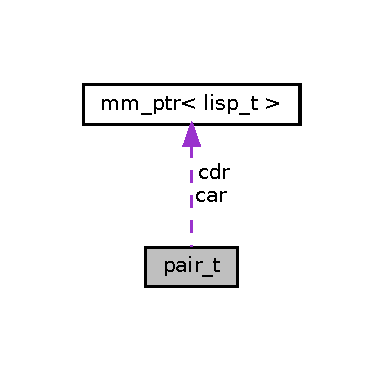
\includegraphics[width=184pt]{classpair__t__coll__graph}
\end{center}
\end{figure}
\subsection*{Открытые члены}
\begin{DoxyCompactItemize}
\item 
\mbox{\Hypertarget{classpair__t_adfa4aeb35f04b8d9efdd4e6d770feed9}\label{classpair__t_adfa4aeb35f04b8d9efdd4e6d770feed9}} 
{\bfseries pair\+\_\+t} (\mbox{\hyperlink{classmm__ptr}{obj\+\_\+ptr}} head, \mbox{\hyperlink{classmm__ptr}{obj\+\_\+ptr}} tail)
\end{DoxyCompactItemize}
\subsection*{Открытые атрибуты}
\begin{DoxyCompactItemize}
\item 
\mbox{\Hypertarget{classpair__t_a94511da44f476f4e3ec370939e9dfc3b}\label{classpair__t_a94511da44f476f4e3ec370939e9dfc3b}} 
\mbox{\hyperlink{classmm__ptr}{obj\+\_\+ptr}} {\bfseries car}
\item 
\mbox{\Hypertarget{classpair__t_a2064f2bd5085d7c589b56e76137ccf57}\label{classpair__t_a2064f2bd5085d7c589b56e76137ccf57}} 
\mbox{\hyperlink{classmm__ptr}{obj\+\_\+ptr}} {\bfseries cdr}
\end{DoxyCompactItemize}


\subsection{Подробное описание}
Класс lisp-\/типа пар 

Данный класс используется для представления пар и списков. 

Объявления и описания членов класса находятся в файле\+:\begin{DoxyCompactItemize}
\item 
/home/pablo/\+Net\+Beans\+Projects/d\+Lisp/types/\mbox{\hyperlink{pair__t_8hpp}{pair\+\_\+t.\+hpp}}\end{DoxyCompactItemize}

\hypertarget{classprocedure__t}{}\section{Класс procedure\+\_\+t}
\label{classprocedure__t}\index{procedure\+\_\+t@{procedure\+\_\+t}}


Класс lisp-\/типа процедуры  




{\ttfamily \#include $<$procedure\+\_\+t.\+hpp$>$}



Граф связей класса procedure\+\_\+t\+:\nopagebreak
\begin{figure}[H]
\begin{center}
\leavevmode
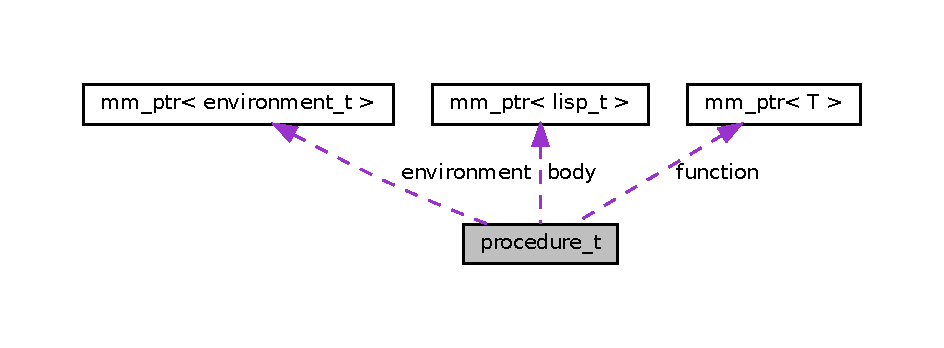
\includegraphics[width=350pt]{classprocedure__t__coll__graph}
\end{center}
\end{figure}
\subsection*{Открытые члены}
\begin{DoxyCompactItemize}
\item 
\mbox{\Hypertarget{classprocedure__t_a21d32b0db94eade1575ab4d7f7f8f73d}\label{classprocedure__t_a21d32b0db94eade1575ab4d7f7f8f73d}} 
{\bfseries procedure\+\_\+t} (function\+\_\+t f, size\+\_\+t c)
\item 
\mbox{\Hypertarget{classprocedure__t_ac2ecc9ec7167a96bbc8b1af2b4911a4a}\label{classprocedure__t_ac2ecc9ec7167a96bbc8b1af2b4911a4a}} 
\mbox{\hyperlink{classprocedure__t}{procedure\+\_\+t}} \& {\bfseries operator=} (const \mbox{\hyperlink{classprocedure__t}{procedure\+\_\+t}} \&)
\item 
\mbox{\Hypertarget{classprocedure__t_a9f765845f3c00f6bfdb6602fc7462d9e}\label{classprocedure__t_a9f765845f3c00f6bfdb6602fc7462d9e}} 
\mbox{\hyperlink{classmm__ptr}{obj\+\_\+ptr}} {\bfseries apply} (\mbox{\hyperlink{classmm__ptr}{obj\+\_\+ptr}}, \mbox{\hyperlink{classmm__ptr}{env\+\_\+ptr}})
\end{DoxyCompactItemize}
\subsection*{Открытые атрибуты}
\begin{DoxyCompactItemize}
\item 
\mbox{\Hypertarget{classprocedure__t_ae7b715b009091614021e87857ee497ad}\label{classprocedure__t_ae7b715b009091614021e87857ee497ad}} 
function\+\_\+t {\bfseries function} = nullptr
\item 
\mbox{\Hypertarget{classprocedure__t_a190e43c93a40ba4f11710ac6798b3e6a}\label{classprocedure__t_a190e43c93a40ba4f11710ac6798b3e6a}} 
size\+\_\+t {\bfseries argsc} = 0
\item 
\mbox{\Hypertarget{classprocedure__t_a0a30d3e1ff7fbb68dbe9bbc0b5feefd9}\label{classprocedure__t_a0a30d3e1ff7fbb68dbe9bbc0b5feefd9}} 
\mbox{\hyperlink{classmm__ptr}{obj\+\_\+ptr}} {\bfseries body}
\item 
\mbox{\Hypertarget{classprocedure__t_a0deef5a236964908f85b3da0300271f0}\label{classprocedure__t_a0deef5a236964908f85b3da0300271f0}} 
std\+::vector$<$ \mbox{\hyperlink{classmm__ptr}{obj\+\_\+ptr}} $>$ {\bfseries formal\+\_\+args}
\item 
\mbox{\Hypertarget{classprocedure__t_ab3c92a016be4b0b8ae25d9c705bfa61c}\label{classprocedure__t_ab3c92a016be4b0b8ae25d9c705bfa61c}} 
\mbox{\hyperlink{classmm__ptr}{env\+\_\+ptr}} {\bfseries environment}
\end{DoxyCompactItemize}


\subsection{Подробное описание}
Класс lisp-\/типа процедуры 

Данный класс предназначен для представления lisp-\/процедур, лямбда-\/фйнкций и замыканий 

Объявления и описания членов классов находятся в файлах\+:\begin{DoxyCompactItemize}
\item 
/home/pablo/\+Net\+Beans\+Projects/d\+Lisp/types/\mbox{\hyperlink{procedure__t_8hpp}{procedure\+\_\+t.\+hpp}}\item 
/home/pablo/\+Net\+Beans\+Projects/d\+Lisp/procedure\+\_\+t.\+cpp\end{DoxyCompactItemize}

\hypertarget{classspecial__t}{}\section{Класс special\+\_\+t}
\label{classspecial__t}\index{special\+\_\+t@{special\+\_\+t}}


Класс lisp-\/типа специальных значение  




{\ttfamily \#include $<$special\+\_\+t.\+hpp$>$}

\subsection*{Открытые члены}
\begin{DoxyCompactItemize}
\item 
\mbox{\Hypertarget{classspecial__t_aac3a593193f0196940190c54e9f6aa5c}\label{classspecial__t_aac3a593193f0196940190c54e9f6aa5c}} 
{\bfseries special\+\_\+t} (\mbox{\hyperlink{special__t_8hpp_af80c2ea5ebf91ef19f47fd2e190d7149}{special\+\_\+type\+\_\+flag}} type)
\item 
\mbox{\Hypertarget{classspecial__t_a42699488788fe74b3a0ca3969b6ba45a}\label{classspecial__t_a42699488788fe74b3a0ca3969b6ba45a}} 
{\bfseries special\+\_\+t} (const \mbox{\hyperlink{classspecial__t}{special\+\_\+t}} \&)
\item 
\mbox{\Hypertarget{classspecial__t_aad7430141412a11b5c40a61abd9297ab}\label{classspecial__t_aad7430141412a11b5c40a61abd9297ab}} 
bool {\bfseries operator==} (const \mbox{\hyperlink{classspecial__t}{special\+\_\+t}} \&other)
\end{DoxyCompactItemize}
\subsection*{Открытые атрибуты}
\begin{DoxyCompactItemize}
\item 
\mbox{\Hypertarget{classspecial__t_ae86baa19a7cb7796ee6cdd24c76836ac}\label{classspecial__t_ae86baa19a7cb7796ee6cdd24c76836ac}} 
\mbox{\hyperlink{special__t_8hpp_af80c2ea5ebf91ef19f47fd2e190d7149}{special\+\_\+type\+\_\+flag}} {\bfseries type}
\end{DoxyCompactItemize}


\subsection{Подробное описание}
Класс lisp-\/типа специальных значение 

Данный класс предназначен для предсталения специальных внутрених значений интерпретатора, которые не могут быть использованы в вычислениях напрямую 

Объявления и описания членов класса находятся в файле\+:\begin{DoxyCompactItemize}
\item 
/home/pablo/\+Net\+Beans\+Projects/d\+Lisp/types/\mbox{\hyperlink{special__t_8hpp}{special\+\_\+t.\+hpp}}\end{DoxyCompactItemize}

\hypertarget{classstring__t}{}\section{Класс string\+\_\+t}
\label{classstring__t}\index{string\+\_\+t@{string\+\_\+t}}


Класс lisp-\/типа строк  




{\ttfamily \#include $<$string\+\_\+t.\+hpp$>$}



Граф наследования\+:string\+\_\+t\+:\nopagebreak
\begin{figure}[H]
\begin{center}
\leavevmode
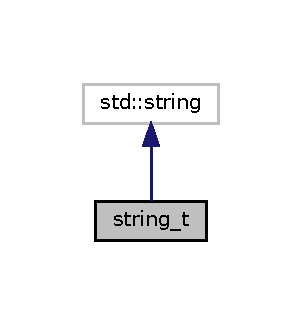
\includegraphics[width=145pt]{classstring__t__inherit__graph}
\end{center}
\end{figure}


Граф связей класса string\+\_\+t\+:\nopagebreak
\begin{figure}[H]
\begin{center}
\leavevmode
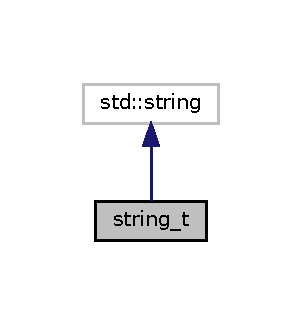
\includegraphics[width=145pt]{classstring__t__coll__graph}
\end{center}
\end{figure}
\subsection*{Открытые члены}
\begin{DoxyCompactItemize}
\item 
\mbox{\Hypertarget{classstring__t_ae45693d39bbe0865165ff3e8d3f9a523}\label{classstring__t_ae45693d39bbe0865165ff3e8d3f9a523}} 
{\bfseries string\+\_\+t} (std\+::string \&str)
\item 
\mbox{\Hypertarget{classstring__t_a3e35899571ea6d5a6f69f75650b09f4e}\label{classstring__t_a3e35899571ea6d5a6f69f75650b09f4e}} 
{\bfseries string\+\_\+t} (const char $\ast$str)
\end{DoxyCompactItemize}


\subsection{Подробное описание}
Класс lisp-\/типа строк 

Объявления и описания членов класса находятся в файле\+:\begin{DoxyCompactItemize}
\item 
/home/pablo/\+Net\+Beans\+Projects/d\+Lisp/types/\mbox{\hyperlink{string__t_8hpp}{string\+\_\+t.\+hpp}}\end{DoxyCompactItemize}

\hypertarget{structtoken}{}\section{Структура token}
\label{structtoken}\index{token@{token}}
\subsection*{Открытые члены}
\begin{DoxyCompactItemize}
\item 
\mbox{\Hypertarget{structtoken_aa87b4aa0605b95aaa5d5025a8b08c036}\label{structtoken_aa87b4aa0605b95aaa5d5025a8b08c036}} 
{\bfseries token} (token\+\_\+flag type, const char $\ast$str)
\end{DoxyCompactItemize}
\subsection*{Открытые атрибуты}
\begin{DoxyCompactItemize}
\item 
\mbox{\Hypertarget{structtoken_a1100177b59da20ffc298ada3d67c32e4}\label{structtoken_a1100177b59da20ffc298ada3d67c32e4}} 
token\+\_\+flag {\bfseries type}
\item 
\mbox{\Hypertarget{structtoken_aebc1e280e783cda819ca694efcbeb59a}\label{structtoken_aebc1e280e783cda819ca694efcbeb59a}} 
std\+::string {\bfseries value}
\end{DoxyCompactItemize}


Объявления и описания членов структуры находятся в файле\+:\begin{DoxyCompactItemize}
\item 
/home/pablo/\+Net\+Beans\+Projects/d\+Lisp/tokenizer.\+hpp\end{DoxyCompactItemize}

\chapter{Файлы}
\hypertarget{eval_8hpp}{}\section{Файл /home/pablo/\+Net\+Beans\+Projects/d\+Lisp/eval.hpp}
\label{eval_8hpp}\index{/home/pablo/\+Net\+Beans\+Projects/d\+Lisp/eval.\+hpp@{/home/pablo/\+Net\+Beans\+Projects/d\+Lisp/eval.\+hpp}}
{\ttfamily \#include \char`\"{}lisp\+\_\+types.\+hpp\char`\"{}}\newline
{\ttfamily \#include \char`\"{}types/lisp\+\_\+t.\+hpp\char`\"{}}\newline
Граф включаемых заголовочных файлов для eval.\+hpp\+:
\nopagebreak
\begin{figure}[H]
\begin{center}
\leavevmode
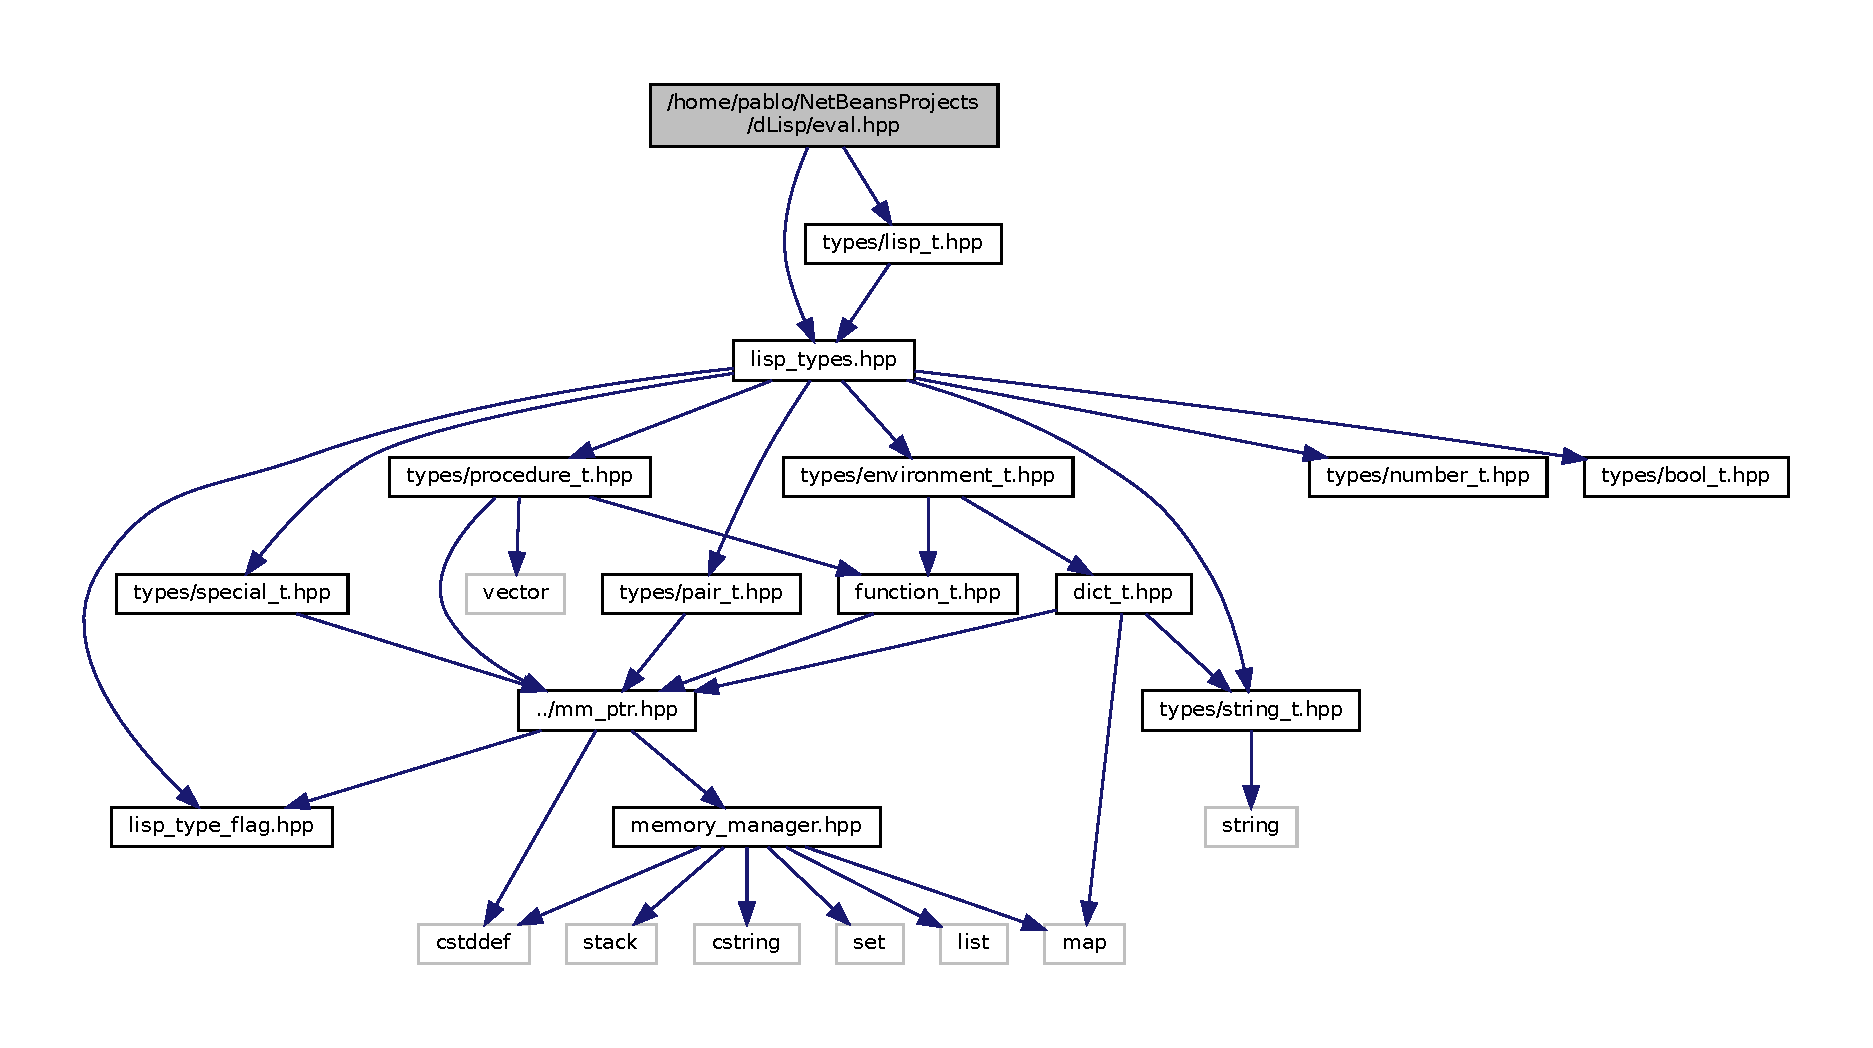
\includegraphics[width=350pt]{eval_8hpp__incl}
\end{center}
\end{figure}
\subsection*{Функции}
\begin{DoxyCompactItemize}
\item 
\mbox{\hyperlink{classmm__ptr}{obj\+\_\+ptr}} \mbox{\hyperlink{eval_8hpp_a4a0d1810add706542eab4500465e1b12}{eval}} (\mbox{\hyperlink{classmm__ptr}{obj\+\_\+ptr}}, \mbox{\hyperlink{classmm__ptr}{env\+\_\+ptr}})
\begin{DoxyCompactList}\small\item\em Вычисляет переданный ей список \end{DoxyCompactList}\item 
\mbox{\hyperlink{classmm__ptr}{obj\+\_\+ptr}} \mbox{\hyperlink{eval_8hpp_aedab4424101e323033774b107f805436}{evlis}} (\mbox{\hyperlink{classmm__ptr}{obj\+\_\+ptr}}, \mbox{\hyperlink{classmm__ptr}{env\+\_\+ptr}})
\begin{DoxyCompactList}\small\item\em Вычисляет каждый элемент списка и возвращает значение последнего \end{DoxyCompactList}\item 
\mbox{\hyperlink{classmm__ptr}{obj\+\_\+ptr}} \mbox{\hyperlink{eval_8hpp_af2d7bc77411eccbfc0fbab63edda7a7b}{eval\+\_\+exp}} (\mbox{\hyperlink{classmm__ptr}{obj\+\_\+ptr}}, \mbox{\hyperlink{classmm__ptr}{env\+\_\+ptr}})
\begin{DoxyCompactList}\small\item\em Вычисляет переданное ей выражение \end{DoxyCompactList}\end{DoxyCompactItemize}


\subsection{Подробное описание}
\begin{DoxyAuthor}{Автор}
\+: Павел Коваленко 
\end{DoxyAuthor}
\begin{DoxyDate}{Дата}
28 июля 2018 г., 16\+:05 
\end{DoxyDate}


\subsection{Функции}
\mbox{\Hypertarget{eval_8hpp_a4a0d1810add706542eab4500465e1b12}\label{eval_8hpp_a4a0d1810add706542eab4500465e1b12}} 
\index{eval.\+hpp@{eval.\+hpp}!eval@{eval}}
\index{eval@{eval}!eval.\+hpp@{eval.\+hpp}}
\subsubsection{\texorpdfstring{eval()}{eval()}}
{\footnotesize\ttfamily \mbox{\hyperlink{classmm__ptr}{obj\+\_\+ptr}} eval (\begin{DoxyParamCaption}\item[{\mbox{\hyperlink{classmm__ptr}{obj\+\_\+ptr}}}]{exp,  }\item[{\mbox{\hyperlink{classmm__ptr}{env\+\_\+ptr}}}]{env }\end{DoxyParamCaption})}



Вычисляет переданный ей список 


\begin{DoxyParams}{Аргументы}
{\em exp} & Список выражений на вычисление который возращает функция parse \\
\hline
{\em env} & Окружение в котором должно проходить вычисление \\
\hline
\end{DoxyParams}
\mbox{\Hypertarget{eval_8hpp_af2d7bc77411eccbfc0fbab63edda7a7b}\label{eval_8hpp_af2d7bc77411eccbfc0fbab63edda7a7b}} 
\index{eval.\+hpp@{eval.\+hpp}!eval\+\_\+exp@{eval\+\_\+exp}}
\index{eval\+\_\+exp@{eval\+\_\+exp}!eval.\+hpp@{eval.\+hpp}}
\subsubsection{\texorpdfstring{eval\+\_\+exp()}{eval\_exp()}}
{\footnotesize\ttfamily \mbox{\hyperlink{classmm__ptr}{obj\+\_\+ptr}} eval\+\_\+exp (\begin{DoxyParamCaption}\item[{\mbox{\hyperlink{classmm__ptr}{obj\+\_\+ptr}}}]{exp,  }\item[{\mbox{\hyperlink{classmm__ptr}{env\+\_\+ptr}}}]{env }\end{DoxyParamCaption})}



Вычисляет переданное ей выражение 


\begin{DoxyParams}{Аргументы}
{\em exp} & Выражение для вычисления \\
\hline
{\em env} & Окружение в котором должно проходить вычисление \\
\hline
\end{DoxyParams}
\mbox{\Hypertarget{eval_8hpp_aedab4424101e323033774b107f805436}\label{eval_8hpp_aedab4424101e323033774b107f805436}} 
\index{eval.\+hpp@{eval.\+hpp}!evlis@{evlis}}
\index{evlis@{evlis}!eval.\+hpp@{eval.\+hpp}}
\subsubsection{\texorpdfstring{evlis()}{evlis()}}
{\footnotesize\ttfamily \mbox{\hyperlink{classmm__ptr}{obj\+\_\+ptr}} evlis (\begin{DoxyParamCaption}\item[{\mbox{\hyperlink{classmm__ptr}{obj\+\_\+ptr}}}]{exp,  }\item[{\mbox{\hyperlink{classmm__ptr}{env\+\_\+ptr}}}]{env }\end{DoxyParamCaption})}



Вычисляет каждый элемент списка и возвращает значение последнего 


\begin{DoxyParams}{Аргументы}
{\em exp} & Список для вычисления  env Окружение в котором должно проходить вычисление \\
\hline
\end{DoxyParams}

\hypertarget{base_8hpp}{}\section{Файл /home/pablo/\+Net\+Beans\+Projects/d\+Lisp/lib/base.hpp}
\label{base_8hpp}\index{/home/pablo/\+Net\+Beans\+Projects/d\+Lisp/lib/base.\+hpp@{/home/pablo/\+Net\+Beans\+Projects/d\+Lisp/lib/base.\+hpp}}
{\ttfamily \#include \char`\"{}base/predicate.\+hpp\char`\"{}}\newline
{\ttfamily \#include \char`\"{}base/arithmetic.\+hpp\char`\"{}}\newline
Граф включаемых заголовочных файлов для base.\+hpp\+:
\nopagebreak
\begin{figure}[H]
\begin{center}
\leavevmode
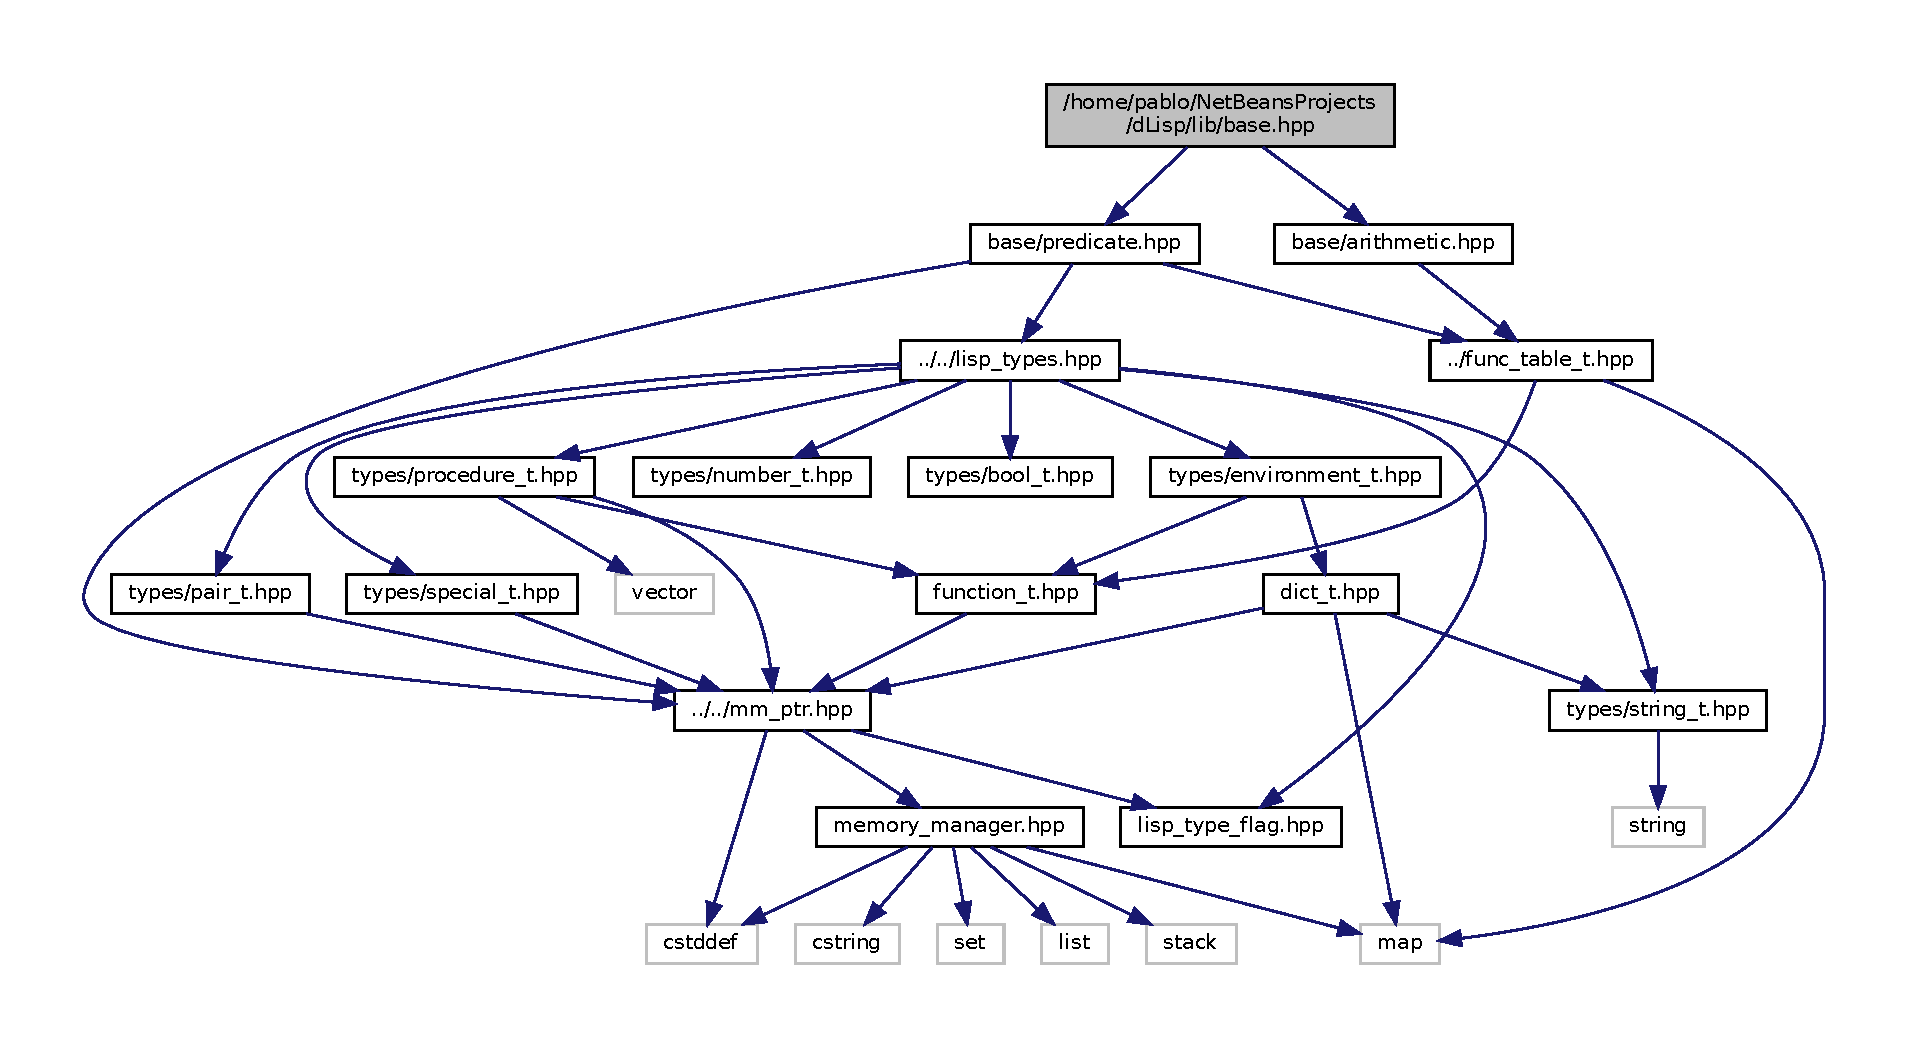
\includegraphics[width=350pt]{base_8hpp__incl}
\end{center}
\end{figure}


\subsection{Подробное описание}
\begin{DoxyAuthor}{Автор}
\+: Павел Коваленко 
\end{DoxyAuthor}
\begin{DoxyDate}{Дата}
13 августа 2018 г., 12\+:07
\end{DoxyDate}
Данный файл является основным для библиотеки base -\/ базовой библиотеки встроенной в интерпретатор. Base включает в себя
\begin{DoxyItemize}
\item predicate -\/ основные предикаты типов
\item arithmetic -\/ основные арифметические выражения 
\end{DoxyItemize}
\hypertarget{arithmetic_8hpp}{}\section{Файл /home/pablo/\+Net\+Beans\+Projects/d\+Lisp/lib/base/arithmetic.hpp}
\label{arithmetic_8hpp}\index{/home/pablo/\+Net\+Beans\+Projects/d\+Lisp/lib/base/arithmetic.\+hpp@{/home/pablo/\+Net\+Beans\+Projects/d\+Lisp/lib/base/arithmetic.\+hpp}}
{\ttfamily \#include \char`\"{}../func\+\_\+table\+\_\+t.\+hpp\char`\"{}}\newline
Граф включаемых заголовочных файлов для arithmetic.\+hpp\+:
\nopagebreak
\begin{figure}[H]
\begin{center}
\leavevmode
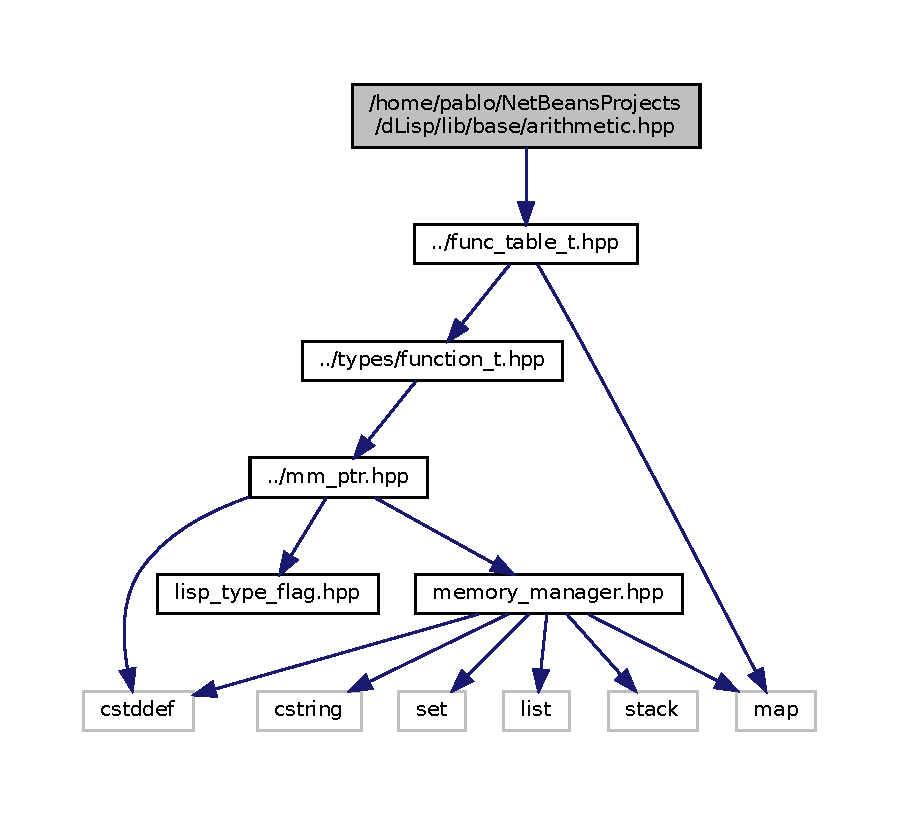
\includegraphics[width=350pt]{arithmetic_8hpp__incl}
\end{center}
\end{figure}
Граф файлов, в которые включается этот файл\+:
\nopagebreak
\begin{figure}[H]
\begin{center}
\leavevmode
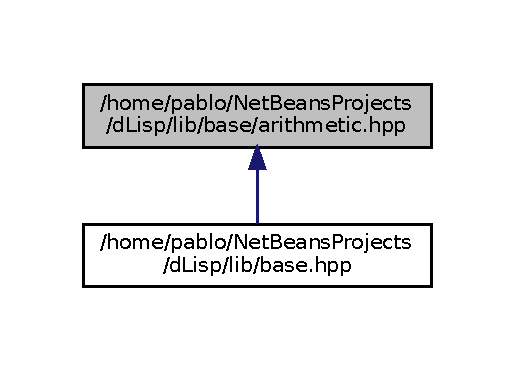
\includegraphics[width=247pt]{arithmetic_8hpp__dep__incl}
\end{center}
\end{figure}
\subsection*{Функции}
\begin{DoxyCompactItemize}
\item 
\mbox{\Hypertarget{arithmetic_8hpp_abbcbe9890dc718a5c1c0f50feba718f5}\label{arithmetic_8hpp_abbcbe9890dc718a5c1c0f50feba718f5}} 
\mbox{\hyperlink{classmm__ptr}{obj\+\_\+ptr}} \mbox{\hyperlink{arithmetic_8hpp_abbcbe9890dc718a5c1c0f50feba718f5}{add}} (\mbox{\hyperlink{classmm__ptr}{obj\+\_\+ptr}} obj, \mbox{\hyperlink{classmm__ptr}{env\+\_\+ptr}} env)
\begin{DoxyCompactList}\small\item\em Сложение \end{DoxyCompactList}\item 
\mbox{\Hypertarget{arithmetic_8hpp_a994439d99150718da8d18b4c027e9b3c}\label{arithmetic_8hpp_a994439d99150718da8d18b4c027e9b3c}} 
\mbox{\hyperlink{classmm__ptr}{obj\+\_\+ptr}} \mbox{\hyperlink{arithmetic_8hpp_a994439d99150718da8d18b4c027e9b3c}{sub}} (\mbox{\hyperlink{classmm__ptr}{obj\+\_\+ptr}} obj, \mbox{\hyperlink{classmm__ptr}{env\+\_\+ptr}} env)
\begin{DoxyCompactList}\small\item\em Вычитание \end{DoxyCompactList}\item 
\mbox{\Hypertarget{arithmetic_8hpp_a1a093be607b2da6051b98ee88f569d39}\label{arithmetic_8hpp_a1a093be607b2da6051b98ee88f569d39}} 
\mbox{\hyperlink{classmm__ptr}{obj\+\_\+ptr}} \mbox{\hyperlink{arithmetic_8hpp_a1a093be607b2da6051b98ee88f569d39}{multiply}} (\mbox{\hyperlink{classmm__ptr}{obj\+\_\+ptr}} obj, \mbox{\hyperlink{classmm__ptr}{env\+\_\+ptr}} env)
\begin{DoxyCompactList}\small\item\em Умножение \end{DoxyCompactList}\item 
\mbox{\Hypertarget{arithmetic_8hpp_add4c26d1ec3a1c005188e4c29299dcf0}\label{arithmetic_8hpp_add4c26d1ec3a1c005188e4c29299dcf0}} 
\mbox{\hyperlink{classmm__ptr}{obj\+\_\+ptr}} \mbox{\hyperlink{arithmetic_8hpp_add4c26d1ec3a1c005188e4c29299dcf0}{division}} (\mbox{\hyperlink{classmm__ptr}{obj\+\_\+ptr}} obj, \mbox{\hyperlink{classmm__ptr}{env\+\_\+ptr}} env)
\begin{DoxyCompactList}\small\item\em Деление \end{DoxyCompactList}\item 
\mbox{\Hypertarget{arithmetic_8hpp_a0b7d938a0b899f73f78cbf2ba924b7c8}\label{arithmetic_8hpp_a0b7d938a0b899f73f78cbf2ba924b7c8}} 
\mbox{\hyperlink{classmm__ptr}{obj\+\_\+ptr}} \mbox{\hyperlink{arithmetic_8hpp_a0b7d938a0b899f73f78cbf2ba924b7c8}{div}} (\mbox{\hyperlink{classmm__ptr}{obj\+\_\+ptr}} obj, \mbox{\hyperlink{classmm__ptr}{env\+\_\+ptr}} env)
\begin{DoxyCompactList}\small\item\em Целочисленное деление \end{DoxyCompactList}\item 
\mbox{\Hypertarget{arithmetic_8hpp_a448f1a760d94b90cb97021e034c4cb62}\label{arithmetic_8hpp_a448f1a760d94b90cb97021e034c4cb62}} 
\mbox{\hyperlink{classmm__ptr}{obj\+\_\+ptr}} \mbox{\hyperlink{arithmetic_8hpp_a448f1a760d94b90cb97021e034c4cb62}{mod}} (\mbox{\hyperlink{classmm__ptr}{obj\+\_\+ptr}} obj, \mbox{\hyperlink{classmm__ptr}{env\+\_\+ptr}} env)
\begin{DoxyCompactList}\small\item\em Остаток от деления \end{DoxyCompactList}\item 
\mbox{\Hypertarget{arithmetic_8hpp_ac059c79922330029d9fcf716622f7a49}\label{arithmetic_8hpp_ac059c79922330029d9fcf716622f7a49}} 
\mbox{\hyperlink{classmm__ptr}{obj\+\_\+ptr}} \mbox{\hyperlink{arithmetic_8hpp_ac059c79922330029d9fcf716622f7a49}{real\+\_\+p}} (\mbox{\hyperlink{classmm__ptr}{obj\+\_\+ptr}} obj, \mbox{\hyperlink{classmm__ptr}{env\+\_\+ptr}} env)
\begin{DoxyCompactList}\small\item\em Предикат проверяющий является ли число вещественным \end{DoxyCompactList}\item 
\mbox{\Hypertarget{arithmetic_8hpp_ae3710c07b832acce81b242efb06888d2}\label{arithmetic_8hpp_ae3710c07b832acce81b242efb06888d2}} 
\mbox{\hyperlink{classmm__ptr}{obj\+\_\+ptr}} \mbox{\hyperlink{arithmetic_8hpp_ae3710c07b832acce81b242efb06888d2}{int\+\_\+p}} (\mbox{\hyperlink{classmm__ptr}{obj\+\_\+ptr}} obj, \mbox{\hyperlink{classmm__ptr}{env\+\_\+ptr}} env)
\begin{DoxyCompactList}\small\item\em Предикат проверяющий является ли число целым \end{DoxyCompactList}\item 
\mbox{\Hypertarget{arithmetic_8hpp_aa012d022013772daf781dc16b3fe0eb0}\label{arithmetic_8hpp_aa012d022013772daf781dc16b3fe0eb0}} 
\mbox{\hyperlink{classmm__ptr}{obj\+\_\+ptr}} \mbox{\hyperlink{arithmetic_8hpp_aa012d022013772daf781dc16b3fe0eb0}{eq\+\_\+np}} (\mbox{\hyperlink{classmm__ptr}{obj\+\_\+ptr}} obj, \mbox{\hyperlink{classmm__ptr}{env\+\_\+ptr}} env)
\begin{DoxyCompactList}\small\item\em Равенство чисел \end{DoxyCompactList}\item 
\mbox{\Hypertarget{arithmetic_8hpp_ad1a6045662ea9ed831ca9c828a217215}\label{arithmetic_8hpp_ad1a6045662ea9ed831ca9c828a217215}} 
\mbox{\hyperlink{classmm__ptr}{obj\+\_\+ptr}} \mbox{\hyperlink{arithmetic_8hpp_ad1a6045662ea9ed831ca9c828a217215}{less\+\_\+np}} (\mbox{\hyperlink{classmm__ptr}{obj\+\_\+ptr}} obj, \mbox{\hyperlink{classmm__ptr}{env\+\_\+ptr}} env)
\begin{DoxyCompactList}\small\item\em Меньше \end{DoxyCompactList}\item 
\mbox{\Hypertarget{arithmetic_8hpp_a907719e1715d083332c4c6894ba22f5e}\label{arithmetic_8hpp_a907719e1715d083332c4c6894ba22f5e}} 
\mbox{\hyperlink{classmm__ptr}{obj\+\_\+ptr}} \mbox{\hyperlink{arithmetic_8hpp_a907719e1715d083332c4c6894ba22f5e}{greater\+\_\+np}} (\mbox{\hyperlink{classmm__ptr}{obj\+\_\+ptr}} obj, \mbox{\hyperlink{classmm__ptr}{env\+\_\+ptr}} env)
\begin{DoxyCompactList}\small\item\em Больше \end{DoxyCompactList}\item 
\mbox{\Hypertarget{arithmetic_8hpp_afdbdfce5b566c542256143c34a98f9cf}\label{arithmetic_8hpp_afdbdfce5b566c542256143c34a98f9cf}} 
\mbox{\hyperlink{classmm__ptr}{obj\+\_\+ptr}} \mbox{\hyperlink{arithmetic_8hpp_afdbdfce5b566c542256143c34a98f9cf}{lte\+\_\+np}} (\mbox{\hyperlink{classmm__ptr}{obj\+\_\+ptr}} obj, \mbox{\hyperlink{classmm__ptr}{env\+\_\+ptr}} env)
\begin{DoxyCompactList}\small\item\em Меньше либо равно \end{DoxyCompactList}\item 
\mbox{\Hypertarget{arithmetic_8hpp_a2fe6e322325b3be4d88a9fadf3bf8467}\label{arithmetic_8hpp_a2fe6e322325b3be4d88a9fadf3bf8467}} 
\mbox{\hyperlink{classmm__ptr}{obj\+\_\+ptr}} \mbox{\hyperlink{arithmetic_8hpp_a2fe6e322325b3be4d88a9fadf3bf8467}{gte\+\_\+np}} (\mbox{\hyperlink{classmm__ptr}{obj\+\_\+ptr}} obj, \mbox{\hyperlink{classmm__ptr}{env\+\_\+ptr}} env)
\begin{DoxyCompactList}\small\item\em Больше либо равно \end{DoxyCompactList}\end{DoxyCompactItemize}
\subsection*{Переменные}
\begin{DoxyCompactItemize}
\item 
const \mbox{\hyperlink{func__table__t_8hpp_af845869dd1e42c662a4b4f00d1fc528d}{func\+\_\+table\+\_\+t}} {\bfseries base\+\_\+arithmetic\+::func\+\_\+table}
\end{DoxyCompactItemize}


\subsection{Подробное описание}
\begin{DoxyAuthor}{Автор}
\+: Павел Коваленко 
\end{DoxyAuthor}
\begin{DoxyDate}{Дата}
14 августа 2018 г., 12\+:44
\end{DoxyDate}
Данный файл содержит определения арифметических процедур предоставляемых библиотекой base 

\subsection{Переменные}
\mbox{\Hypertarget{arithmetic_8hpp_file_a3b46aafb8a45dd810dcf047013742190}\label{arithmetic_8hpp_file_a3b46aafb8a45dd810dcf047013742190}} 
\index{arithmetic.\+hpp@{arithmetic.\+hpp}!func\+\_\+table@{func\+\_\+table}}
\index{func\+\_\+table@{func\+\_\+table}!arithmetic.\+hpp@{arithmetic.\+hpp}}
\subsubsection{\texorpdfstring{func\+\_\+table}{func\_table}}
{\footnotesize\ttfamily const \mbox{\hyperlink{func__table__t_8hpp_af845869dd1e42c662a4b4f00d1fc528d}{func\+\_\+table\+\_\+t}} base\+\_\+arithmetic\+::func\+\_\+table}

{\bfseries Инициализатор}
\begin{DoxyCode}
= \{
        \{\textcolor{stringliteral}{"+"}, \mbox{\hyperlink{func__table__t_8hpp_a2997b2f150bf75a930fa2943a5fc6a35}{p}}(\mbox{\hyperlink{arithmetic_8hpp_abbcbe9890dc718a5c1c0f50feba718f5}{add}}, 2)\},
        \{\textcolor{stringliteral}{"-"}, \mbox{\hyperlink{func__table__t_8hpp_a2997b2f150bf75a930fa2943a5fc6a35}{p}}(\mbox{\hyperlink{arithmetic_8hpp_a994439d99150718da8d18b4c027e9b3c}{sub}}, 2)\},
        \{\textcolor{stringliteral}{"*"}, \mbox{\hyperlink{func__table__t_8hpp_a2997b2f150bf75a930fa2943a5fc6a35}{p}}(\mbox{\hyperlink{arithmetic_8hpp_a1a093be607b2da6051b98ee88f569d39}{multiply}}, 2)\},
        \{\textcolor{stringliteral}{"/"}, \mbox{\hyperlink{func__table__t_8hpp_a2997b2f150bf75a930fa2943a5fc6a35}{p}}(\mbox{\hyperlink{arithmetic_8hpp_add4c26d1ec3a1c005188e4c29299dcf0}{division}}, 2)\},
        \{\textcolor{stringliteral}{"div"}, \mbox{\hyperlink{func__table__t_8hpp_a2997b2f150bf75a930fa2943a5fc6a35}{p}}(\mbox{\hyperlink{arithmetic_8hpp_a0b7d938a0b899f73f78cbf2ba924b7c8}{div}}, 2)\},
        \{\textcolor{stringliteral}{"mod"}, \mbox{\hyperlink{func__table__t_8hpp_a2997b2f150bf75a930fa2943a5fc6a35}{p}}(\mbox{\hyperlink{arithmetic_8hpp_a448f1a760d94b90cb97021e034c4cb62}{mod}}, 2)\},
        \{\textcolor{stringliteral}{"real?"}, \mbox{\hyperlink{func__table__t_8hpp_a2997b2f150bf75a930fa2943a5fc6a35}{p}}(\mbox{\hyperlink{arithmetic_8hpp_ac059c79922330029d9fcf716622f7a49}{real\_p}}, 1)\},
        \{\textcolor{stringliteral}{"integer?"}, \mbox{\hyperlink{func__table__t_8hpp_a2997b2f150bf75a930fa2943a5fc6a35}{p}}(\mbox{\hyperlink{arithmetic_8hpp_ae3710c07b832acce81b242efb06888d2}{int\_p}}, 1)\},
        \{\textcolor{stringliteral}{"="}, \mbox{\hyperlink{func__table__t_8hpp_a2997b2f150bf75a930fa2943a5fc6a35}{p}}(\mbox{\hyperlink{arithmetic_8hpp_aa012d022013772daf781dc16b3fe0eb0}{eq\_np}}, 2)\},
        \{\textcolor{stringliteral}{"<"}, \mbox{\hyperlink{func__table__t_8hpp_a2997b2f150bf75a930fa2943a5fc6a35}{p}}(\mbox{\hyperlink{arithmetic_8hpp_ad1a6045662ea9ed831ca9c828a217215}{less\_np}}, 2)\},
        \{\textcolor{stringliteral}{">"}, \mbox{\hyperlink{func__table__t_8hpp_a2997b2f150bf75a930fa2943a5fc6a35}{p}}(\mbox{\hyperlink{arithmetic_8hpp_a907719e1715d083332c4c6894ba22f5e}{greater\_np}}, 2)\},
        \{\textcolor{stringliteral}{"<="}, \mbox{\hyperlink{func__table__t_8hpp_a2997b2f150bf75a930fa2943a5fc6a35}{p}}(\mbox{\hyperlink{arithmetic_8hpp_afdbdfce5b566c542256143c34a98f9cf}{lte\_np}}, 2)\},
        \{\textcolor{stringliteral}{">="}, \mbox{\hyperlink{func__table__t_8hpp_a2997b2f150bf75a930fa2943a5fc6a35}{p}}(\mbox{\hyperlink{arithmetic_8hpp_a2fe6e322325b3be4d88a9fadf3bf8467}{gte\_np}}, 2)\}
    \}
\end{DoxyCode}

\hypertarget{func__table__t_8hpp}{}\section{Файл /home/pablo/\+Net\+Beans\+Projects/d\+Lisp/lib/func\+\_\+table\+\_\+t.hpp}
\label{func__table__t_8hpp}\index{/home/pablo/\+Net\+Beans\+Projects/d\+Lisp/lib/func\+\_\+table\+\_\+t.\+hpp@{/home/pablo/\+Net\+Beans\+Projects/d\+Lisp/lib/func\+\_\+table\+\_\+t.\+hpp}}
{\ttfamily \#include \char`\"{}../types/function\+\_\+t.\+hpp\char`\"{}}\newline
{\ttfamily \#include $<$map$>$}\newline
Граф включаемых заголовочных файлов для func\+\_\+table\+\_\+t.\+hpp\+:
\nopagebreak
\begin{figure}[H]
\begin{center}
\leavevmode
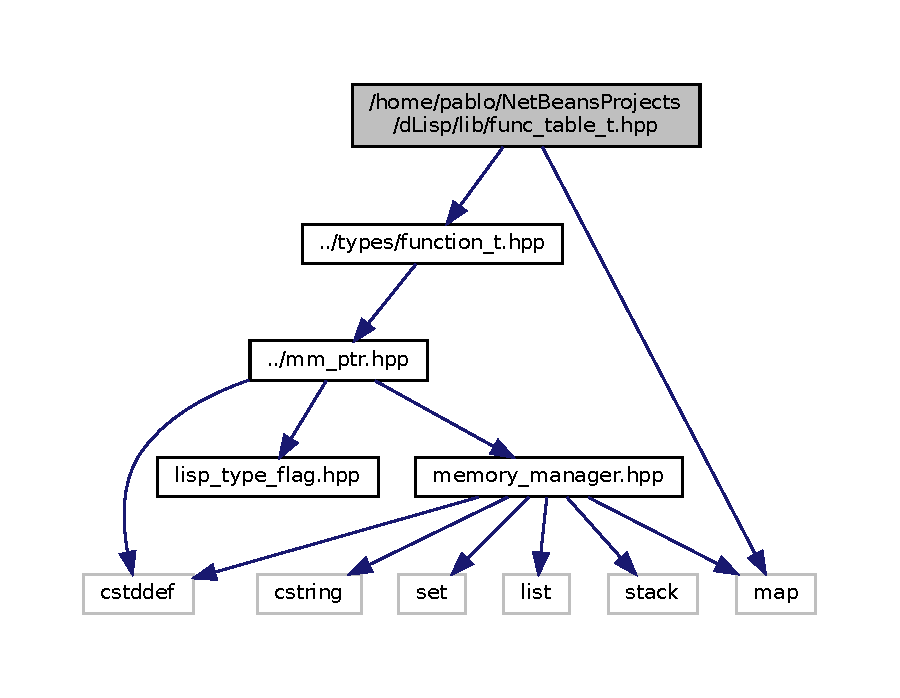
\includegraphics[width=350pt]{func__table__t_8hpp__incl}
\end{center}
\end{figure}
Граф файлов, в которые включается этот файл\+:
\nopagebreak
\begin{figure}[H]
\begin{center}
\leavevmode
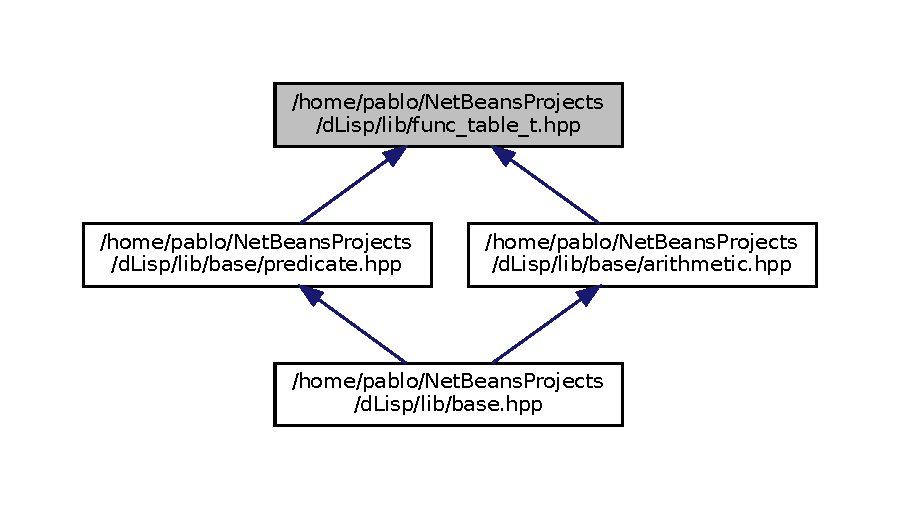
\includegraphics[width=350pt]{func__table__t_8hpp__dep__incl}
\end{center}
\end{figure}
\subsection*{Макросы}
\begin{DoxyCompactItemize}
\item 
\mbox{\Hypertarget{func__table__t_8hpp_a2997b2f150bf75a930fa2943a5fc6a35}\label{func__table__t_8hpp_a2997b2f150bf75a930fa2943a5fc6a35}} 
\#define \mbox{\hyperlink{func__table__t_8hpp_a2997b2f150bf75a930fa2943a5fc6a35}{p}}(f,  n)~std\+::make\+\_\+pair$<$function\+\_\+t, size\+\_\+t$>$(f, n)
\begin{DoxyCompactList}\small\item\em Создание пары (функция, кол-\/во параметров) \end{DoxyCompactList}\item 
\mbox{\Hypertarget{func__table__t_8hpp_a24a19fb822a3badedc1c6bd27883c8ef}\label{func__table__t_8hpp_a24a19fb822a3badedc1c6bd27883c8ef}} 
\#define \mbox{\hyperlink{func__table__t_8hpp_a24a19fb822a3badedc1c6bd27883c8ef}{make\+\_\+number}}(n)~make\+\_\+object(\mbox{\hyperlink{lisp__type__flag_8hpp_a055b7e4c72b7a614806ae1225539b99fa9d873df6e994539eb7566bd3a1ebaef3}{T\+\_\+\+N\+U\+M\+B\+ER}}, \mbox{\hyperlink{classnumber__t}{number\+\_\+t}}((n)))
\begin{DoxyCompactList}\small\item\em Создание числа \end{DoxyCompactList}\item 
\mbox{\Hypertarget{func__table__t_8hpp_aea3a3ece078763f094bada731a6d862f}\label{func__table__t_8hpp_aea3a3ece078763f094bada731a6d862f}} 
\#define \mbox{\hyperlink{func__table__t_8hpp_aea3a3ece078763f094bada731a6d862f}{make\+\_\+bool}}(\mbox{\hyperlink{func__table__t_8hpp_a2997b2f150bf75a930fa2943a5fc6a35}{p}})~make\+\_\+object(\mbox{\hyperlink{lisp__type__flag_8hpp_a055b7e4c72b7a614806ae1225539b99fa7af48b89eafa6f3fc499363a6189f2cf}{T\+\_\+\+B\+O\+OL}}, \mbox{\hyperlink{classbool__t}{bool\+\_\+t}}((\mbox{\hyperlink{func__table__t_8hpp_a2997b2f150bf75a930fa2943a5fc6a35}{p}})))
\begin{DoxyCompactList}\small\item\em Создание булевого значения \end{DoxyCompactList}\end{DoxyCompactItemize}
\subsection*{Определения типов}
\begin{DoxyCompactItemize}
\item 
\mbox{\Hypertarget{func__table__t_8hpp_af845869dd1e42c662a4b4f00d1fc528d}\label{func__table__t_8hpp_af845869dd1e42c662a4b4f00d1fc528d}} 
using \mbox{\hyperlink{func__table__t_8hpp_af845869dd1e42c662a4b4f00d1fc528d}{func\+\_\+table\+\_\+t}} = std\+::map$<$ const char $\ast$, std\+::pair$<$ function\+\_\+t, size\+\_\+t $>$ $>$
\begin{DoxyCompactList}\small\item\em Определяет таблицу функций используемую как интерфейс для библиотек \end{DoxyCompactList}\end{DoxyCompactItemize}


\subsection{Подробное описание}
\begin{DoxyAuthor}{Автор}
\+: Павел Коваленко 
\end{DoxyAuthor}
\begin{DoxyDate}{Дата}
13 августа 2018 г., 12\+:49 
\end{DoxyDate}

\hypertarget{lisp__type__flag_8hpp}{}\section{Файл /home/pablo/\+Net\+Beans\+Projects/d\+Lisp/lisp\+\_\+type\+\_\+flag.hpp}
\label{lisp__type__flag_8hpp}\index{/home/pablo/\+Net\+Beans\+Projects/d\+Lisp/lisp\+\_\+type\+\_\+flag.\+hpp@{/home/pablo/\+Net\+Beans\+Projects/d\+Lisp/lisp\+\_\+type\+\_\+flag.\+hpp}}
Граф файлов, в которые включается этот файл\+:
\nopagebreak
\begin{figure}[H]
\begin{center}
\leavevmode
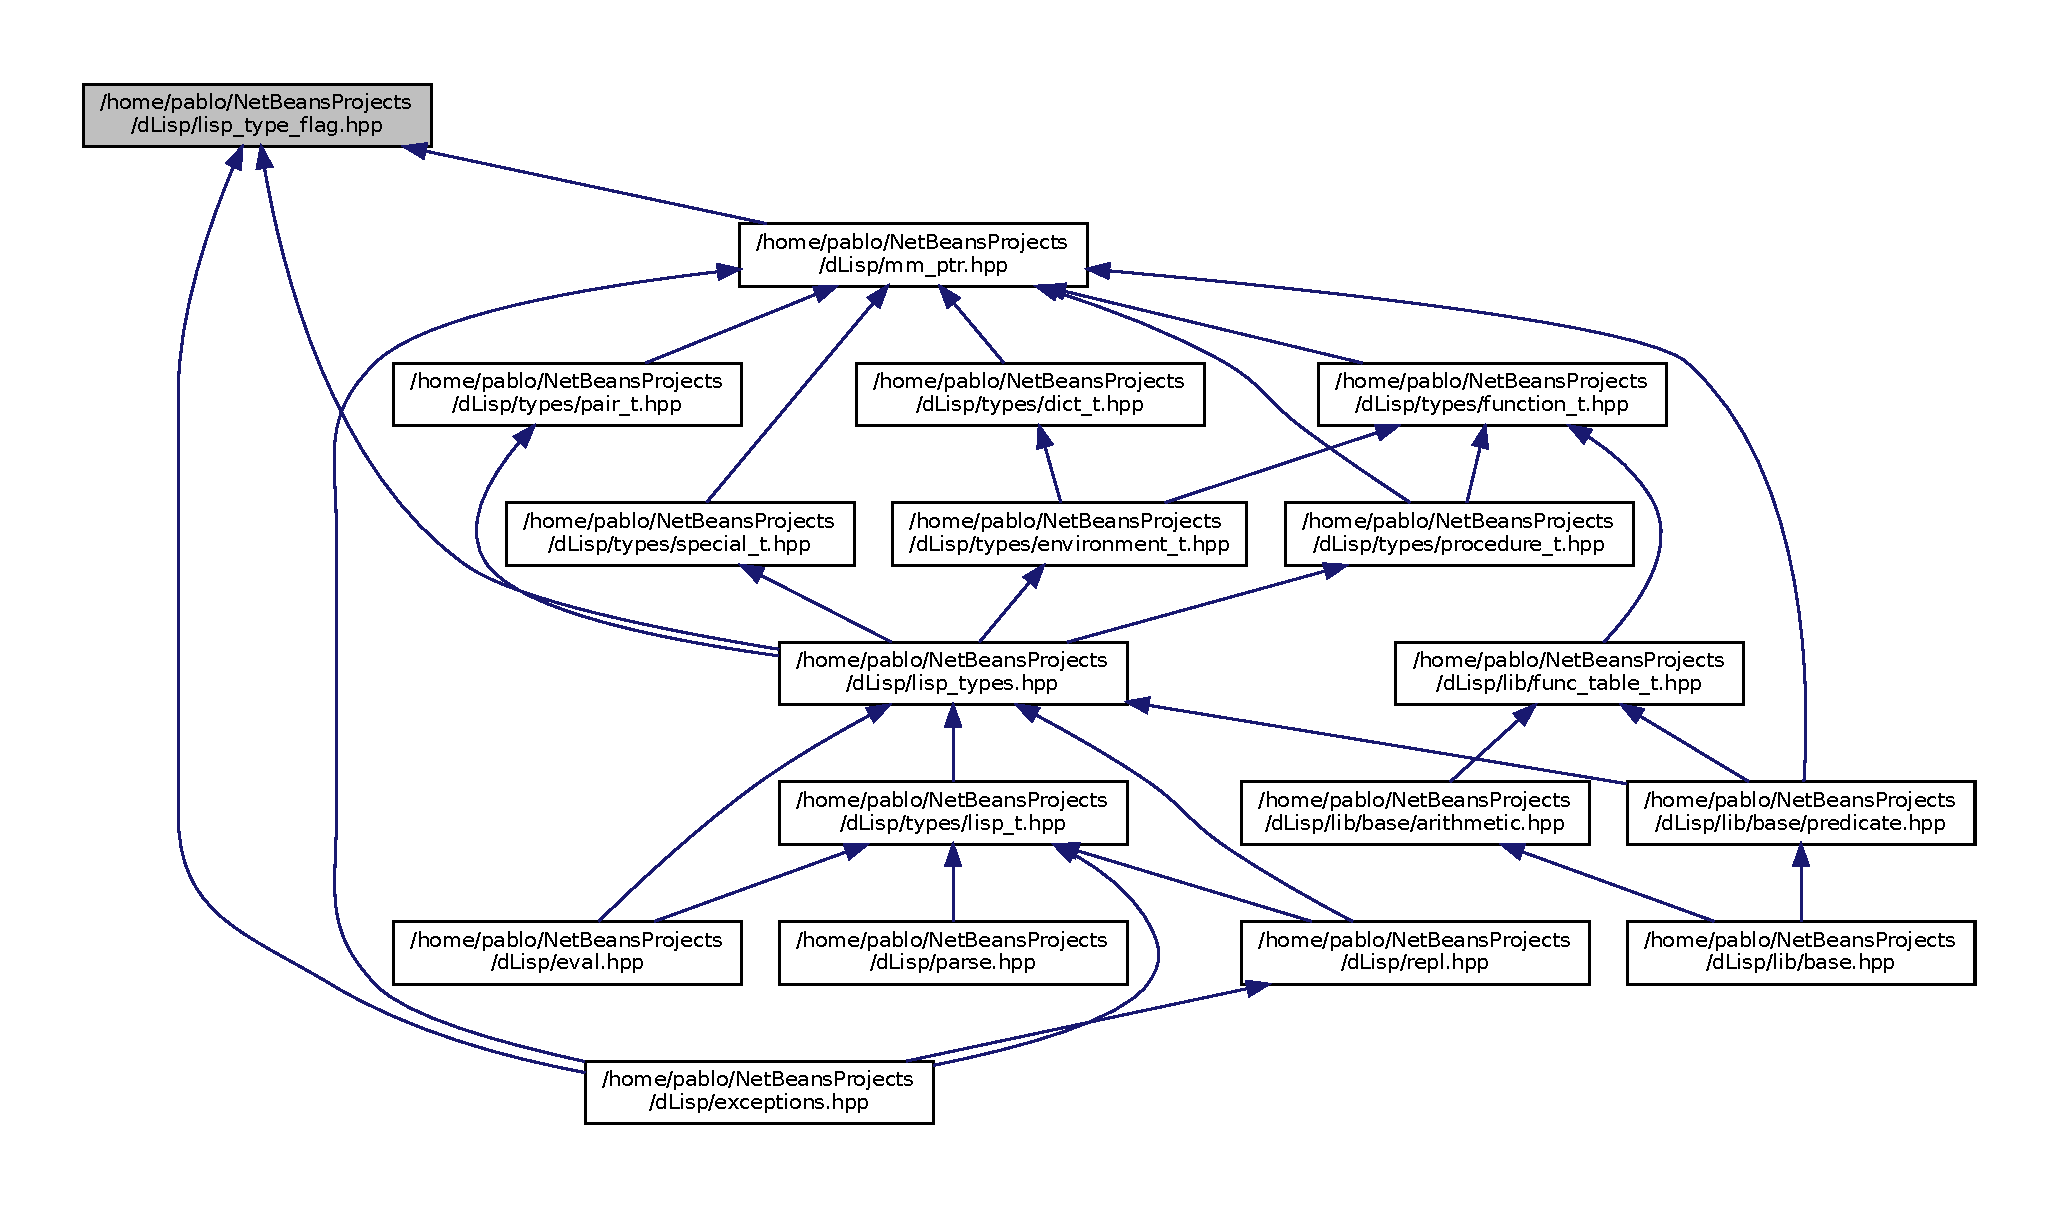
\includegraphics[width=350pt]{lisp__type__flag_8hpp__dep__incl}
\end{center}
\end{figure}
\subsection*{Перечисления}
\begin{DoxyCompactItemize}
\item 
enum \mbox{\hyperlink{lisp__type__flag_8hpp_a055b7e4c72b7a614806ae1225539b99f}{lisp\+\_\+type\+\_\+flag}} \+: char \{ \newline
\mbox{\hyperlink{lisp__type__flag_8hpp_a055b7e4c72b7a614806ae1225539b99fa26c5769a44ea25ffe1407c6a0bfdb862}{T\+\_\+\+N\+U\+LL}}, 
\mbox{\hyperlink{lisp__type__flag_8hpp_a055b7e4c72b7a614806ae1225539b99fa58711dadadce623c4e93f806c71ea4d7}{T\+\_\+\+S\+P\+E\+C\+I\+AL}}, 
\mbox{\hyperlink{lisp__type__flag_8hpp_a055b7e4c72b7a614806ae1225539b99fa7af48b89eafa6f3fc499363a6189f2cf}{T\+\_\+\+B\+O\+OL}}, 
\mbox{\hyperlink{lisp__type__flag_8hpp_a055b7e4c72b7a614806ae1225539b99fa9d873df6e994539eb7566bd3a1ebaef3}{T\+\_\+\+N\+U\+M\+B\+ER}}, 
\newline
\mbox{\hyperlink{lisp__type__flag_8hpp_a055b7e4c72b7a614806ae1225539b99fa2b93aac4bda1ecc9cd242c671411c323}{T\+\_\+\+S\+T\+R\+I\+NG}}, 
\mbox{\hyperlink{lisp__type__flag_8hpp_a055b7e4c72b7a614806ae1225539b99faf1e8ae4f66ff018bac0f672bd588178c}{T\+\_\+\+S\+Y\+M\+B\+OL}}, 
\mbox{\hyperlink{lisp__type__flag_8hpp_a055b7e4c72b7a614806ae1225539b99fa2d8a18ddbcfddef75235dcebed5de2b2}{T\+\_\+\+P\+A\+IR}}, 
\mbox{\hyperlink{lisp__type__flag_8hpp_a055b7e4c72b7a614806ae1225539b99fa0d3277a2ebb08338d2f4887f77a1cb7a}{T\+\_\+\+P\+R\+OC}}, 
\newline
\mbox{\hyperlink{lisp__type__flag_8hpp_a055b7e4c72b7a614806ae1225539b99fa7dbf71528f3c7622568c3bbdcb6c1724}{T\+\_\+\+E\+NV}}
 \}
\begin{DoxyCompactList}\small\item\em Флаги типов lisp-\/объектов \end{DoxyCompactList}\end{DoxyCompactItemize}


\subsection{Подробное описание}
\begin{DoxyAuthor}{Автор}
\+: Павел Коваленко 
\end{DoxyAuthor}
\begin{DoxyDate}{Дата}
2 августа 2018 г., 2\+:32 
\end{DoxyDate}


\subsection{Перечисления}
\mbox{\Hypertarget{lisp__type__flag_8hpp_a055b7e4c72b7a614806ae1225539b99f}\label{lisp__type__flag_8hpp_a055b7e4c72b7a614806ae1225539b99f}} 
\index{lisp\+\_\+type\+\_\+flag.\+hpp@{lisp\+\_\+type\+\_\+flag.\+hpp}!lisp\+\_\+type\+\_\+flag@{lisp\+\_\+type\+\_\+flag}}
\index{lisp\+\_\+type\+\_\+flag@{lisp\+\_\+type\+\_\+flag}!lisp\+\_\+type\+\_\+flag.\+hpp@{lisp\+\_\+type\+\_\+flag.\+hpp}}
\subsubsection{\texorpdfstring{lisp\+\_\+type\+\_\+flag}{lisp\_type\_flag}}
{\footnotesize\ttfamily enum \mbox{\hyperlink{lisp__type__flag_8hpp_a055b7e4c72b7a614806ae1225539b99f}{lisp\+\_\+type\+\_\+flag}} \+: char}



Флаги типов lisp-\/объектов 

\begin{DoxyEnumFields}{Элементы перечислений}
\raisebox{\heightof{T}}[0pt][0pt]{\index{T\+\_\+\+N\+U\+LL@{T\+\_\+\+N\+U\+LL}!lisp\+\_\+type\+\_\+flag.\+hpp@{lisp\+\_\+type\+\_\+flag.\+hpp}}\index{lisp\+\_\+type\+\_\+flag.\+hpp@{lisp\+\_\+type\+\_\+flag.\+hpp}!T\+\_\+\+N\+U\+LL@{T\+\_\+\+N\+U\+LL}}}\mbox{\Hypertarget{lisp__type__flag_8hpp_a055b7e4c72b7a614806ae1225539b99fa26c5769a44ea25ffe1407c6a0bfdb862}\label{lisp__type__flag_8hpp_a055b7e4c72b7a614806ae1225539b99fa26c5769a44ea25ffe1407c6a0bfdb862}} 
T\+\_\+\+N\+U\+LL&Флаг типа пустого списка () \\
\hline

\raisebox{\heightof{T}}[0pt][0pt]{\index{T\+\_\+\+S\+P\+E\+C\+I\+AL@{T\+\_\+\+S\+P\+E\+C\+I\+AL}!lisp\+\_\+type\+\_\+flag.\+hpp@{lisp\+\_\+type\+\_\+flag.\+hpp}}\index{lisp\+\_\+type\+\_\+flag.\+hpp@{lisp\+\_\+type\+\_\+flag.\+hpp}!T\+\_\+\+S\+P\+E\+C\+I\+AL@{T\+\_\+\+S\+P\+E\+C\+I\+AL}}}\mbox{\Hypertarget{lisp__type__flag_8hpp_a055b7e4c72b7a614806ae1225539b99fa58711dadadce623c4e93f806c71ea4d7}\label{lisp__type__flag_8hpp_a055b7e4c72b7a614806ae1225539b99fa58711dadadce623c4e93f806c71ea4d7}} 
T\+\_\+\+S\+P\+E\+C\+I\+AL&Флаг специального типа \\
\hline

\raisebox{\heightof{T}}[0pt][0pt]{\index{T\+\_\+\+B\+O\+OL@{T\+\_\+\+B\+O\+OL}!lisp\+\_\+type\+\_\+flag.\+hpp@{lisp\+\_\+type\+\_\+flag.\+hpp}}\index{lisp\+\_\+type\+\_\+flag.\+hpp@{lisp\+\_\+type\+\_\+flag.\+hpp}!T\+\_\+\+B\+O\+OL@{T\+\_\+\+B\+O\+OL}}}\mbox{\Hypertarget{lisp__type__flag_8hpp_a055b7e4c72b7a614806ae1225539b99fa7af48b89eafa6f3fc499363a6189f2cf}\label{lisp__type__flag_8hpp_a055b7e4c72b7a614806ae1225539b99fa7af48b89eafa6f3fc499363a6189f2cf}} 
T\+\_\+\+B\+O\+OL&Флаг логического (булевого) типа \\
\hline

\raisebox{\heightof{T}}[0pt][0pt]{\index{T\+\_\+\+N\+U\+M\+B\+ER@{T\+\_\+\+N\+U\+M\+B\+ER}!lisp\+\_\+type\+\_\+flag.\+hpp@{lisp\+\_\+type\+\_\+flag.\+hpp}}\index{lisp\+\_\+type\+\_\+flag.\+hpp@{lisp\+\_\+type\+\_\+flag.\+hpp}!T\+\_\+\+N\+U\+M\+B\+ER@{T\+\_\+\+N\+U\+M\+B\+ER}}}\mbox{\Hypertarget{lisp__type__flag_8hpp_a055b7e4c72b7a614806ae1225539b99fa9d873df6e994539eb7566bd3a1ebaef3}\label{lisp__type__flag_8hpp_a055b7e4c72b7a614806ae1225539b99fa9d873df6e994539eb7566bd3a1ebaef3}} 
T\+\_\+\+N\+U\+M\+B\+ER&Флаг числового типа \\
\hline

\raisebox{\heightof{T}}[0pt][0pt]{\index{T\+\_\+\+S\+T\+R\+I\+NG@{T\+\_\+\+S\+T\+R\+I\+NG}!lisp\+\_\+type\+\_\+flag.\+hpp@{lisp\+\_\+type\+\_\+flag.\+hpp}}\index{lisp\+\_\+type\+\_\+flag.\+hpp@{lisp\+\_\+type\+\_\+flag.\+hpp}!T\+\_\+\+S\+T\+R\+I\+NG@{T\+\_\+\+S\+T\+R\+I\+NG}}}\mbox{\Hypertarget{lisp__type__flag_8hpp_a055b7e4c72b7a614806ae1225539b99fa2b93aac4bda1ecc9cd242c671411c323}\label{lisp__type__flag_8hpp_a055b7e4c72b7a614806ae1225539b99fa2b93aac4bda1ecc9cd242c671411c323}} 
T\+\_\+\+S\+T\+R\+I\+NG&Флаг типа строки \\
\hline

\raisebox{\heightof{T}}[0pt][0pt]{\index{T\+\_\+\+S\+Y\+M\+B\+OL@{T\+\_\+\+S\+Y\+M\+B\+OL}!lisp\+\_\+type\+\_\+flag.\+hpp@{lisp\+\_\+type\+\_\+flag.\+hpp}}\index{lisp\+\_\+type\+\_\+flag.\+hpp@{lisp\+\_\+type\+\_\+flag.\+hpp}!T\+\_\+\+S\+Y\+M\+B\+OL@{T\+\_\+\+S\+Y\+M\+B\+OL}}}\mbox{\Hypertarget{lisp__type__flag_8hpp_a055b7e4c72b7a614806ae1225539b99faf1e8ae4f66ff018bac0f672bd588178c}\label{lisp__type__flag_8hpp_a055b7e4c72b7a614806ae1225539b99faf1e8ae4f66ff018bac0f672bd588178c}} 
T\+\_\+\+S\+Y\+M\+B\+OL&Флаг типа символа \\
\hline

\raisebox{\heightof{T}}[0pt][0pt]{\index{T\+\_\+\+P\+A\+IR@{T\+\_\+\+P\+A\+IR}!lisp\+\_\+type\+\_\+flag.\+hpp@{lisp\+\_\+type\+\_\+flag.\+hpp}}\index{lisp\+\_\+type\+\_\+flag.\+hpp@{lisp\+\_\+type\+\_\+flag.\+hpp}!T\+\_\+\+P\+A\+IR@{T\+\_\+\+P\+A\+IR}}}\mbox{\Hypertarget{lisp__type__flag_8hpp_a055b7e4c72b7a614806ae1225539b99fa2d8a18ddbcfddef75235dcebed5de2b2}\label{lisp__type__flag_8hpp_a055b7e4c72b7a614806ae1225539b99fa2d8a18ddbcfddef75235dcebed5de2b2}} 
T\+\_\+\+P\+A\+IR&Флаг типа пары \\
\hline

\raisebox{\heightof{T}}[0pt][0pt]{\index{T\+\_\+\+P\+R\+OC@{T\+\_\+\+P\+R\+OC}!lisp\+\_\+type\+\_\+flag.\+hpp@{lisp\+\_\+type\+\_\+flag.\+hpp}}\index{lisp\+\_\+type\+\_\+flag.\+hpp@{lisp\+\_\+type\+\_\+flag.\+hpp}!T\+\_\+\+P\+R\+OC@{T\+\_\+\+P\+R\+OC}}}\mbox{\Hypertarget{lisp__type__flag_8hpp_a055b7e4c72b7a614806ae1225539b99fa0d3277a2ebb08338d2f4887f77a1cb7a}\label{lisp__type__flag_8hpp_a055b7e4c72b7a614806ae1225539b99fa0d3277a2ebb08338d2f4887f77a1cb7a}} 
T\+\_\+\+P\+R\+OC&Флаг типа процедуры \\
\hline

\raisebox{\heightof{T}}[0pt][0pt]{\index{T\+\_\+\+E\+NV@{T\+\_\+\+E\+NV}!lisp\+\_\+type\+\_\+flag.\+hpp@{lisp\+\_\+type\+\_\+flag.\+hpp}}\index{lisp\+\_\+type\+\_\+flag.\+hpp@{lisp\+\_\+type\+\_\+flag.\+hpp}!T\+\_\+\+E\+NV@{T\+\_\+\+E\+NV}}}\mbox{\Hypertarget{lisp__type__flag_8hpp_a055b7e4c72b7a614806ae1225539b99fa7dbf71528f3c7622568c3bbdcb6c1724}\label{lisp__type__flag_8hpp_a055b7e4c72b7a614806ae1225539b99fa7dbf71528f3c7622568c3bbdcb6c1724}} 
T\+\_\+\+E\+NV&Флаг типа окружения \\
\hline

\end{DoxyEnumFields}

\hypertarget{lisp__types_8hpp}{}\section{Файл /home/pablo/\+Net\+Beans\+Projects/d\+Lisp/lisp\+\_\+types.hpp}
\label{lisp__types_8hpp}\index{/home/pablo/\+Net\+Beans\+Projects/d\+Lisp/lisp\+\_\+types.\+hpp@{/home/pablo/\+Net\+Beans\+Projects/d\+Lisp/lisp\+\_\+types.\+hpp}}
{\ttfamily \#include \char`\"{}lisp\+\_\+type\+\_\+flag.\+hpp\char`\"{}}\newline
{\ttfamily \#include \char`\"{}types/number\+\_\+t.\+hpp\char`\"{}}\newline
{\ttfamily \#include \char`\"{}types/string\+\_\+t.\+hpp\char`\"{}}\newline
{\ttfamily \#include \char`\"{}types/bool\+\_\+t.\+hpp\char`\"{}}\newline
{\ttfamily \#include \char`\"{}types/special\+\_\+t.\+hpp\char`\"{}}\newline
{\ttfamily \#include \char`\"{}types/procedure\+\_\+t.\+hpp\char`\"{}}\newline
{\ttfamily \#include \char`\"{}types/pair\+\_\+t.\+hpp\char`\"{}}\newline
{\ttfamily \#include \char`\"{}types/environment\+\_\+t.\+hpp\char`\"{}}\newline
Граф включаемых заголовочных файлов для lisp\+\_\+types.\+hpp\+:
\nopagebreak
\begin{figure}[H]
\begin{center}
\leavevmode
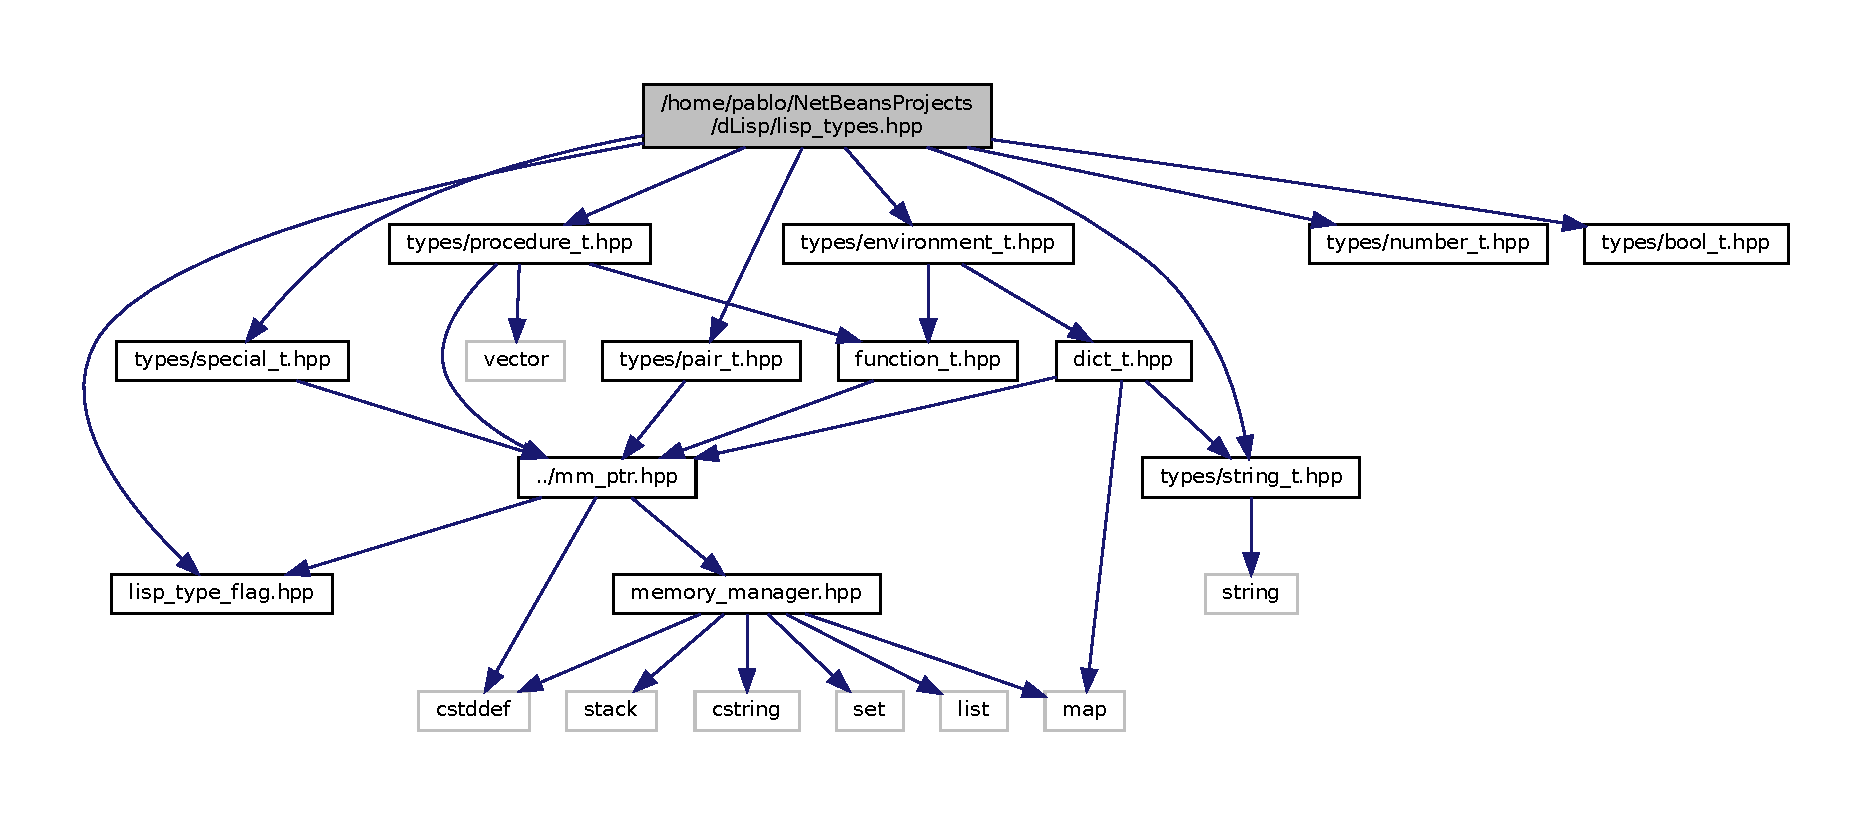
\includegraphics[width=350pt]{lisp__types_8hpp__incl}
\end{center}
\end{figure}
Граф файлов, в которые включается этот файл\+:
\nopagebreak
\begin{figure}[H]
\begin{center}
\leavevmode
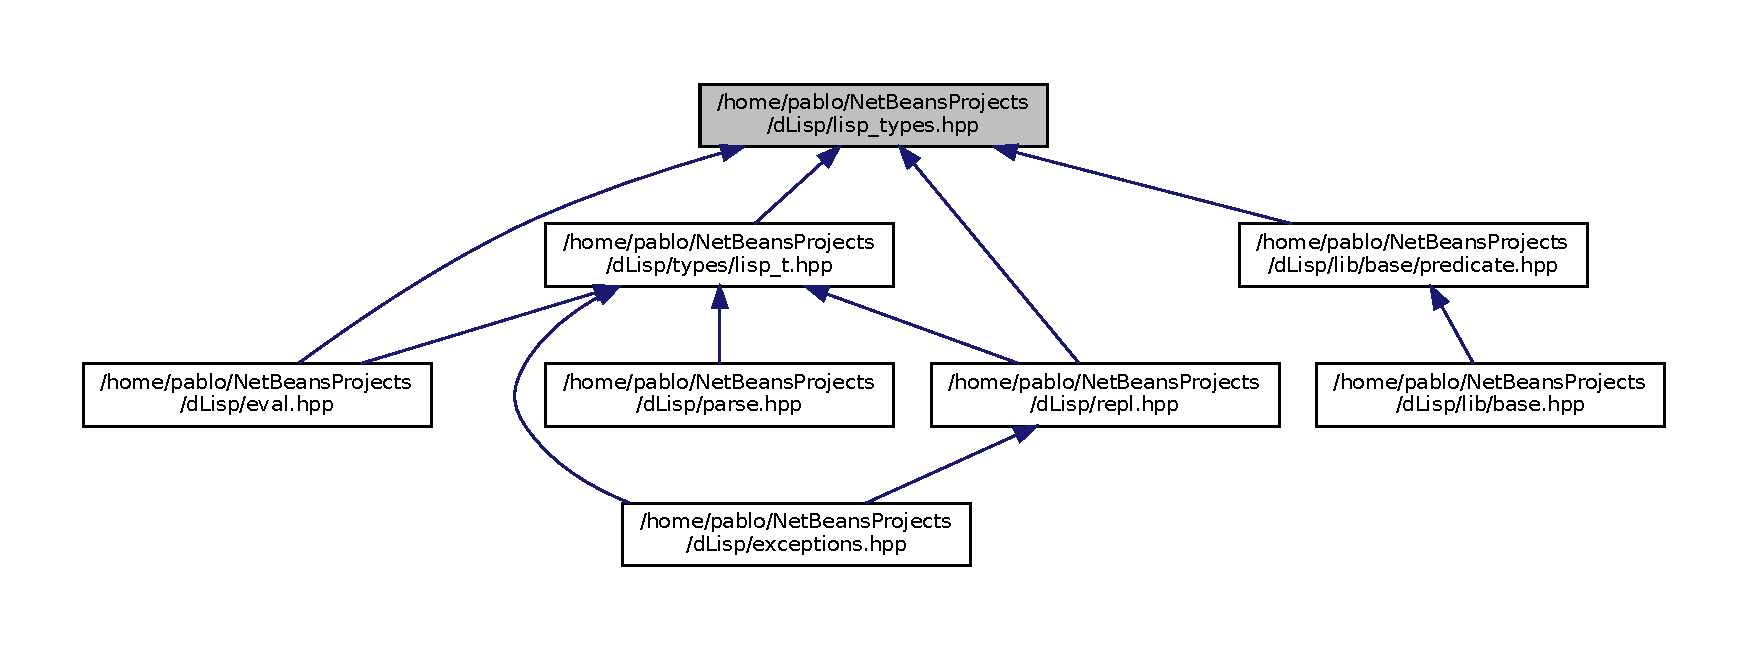
\includegraphics[width=350pt]{lisp__types_8hpp__dep__incl}
\end{center}
\end{figure}
\subsection*{Определения типов}
\begin{DoxyCompactItemize}
\item 
\mbox{\Hypertarget{lisp__types_8hpp_a543c62d3ca4ba3750602b9c6b11af1de}\label{lisp__types_8hpp_a543c62d3ca4ba3750602b9c6b11af1de}} 
using \mbox{\hyperlink{lisp__types_8hpp_a543c62d3ca4ba3750602b9c6b11af1de}{symbol\+\_\+t}} = \mbox{\hyperlink{classstring__t}{string\+\_\+t}}
\begin{DoxyCompactList}\small\item\em $<$ Класс lisp-\/типа символов \end{DoxyCompactList}\end{DoxyCompactItemize}


\subsection{Подробное описание}
\begin{DoxyAuthor}{Автор}
\+: Павел Коваленко 
\end{DoxyAuthor}
\begin{DoxyDate}{Дата}
27 июля 2018 г., 22\+:39 
\end{DoxyDate}

\hypertarget{bool__t_8hpp}{}\section{Файл /home/pablo/\+Net\+Beans\+Projects/d\+Lisp/types/bool\+\_\+t.hpp}
\label{bool__t_8hpp}\index{/home/pablo/\+Net\+Beans\+Projects/d\+Lisp/types/bool\+\_\+t.\+hpp@{/home/pablo/\+Net\+Beans\+Projects/d\+Lisp/types/bool\+\_\+t.\+hpp}}
Граф файлов, в которые включается этот файл\+:
\nopagebreak
\begin{figure}[H]
\begin{center}
\leavevmode
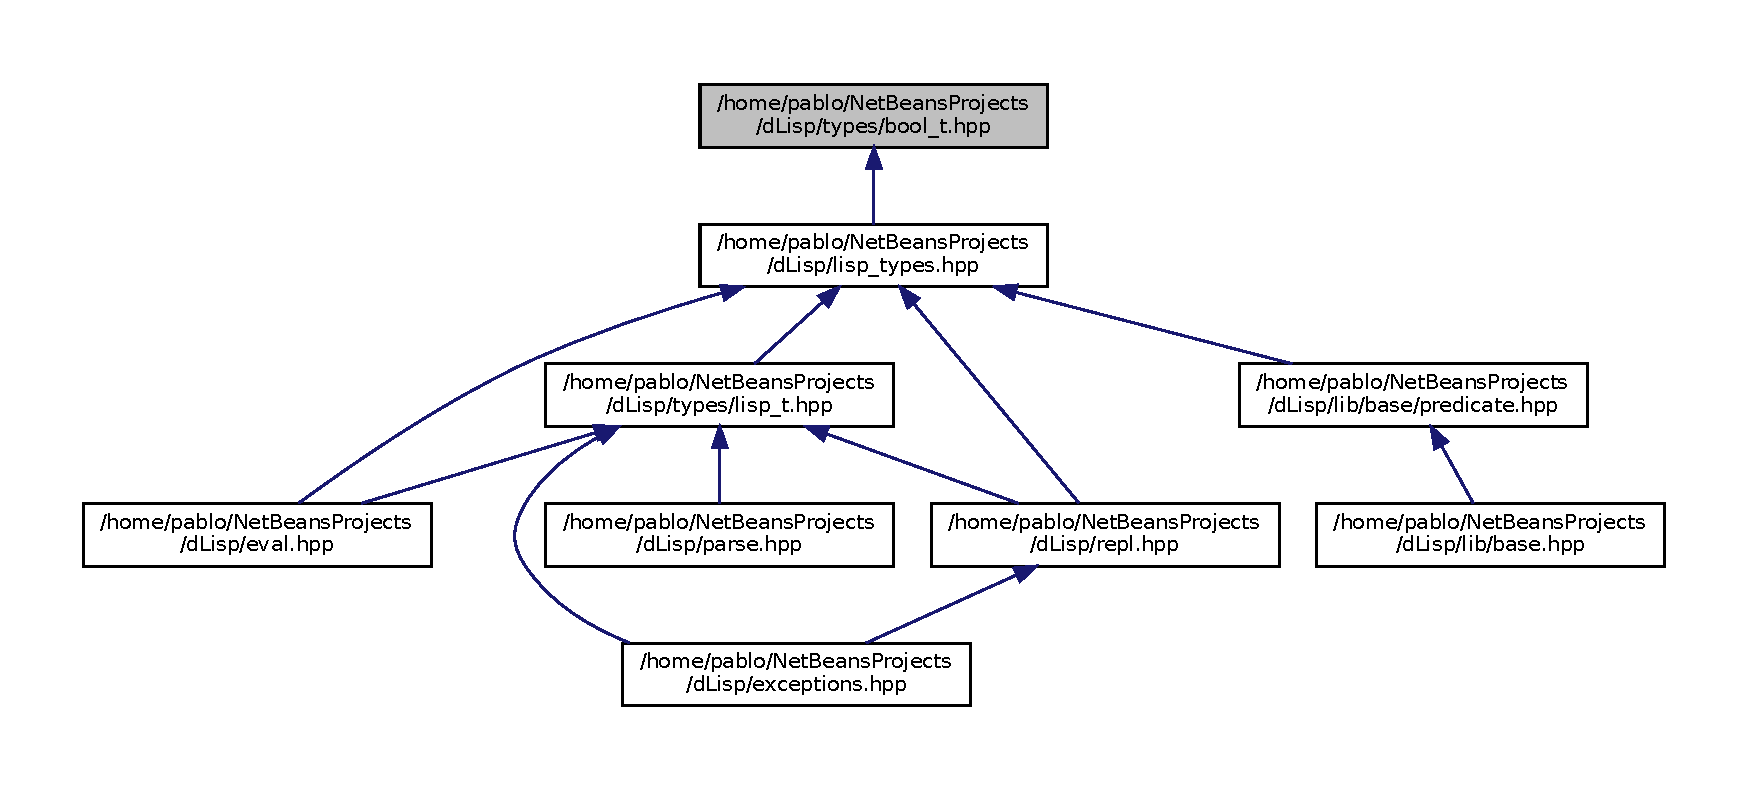
\includegraphics[width=350pt]{bool__t_8hpp__dep__incl}
\end{center}
\end{figure}
\subsection*{Классы}
\begin{DoxyCompactItemize}
\item 
class \mbox{\hyperlink{classbool__t}{bool\+\_\+t}}
\begin{DoxyCompactList}\small\item\em Класс булевого lisp-\/типа \end{DoxyCompactList}\end{DoxyCompactItemize}


\subsection{Подробное описание}
\begin{DoxyAuthor}{Автор}
\+: Павел Коваленко 
\end{DoxyAuthor}
\begin{DoxyDate}{Дата}
27 июля 2018 г., 22\+:07 
\end{DoxyDate}

\hypertarget{dict__t_8hpp}{}\section{Файл /home/pablo/\+Net\+Beans\+Projects/d\+Lisp/types/dict\+\_\+t.hpp}
\label{dict__t_8hpp}\index{/home/pablo/\+Net\+Beans\+Projects/d\+Lisp/types/dict\+\_\+t.\+hpp@{/home/pablo/\+Net\+Beans\+Projects/d\+Lisp/types/dict\+\_\+t.\+hpp}}
{\ttfamily \#include $<$map$>$}\newline
{\ttfamily \#include \char`\"{}string\+\_\+t.\+hpp\char`\"{}}\newline
{\ttfamily \#include \char`\"{}../mm\+\_\+ptr.\+hpp\char`\"{}}\newline
Граф включаемых заголовочных файлов для dict\+\_\+t.\+hpp\+:
\nopagebreak
\begin{figure}[H]
\begin{center}
\leavevmode
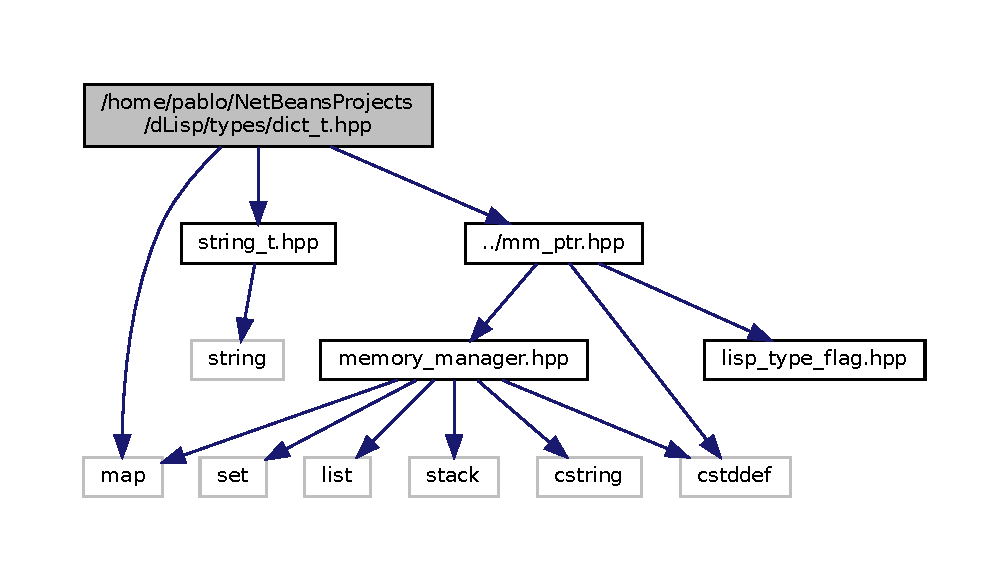
\includegraphics[width=350pt]{dict__t_8hpp__incl}
\end{center}
\end{figure}
Граф файлов, в которые включается этот файл\+:
\nopagebreak
\begin{figure}[H]
\begin{center}
\leavevmode
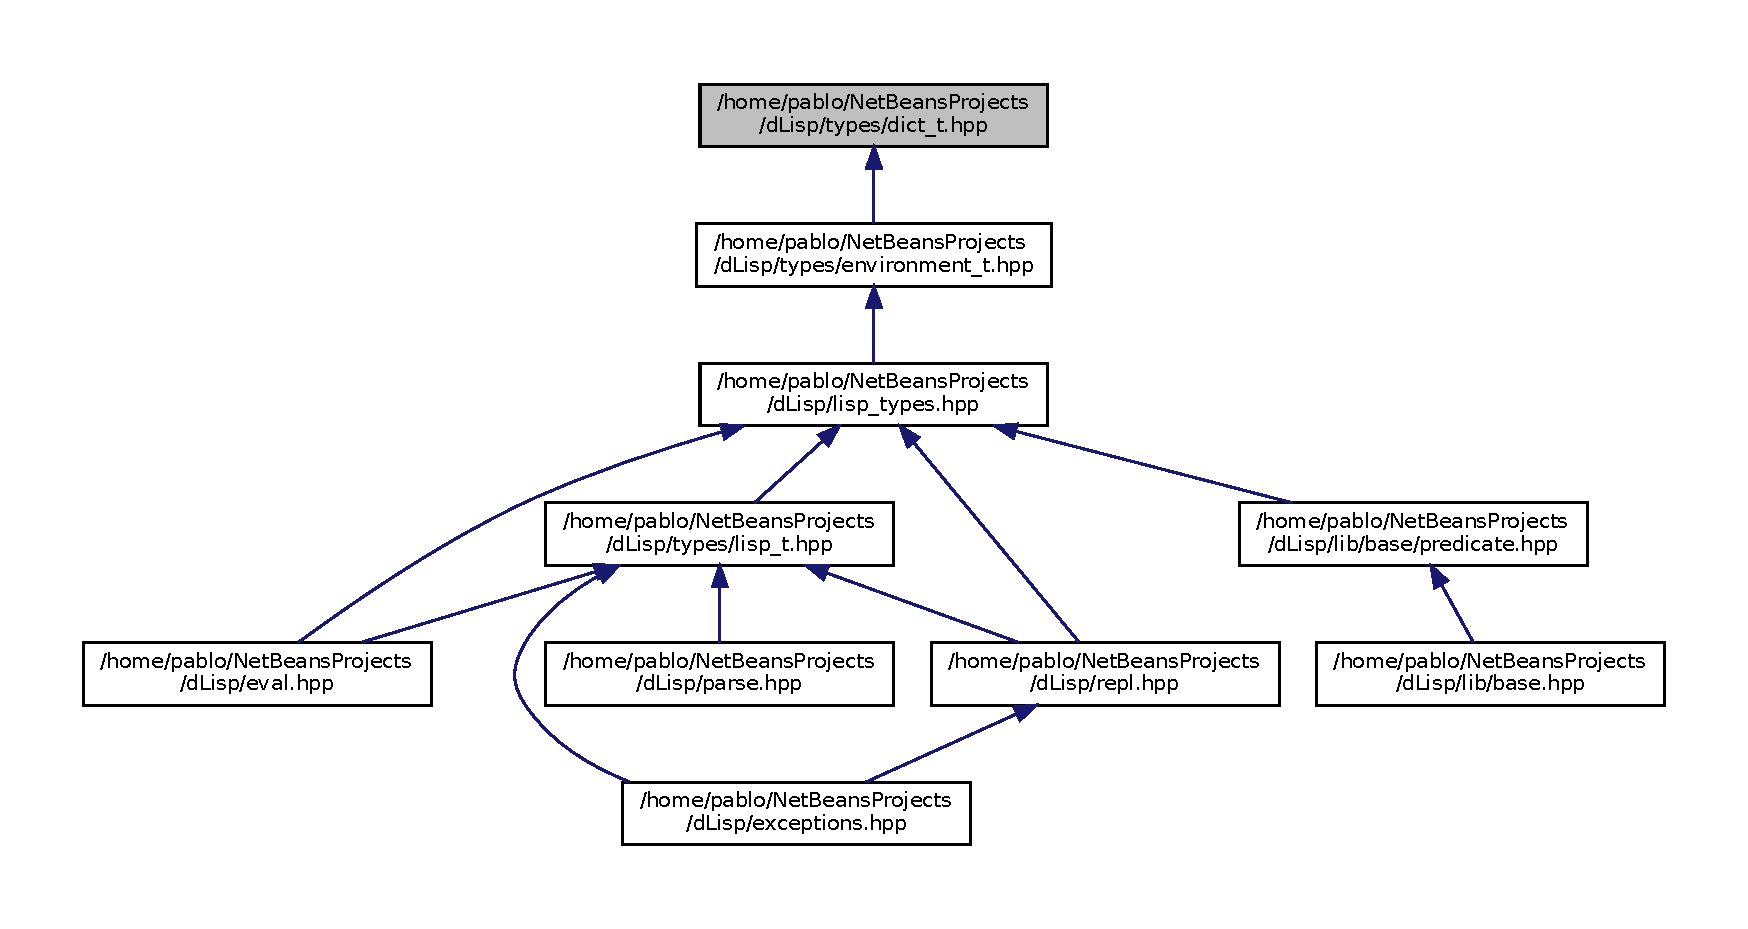
\includegraphics[width=350pt]{dict__t_8hpp__dep__incl}
\end{center}
\end{figure}
\subsection*{Определения типов}
\begin{DoxyCompactItemize}
\item 
\mbox{\Hypertarget{dict__t_8hpp_a543c62d3ca4ba3750602b9c6b11af1de}\label{dict__t_8hpp_a543c62d3ca4ba3750602b9c6b11af1de}} 
using {\bfseries symbol\+\_\+t} = \mbox{\hyperlink{classstring__t}{string\+\_\+t}}
\item 
\mbox{\Hypertarget{dict__t_8hpp_a56fdc8959ea1ff56de0242f602b1e649}\label{dict__t_8hpp_a56fdc8959ea1ff56de0242f602b1e649}} 
using \mbox{\hyperlink{dict__t_8hpp_a56fdc8959ea1ff56de0242f602b1e649}{dict\+\_\+t}} = std\+::map$<$ \mbox{\hyperlink{lisp__types_8hpp_a543c62d3ca4ba3750602b9c6b11af1de}{symbol\+\_\+t}}, \mbox{\hyperlink{classmm__ptr}{obj\+\_\+ptr}} $>$
\begin{DoxyCompactList}\small\item\em Отвечает за хранение пар символ-\/значение в октужениях \end{DoxyCompactList}\end{DoxyCompactItemize}


\subsection{Подробное описание}
\begin{DoxyAuthor}{Автор}
\+: Павел Коваленко 
\end{DoxyAuthor}
\begin{DoxyDate}{Дата}
23 июля 2018 г., 22\+:29 
\end{DoxyDate}

\hypertarget{environment__t_8hpp}{}\section{Файл /home/pablo/\+Net\+Beans\+Projects/d\+Lisp/types/environment\+\_\+t.hpp}
\label{environment__t_8hpp}\index{/home/pablo/\+Net\+Beans\+Projects/d\+Lisp/types/environment\+\_\+t.\+hpp@{/home/pablo/\+Net\+Beans\+Projects/d\+Lisp/types/environment\+\_\+t.\+hpp}}
{\ttfamily \#include \char`\"{}function\+\_\+t.\+hpp\char`\"{}}\newline
{\ttfamily \#include \char`\"{}dict\+\_\+t.\+hpp\char`\"{}}\newline
Граф включаемых заголовочных файлов для environment\+\_\+t.\+hpp\+:
\nopagebreak
\begin{figure}[H]
\begin{center}
\leavevmode
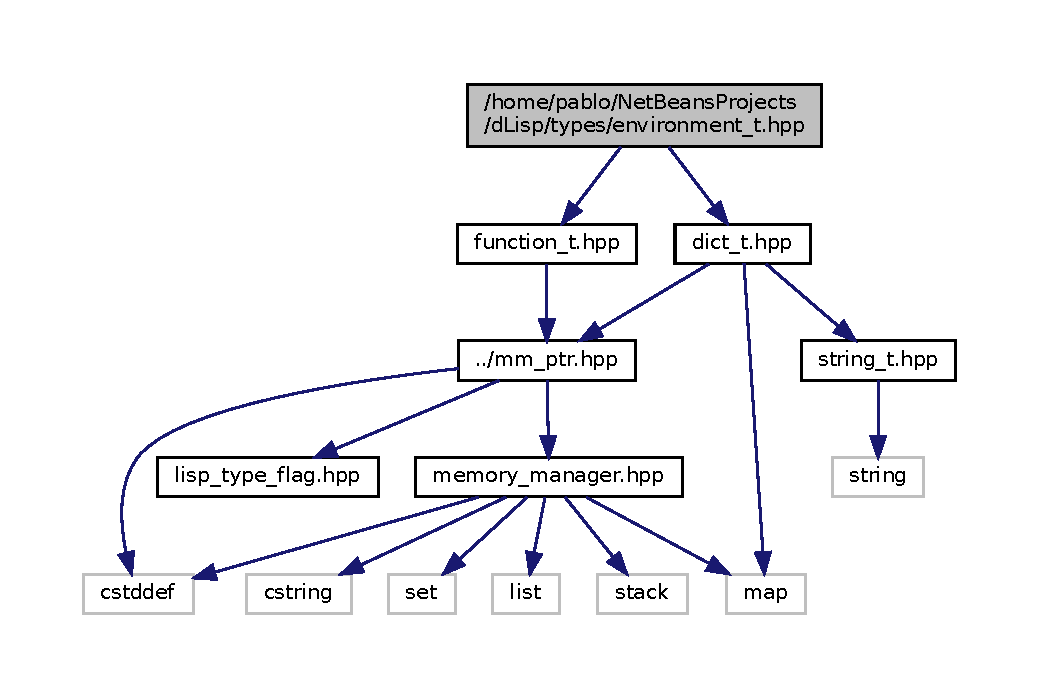
\includegraphics[width=350pt]{environment__t_8hpp__incl}
\end{center}
\end{figure}
Граф файлов, в которые включается этот файл\+:
\nopagebreak
\begin{figure}[H]
\begin{center}
\leavevmode
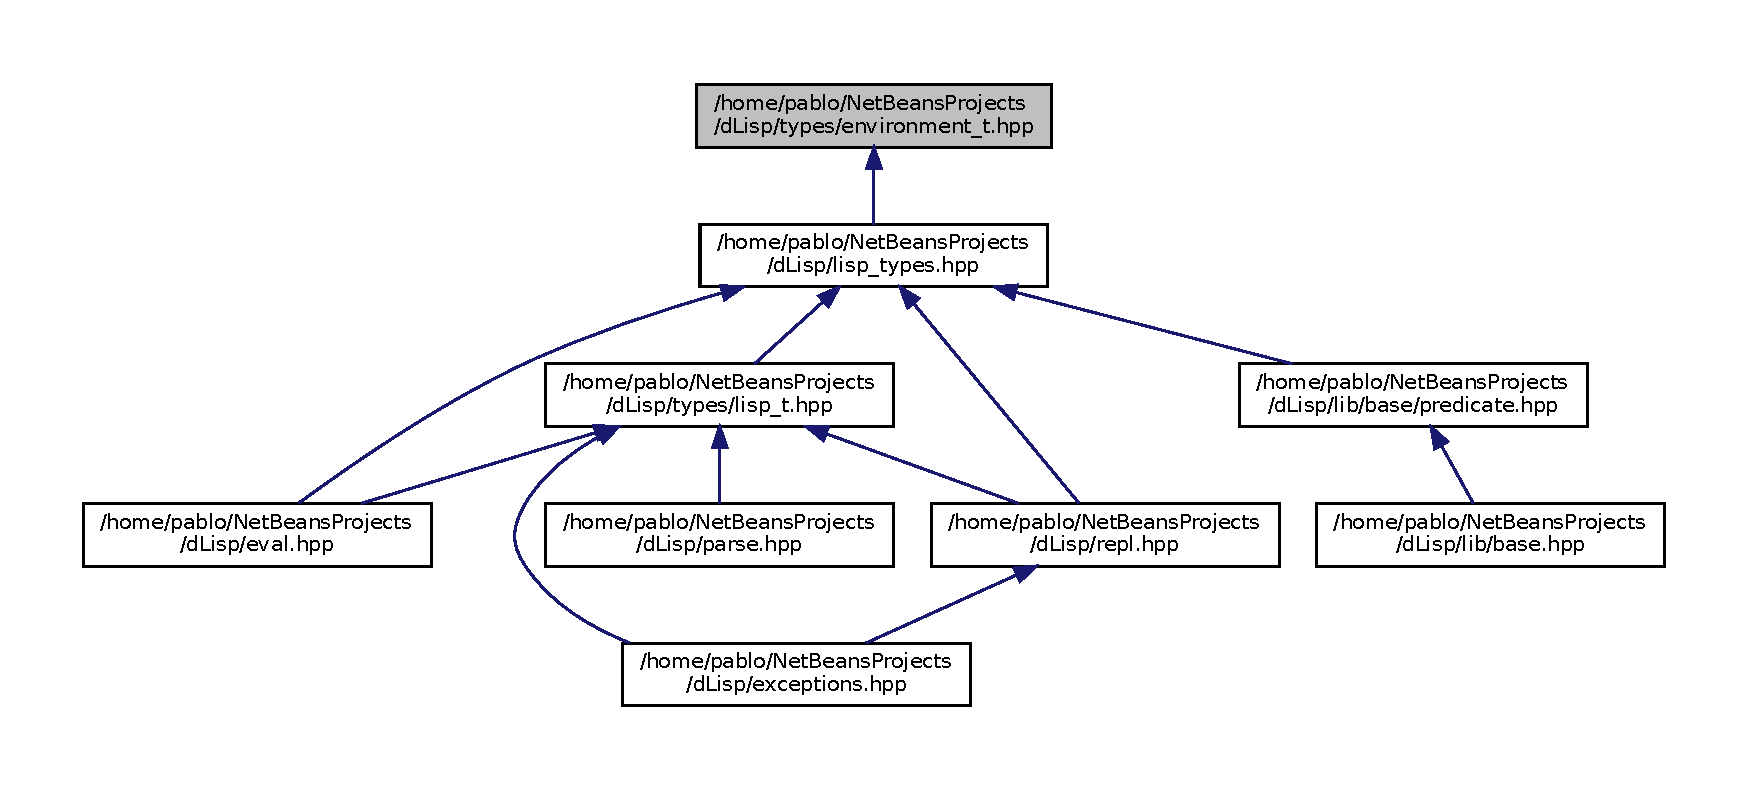
\includegraphics[width=350pt]{environment__t_8hpp__dep__incl}
\end{center}
\end{figure}
\subsection*{Классы}
\begin{DoxyCompactItemize}
\item 
class \mbox{\hyperlink{classenvironment__t}{environment\+\_\+t}}
\begin{DoxyCompactList}\small\item\em Класс lisp-\/типа окружения \end{DoxyCompactList}\end{DoxyCompactItemize}
\subsection*{Функции}
\begin{DoxyCompactItemize}
\item 
\mbox{\hyperlink{classmm__ptr}{env\+\_\+ptr}} \mbox{\hyperlink{environment__t_8hpp_a6d895f270ea506101c8ef446e1f7edea}{make\+\_\+global\+\_\+env}} ()
\begin{DoxyCompactList}\small\item\em Создает объект глобального окружения \end{DoxyCompactList}\end{DoxyCompactItemize}


\subsection{Подробное описание}
\begin{DoxyAuthor}{Автор}
\+: Павел Коваленко 
\end{DoxyAuthor}
\begin{DoxyDate}{Дата}
23 июля 2018 г., 22\+:26 
\end{DoxyDate}


\subsection{Функции}
\mbox{\Hypertarget{environment__t_8hpp_a6d895f270ea506101c8ef446e1f7edea}\label{environment__t_8hpp_a6d895f270ea506101c8ef446e1f7edea}} 
\index{environment\+\_\+t.\+hpp@{environment\+\_\+t.\+hpp}!make\+\_\+global\+\_\+env@{make\+\_\+global\+\_\+env}}
\index{make\+\_\+global\+\_\+env@{make\+\_\+global\+\_\+env}!environment\+\_\+t.\+hpp@{environment\+\_\+t.\+hpp}}
\subsubsection{\texorpdfstring{make\+\_\+global\+\_\+env()}{make\_global\_env()}}
{\footnotesize\ttfamily \mbox{\hyperlink{classmm__ptr}{env\+\_\+ptr}} make\+\_\+global\+\_\+env (\begin{DoxyParamCaption}{ }\end{DoxyParamCaption})}



Создает объект глобального окружения 

\begin{DoxyReturn}{Возвращает}
Новый объект глобального окружения
\end{DoxyReturn}
Создает и возвращает новый объект глобального окружения к которому подключены некоторые базовые библиотеки 
\hypertarget{number__t_8hpp}{}\section{Файл /home/pablo/\+Net\+Beans\+Projects/d\+Lisp/types/number\+\_\+t.hpp}
\label{number__t_8hpp}\index{/home/pablo/\+Net\+Beans\+Projects/d\+Lisp/types/number\+\_\+t.\+hpp@{/home/pablo/\+Net\+Beans\+Projects/d\+Lisp/types/number\+\_\+t.\+hpp}}
Граф файлов, в которые включается этот файл\+:
\nopagebreak
\begin{figure}[H]
\begin{center}
\leavevmode
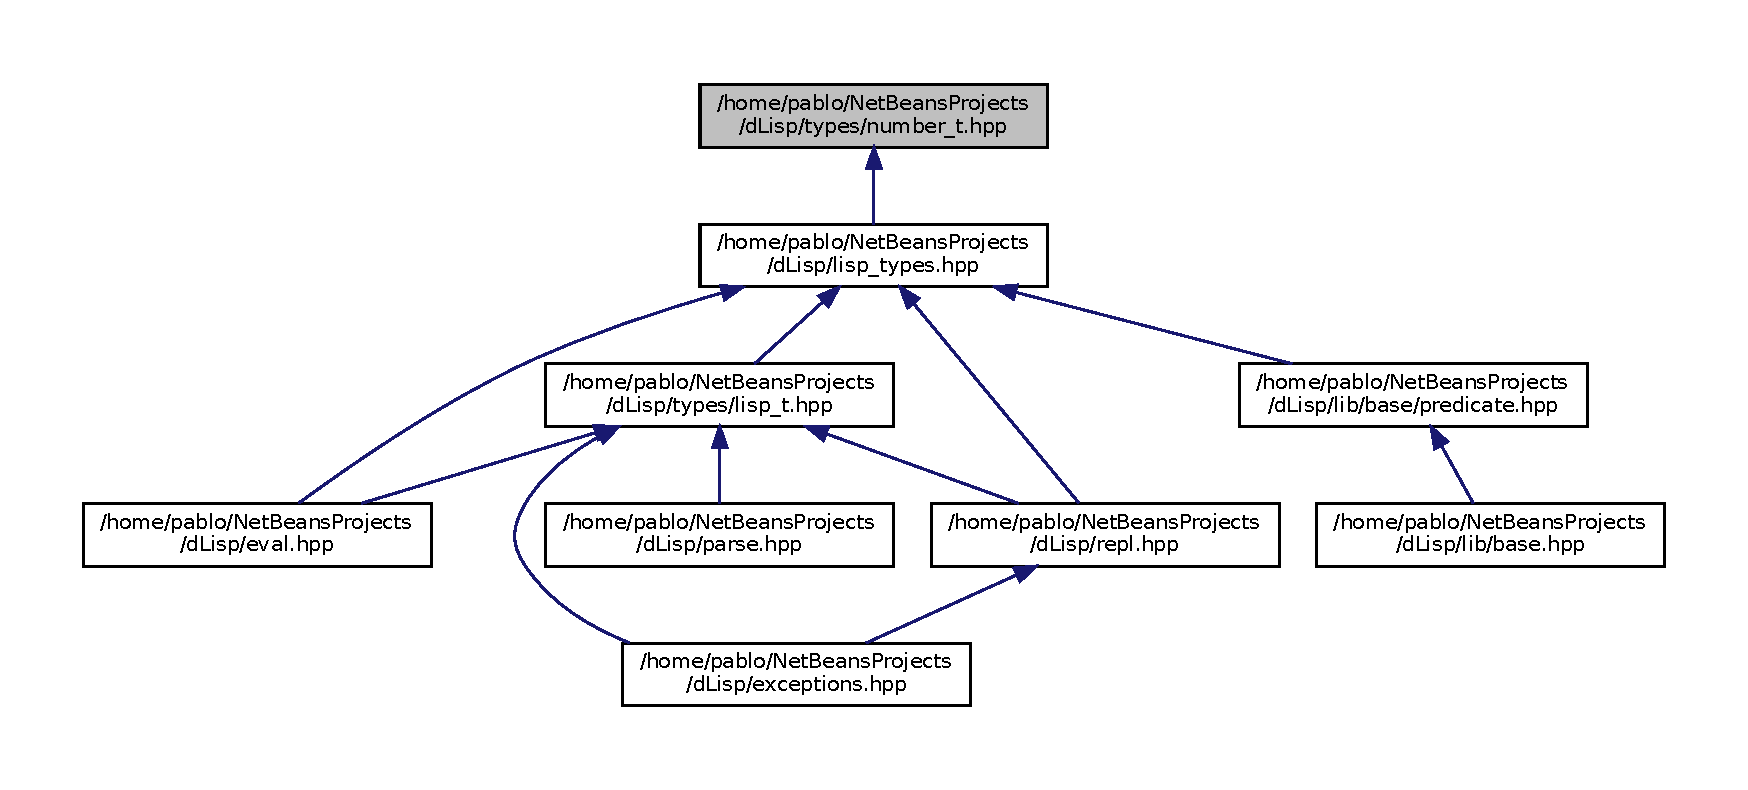
\includegraphics[width=350pt]{number__t_8hpp__dep__incl}
\end{center}
\end{figure}
\subsection*{Классы}
\begin{DoxyCompactItemize}
\item 
class \mbox{\hyperlink{classnumber__t}{number\+\_\+t}}
\begin{DoxyCompactList}\small\item\em Класс lisp-\/типа чисел \end{DoxyCompactList}\end{DoxyCompactItemize}
\subsection*{Перечисления}
\begin{DoxyCompactItemize}
\item 
enum \mbox{\hyperlink{number__t_8hpp_a9c37ed0386636f462116b6e8d1fd8312}{number\+\_\+type\+\_\+flag}} \+: bool \{ \mbox{\hyperlink{number__t_8hpp_a9c37ed0386636f462116b6e8d1fd8312a5249c7b902d0b707d48b0c769a520db3}{T\+\_\+\+R\+E\+AL}}, 
\mbox{\hyperlink{number__t_8hpp_a9c37ed0386636f462116b6e8d1fd8312aa30cbb0eb56b7263a35f9d6643e12c83}{T\+\_\+\+I\+NT}}
 \}
\begin{DoxyCompactList}\small\item\em Флаги типов чисел \end{DoxyCompactList}\end{DoxyCompactItemize}
\subsection*{Переменные}
\begin{DoxyCompactItemize}
\item 
\mbox{\Hypertarget{number__t_8hpp_ac29df3dcbefa1ce189e5990bde994025}\label{number__t_8hpp_ac29df3dcbefa1ce189e5990bde994025}} 
const double {\bfseries epsilon} = 0.\+000000001
\end{DoxyCompactItemize}


\subsection{Подробное описание}
\begin{DoxyAuthor}{Автор}
\+: Павел Коваленко 
\end{DoxyAuthor}
\begin{DoxyDate}{Дата}
23 июля 2018 г., 22\+:15 
\end{DoxyDate}


\subsection{Перечисления}
\mbox{\Hypertarget{number__t_8hpp_a9c37ed0386636f462116b6e8d1fd8312}\label{number__t_8hpp_a9c37ed0386636f462116b6e8d1fd8312}} 
\index{number\+\_\+t.\+hpp@{number\+\_\+t.\+hpp}!number\+\_\+type\+\_\+flag@{number\+\_\+type\+\_\+flag}}
\index{number\+\_\+type\+\_\+flag@{number\+\_\+type\+\_\+flag}!number\+\_\+t.\+hpp@{number\+\_\+t.\+hpp}}
\subsubsection{\texorpdfstring{number\+\_\+type\+\_\+flag}{number\_type\_flag}}
{\footnotesize\ttfamily enum \mbox{\hyperlink{number__t_8hpp_a9c37ed0386636f462116b6e8d1fd8312}{number\+\_\+type\+\_\+flag}} \+: bool}



Флаги типов чисел 

\begin{DoxyEnumFields}{Элементы перечислений}
\raisebox{\heightof{T}}[0pt][0pt]{\index{T\+\_\+\+R\+E\+AL@{T\+\_\+\+R\+E\+AL}!number\+\_\+t.\+hpp@{number\+\_\+t.\+hpp}}\index{number\+\_\+t.\+hpp@{number\+\_\+t.\+hpp}!T\+\_\+\+R\+E\+AL@{T\+\_\+\+R\+E\+AL}}}\mbox{\Hypertarget{number__t_8hpp_a9c37ed0386636f462116b6e8d1fd8312a5249c7b902d0b707d48b0c769a520db3}\label{number__t_8hpp_a9c37ed0386636f462116b6e8d1fd8312a5249c7b902d0b707d48b0c769a520db3}} 
T\+\_\+\+R\+E\+AL&Вещественное число \\
\hline

\raisebox{\heightof{T}}[0pt][0pt]{\index{T\+\_\+\+I\+NT@{T\+\_\+\+I\+NT}!number\+\_\+t.\+hpp@{number\+\_\+t.\+hpp}}\index{number\+\_\+t.\+hpp@{number\+\_\+t.\+hpp}!T\+\_\+\+I\+NT@{T\+\_\+\+I\+NT}}}\mbox{\Hypertarget{number__t_8hpp_a9c37ed0386636f462116b6e8d1fd8312aa30cbb0eb56b7263a35f9d6643e12c83}\label{number__t_8hpp_a9c37ed0386636f462116b6e8d1fd8312aa30cbb0eb56b7263a35f9d6643e12c83}} 
T\+\_\+\+I\+NT&Целое число \\
\hline

\end{DoxyEnumFields}

\hypertarget{pair__t_8hpp}{}\section{Файл /home/pablo/\+Net\+Beans\+Projects/d\+Lisp/types/pair\+\_\+t.hpp}
\label{pair__t_8hpp}\index{/home/pablo/\+Net\+Beans\+Projects/d\+Lisp/types/pair\+\_\+t.\+hpp@{/home/pablo/\+Net\+Beans\+Projects/d\+Lisp/types/pair\+\_\+t.\+hpp}}
{\ttfamily \#include \char`\"{}../mm\+\_\+ptr.\+hpp\char`\"{}}\newline
Граф включаемых заголовочных файлов для pair\+\_\+t.\+hpp\+:
\nopagebreak
\begin{figure}[H]
\begin{center}
\leavevmode
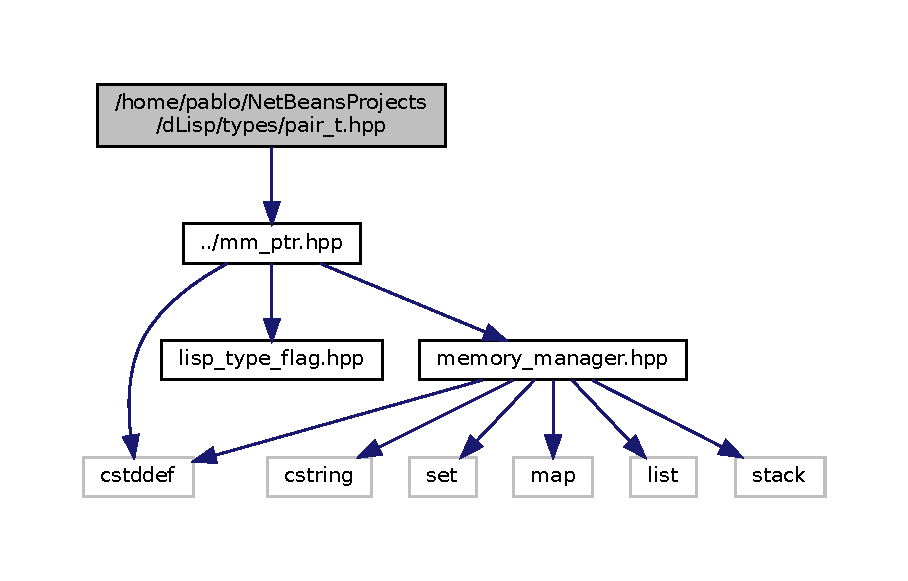
\includegraphics[width=350pt]{pair__t_8hpp__incl}
\end{center}
\end{figure}
Граф файлов, в которые включается этот файл\+:
\nopagebreak
\begin{figure}[H]
\begin{center}
\leavevmode
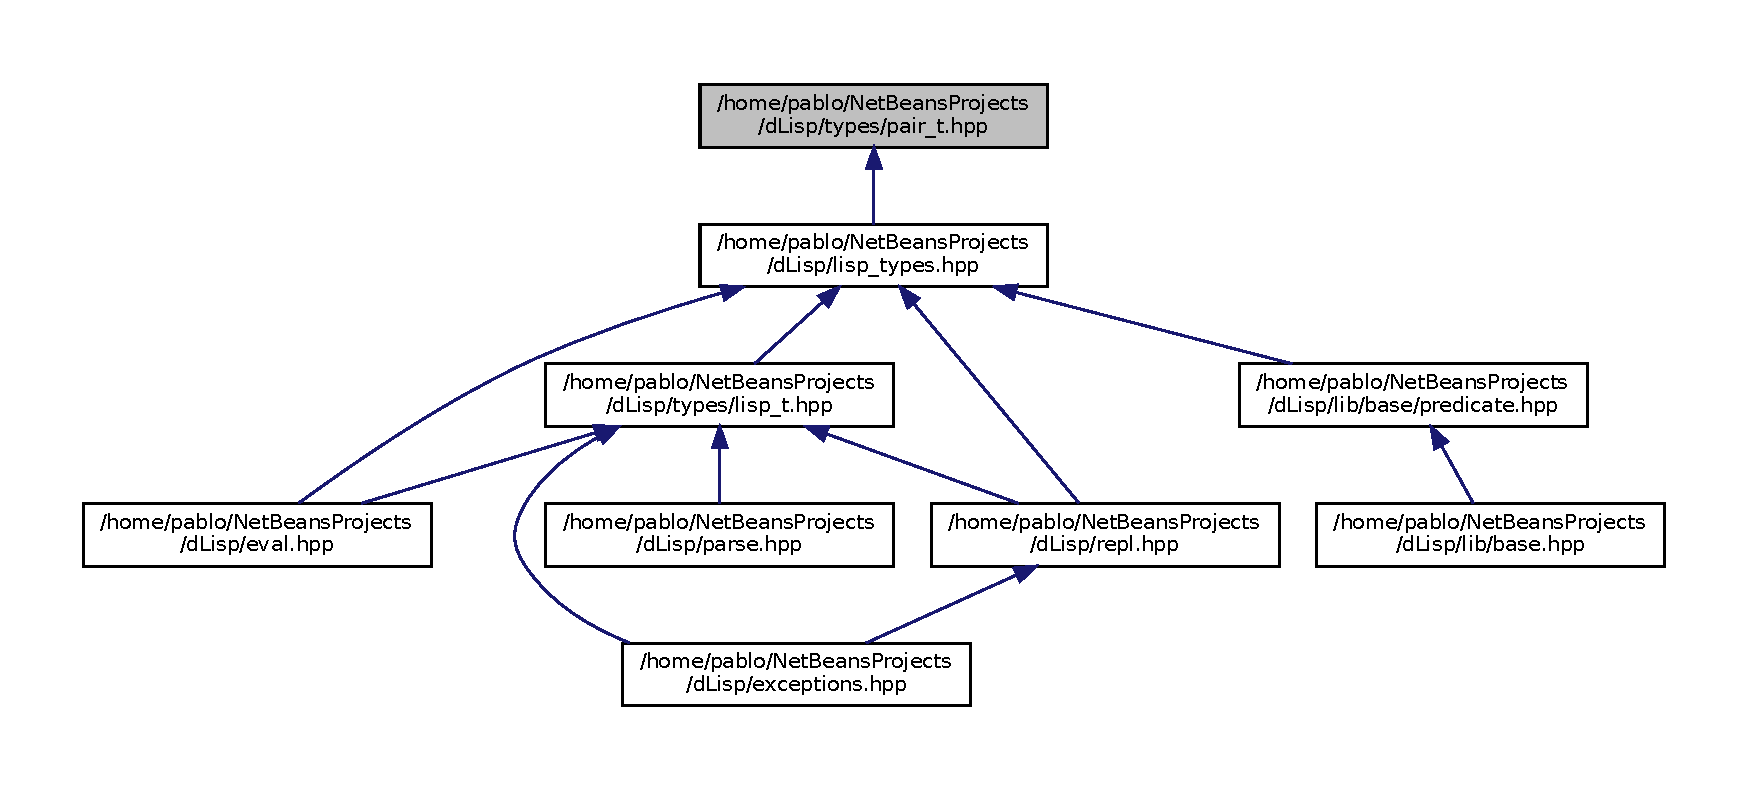
\includegraphics[width=350pt]{pair__t_8hpp__dep__incl}
\end{center}
\end{figure}
\subsection*{Классы}
\begin{DoxyCompactItemize}
\item 
class \mbox{\hyperlink{classpair__t}{pair\+\_\+t}}
\begin{DoxyCompactList}\small\item\em Класс lisp-\/типа пар \end{DoxyCompactList}\end{DoxyCompactItemize}


\subsection{Подробное описание}
\begin{DoxyAuthor}{Автор}
\+: Павел Коваленко 
\end{DoxyAuthor}
\begin{DoxyDate}{Дата}
27 июля 2018 г., 22\+:00 
\end{DoxyDate}

\hypertarget{procedure__t_8hpp}{}\section{Файл /home/pablo/\+Net\+Beans\+Projects/d\+Lisp/types/procedure\+\_\+t.hpp}
\label{procedure__t_8hpp}\index{/home/pablo/\+Net\+Beans\+Projects/d\+Lisp/types/procedure\+\_\+t.\+hpp@{/home/pablo/\+Net\+Beans\+Projects/d\+Lisp/types/procedure\+\_\+t.\+hpp}}
{\ttfamily \#include \char`\"{}function\+\_\+t.\+hpp\char`\"{}}\newline
{\ttfamily \#include \char`\"{}../mm\+\_\+ptr.\+hpp\char`\"{}}\newline
{\ttfamily \#include $<$vector$>$}\newline
Граф включаемых заголовочных файлов для procedure\+\_\+t.\+hpp\+:
\nopagebreak
\begin{figure}[H]
\begin{center}
\leavevmode
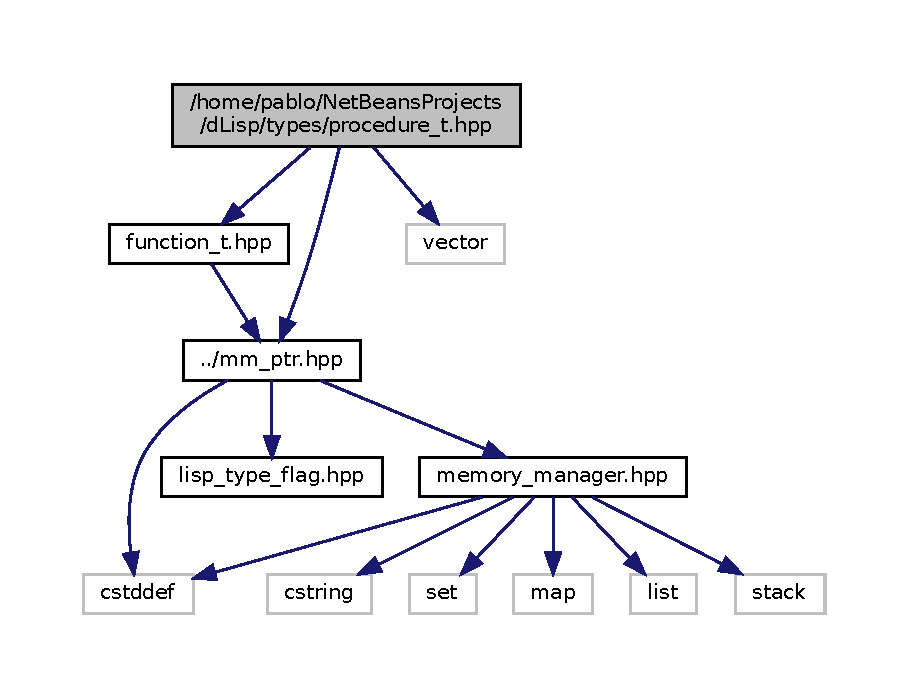
\includegraphics[width=350pt]{procedure__t_8hpp__incl}
\end{center}
\end{figure}
Граф файлов, в которые включается этот файл\+:
\nopagebreak
\begin{figure}[H]
\begin{center}
\leavevmode
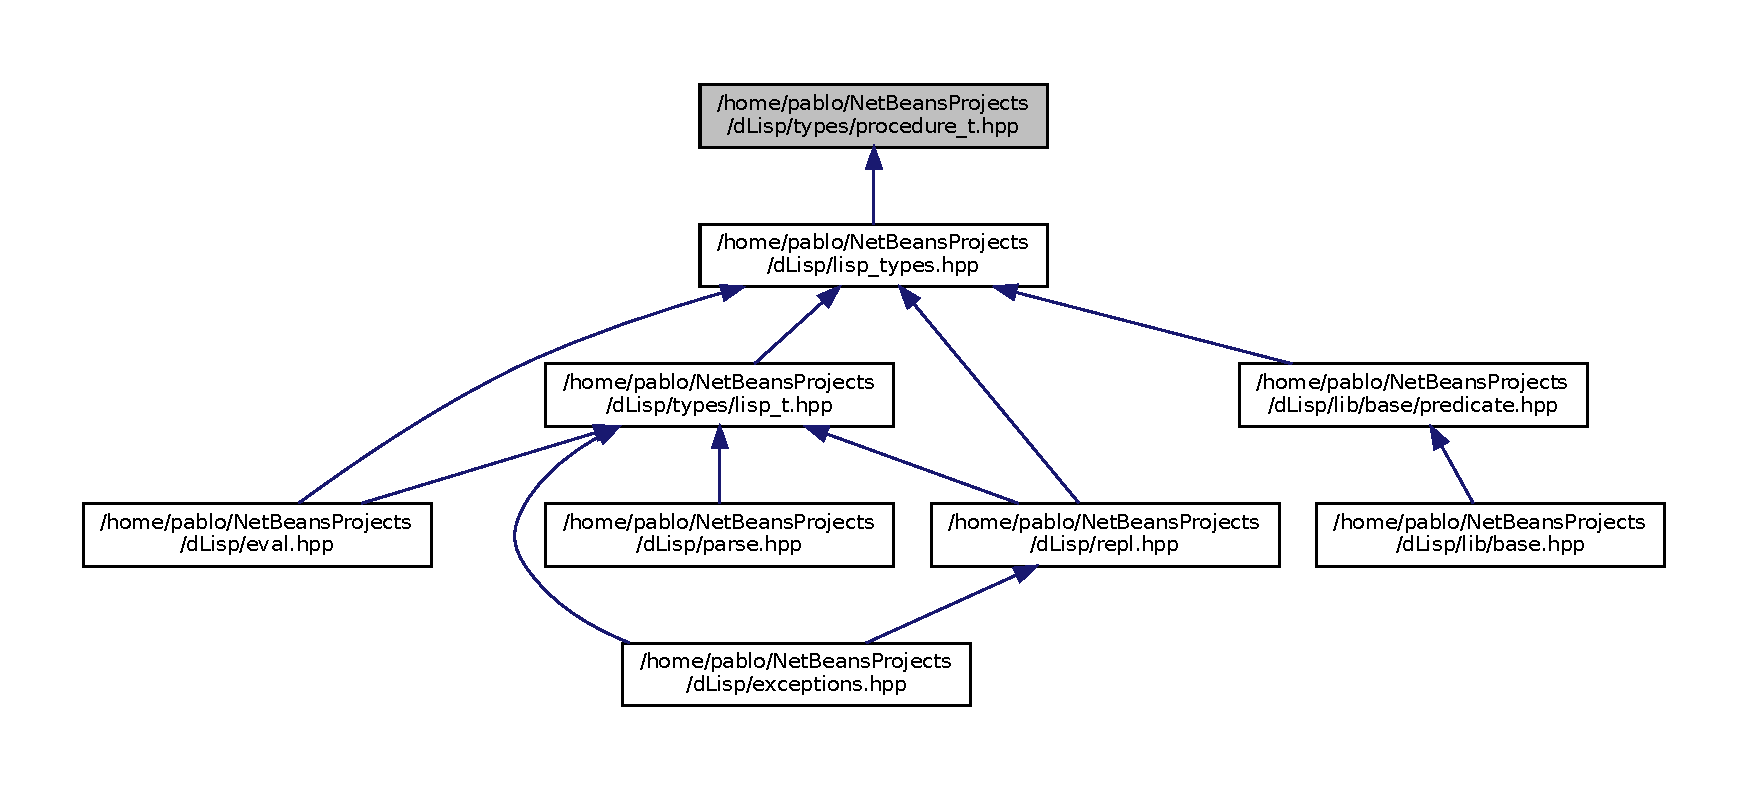
\includegraphics[width=350pt]{procedure__t_8hpp__dep__incl}
\end{center}
\end{figure}
\subsection*{Классы}
\begin{DoxyCompactItemize}
\item 
class \mbox{\hyperlink{classprocedure__t}{procedure\+\_\+t}}
\begin{DoxyCompactList}\small\item\em Класс lisp-\/типа процедуры \end{DoxyCompactList}\end{DoxyCompactItemize}


\subsection{Подробное описание}
\begin{DoxyAuthor}{Автор}
\+: Павел Коваленко 
\end{DoxyAuthor}
\begin{DoxyDate}{Дата}
23 июля 2018 г., 22\+:32 
\end{DoxyDate}

\hypertarget{special__t_8hpp}{}\section{Файл /home/pablo/\+Net\+Beans\+Projects/d\+Lisp/types/special\+\_\+t.hpp}
\label{special__t_8hpp}\index{/home/pablo/\+Net\+Beans\+Projects/d\+Lisp/types/special\+\_\+t.\+hpp@{/home/pablo/\+Net\+Beans\+Projects/d\+Lisp/types/special\+\_\+t.\+hpp}}
{\ttfamily \#include \char`\"{}../mm\+\_\+ptr.\+hpp\char`\"{}}\newline
Граф включаемых заголовочных файлов для special\+\_\+t.\+hpp\+:
\nopagebreak
\begin{figure}[H]
\begin{center}
\leavevmode
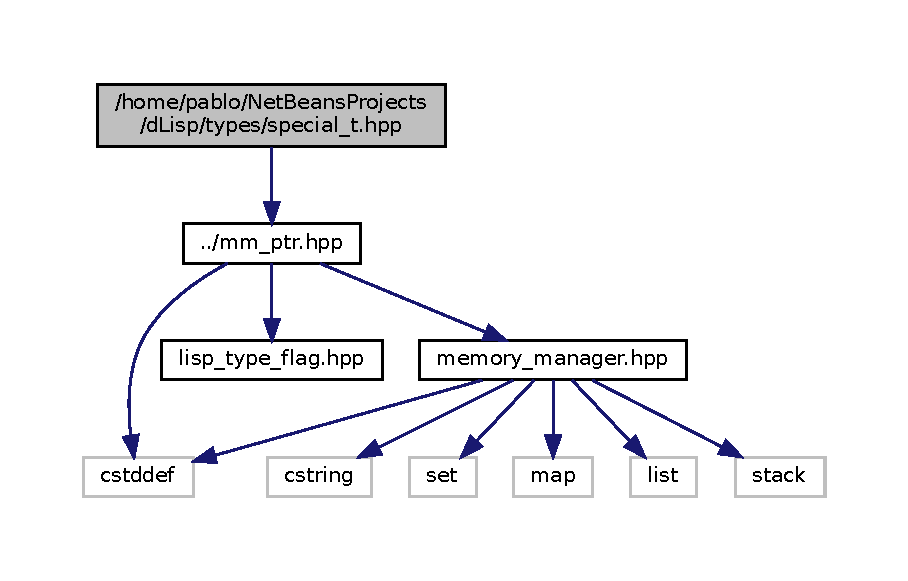
\includegraphics[width=350pt]{special__t_8hpp__incl}
\end{center}
\end{figure}
Граф файлов, в которые включается этот файл\+:
\nopagebreak
\begin{figure}[H]
\begin{center}
\leavevmode
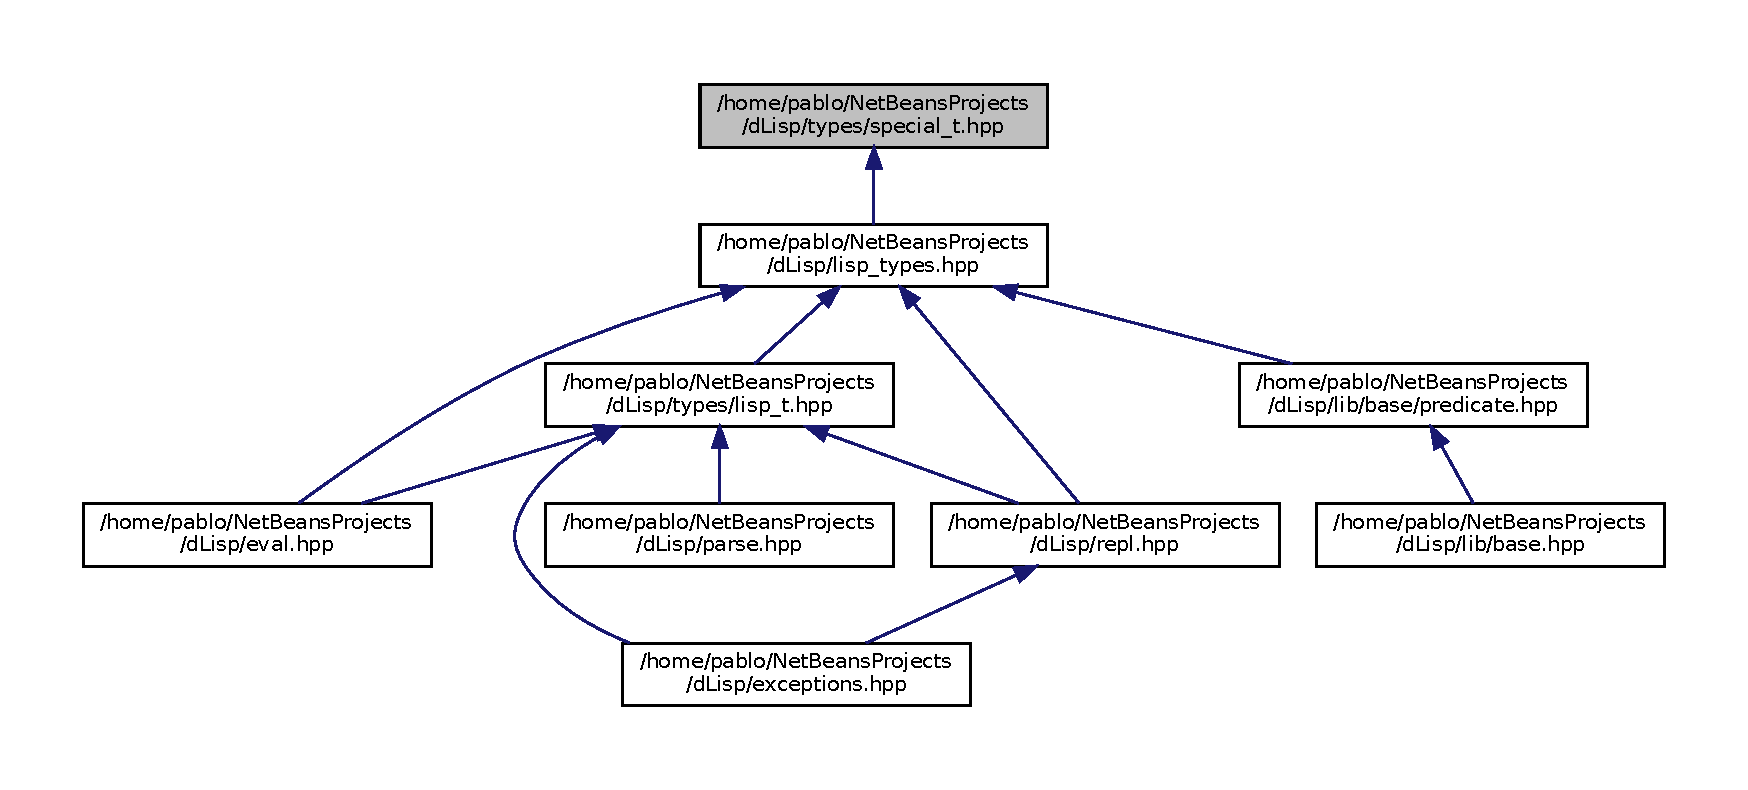
\includegraphics[width=350pt]{special__t_8hpp__dep__incl}
\end{center}
\end{figure}
\subsection*{Классы}
\begin{DoxyCompactItemize}
\item 
class \mbox{\hyperlink{classspecial__t}{special\+\_\+t}}
\begin{DoxyCompactList}\small\item\em Класс lisp-\/типа специальных значение \end{DoxyCompactList}\end{DoxyCompactItemize}
\subsection*{Перечисления}
\begin{DoxyCompactItemize}
\item 
enum \mbox{\hyperlink{special__t_8hpp_af80c2ea5ebf91ef19f47fd2e190d7149}{special\+\_\+type\+\_\+flag}} \+: char \{ \mbox{\hyperlink{special__t_8hpp_af80c2ea5ebf91ef19f47fd2e190d7149a632fa39438c1676b435ec43e6a0f9647}{U\+N\+D\+EF}}, 
\mbox{\hyperlink{special__t_8hpp_af80c2ea5ebf91ef19f47fd2e190d7149a2e6059d72d8fde88f3127eb147e4eff8}{I\+NF}}, 
\mbox{\hyperlink{special__t_8hpp_af80c2ea5ebf91ef19f47fd2e190d7149a75bee44ae49a0cecbbab062cc74f53a7}{N\+AN}}
 \}
\begin{DoxyCompactList}\small\item\em Флаги типов специальных объектов \end{DoxyCompactList}\end{DoxyCompactItemize}
\subsection*{Функции}
\begin{DoxyCompactItemize}
\item 
\mbox{\Hypertarget{special__t_8hpp_a7e0c41c0e60ca07d6049c2c021477be1}\label{special__t_8hpp_a7e0c41c0e60ca07d6049c2c021477be1}} 
\mbox{\hyperlink{classmm__ptr}{obj\+\_\+ptr}} \mbox{\hyperlink{special__t_8hpp_a7e0c41c0e60ca07d6049c2c021477be1}{undefined}} ()
\begin{DoxyCompactList}\small\item\em Создает объект -\/ неопределенное значение \end{DoxyCompactList}\end{DoxyCompactItemize}


\subsection{Подробное описание}
\begin{DoxyAuthor}{Автор}
\+: Павел Коваленко 
\end{DoxyAuthor}
\begin{DoxyDate}{Дата}
28 июля 2018 г., 17\+:59 
\end{DoxyDate}


\subsection{Перечисления}
\mbox{\Hypertarget{special__t_8hpp_af80c2ea5ebf91ef19f47fd2e190d7149}\label{special__t_8hpp_af80c2ea5ebf91ef19f47fd2e190d7149}} 
\index{special\+\_\+t.\+hpp@{special\+\_\+t.\+hpp}!special\+\_\+type\+\_\+flag@{special\+\_\+type\+\_\+flag}}
\index{special\+\_\+type\+\_\+flag@{special\+\_\+type\+\_\+flag}!special\+\_\+t.\+hpp@{special\+\_\+t.\+hpp}}
\subsubsection{\texorpdfstring{special\+\_\+type\+\_\+flag}{special\_type\_flag}}
{\footnotesize\ttfamily enum \mbox{\hyperlink{special__t_8hpp_af80c2ea5ebf91ef19f47fd2e190d7149}{special\+\_\+type\+\_\+flag}} \+: char}



Флаги типов специальных объектов 

\begin{DoxyEnumFields}{Элементы перечислений}
\raisebox{\heightof{T}}[0pt][0pt]{\index{U\+N\+D\+EF@{U\+N\+D\+EF}!special\+\_\+t.\+hpp@{special\+\_\+t.\+hpp}}\index{special\+\_\+t.\+hpp@{special\+\_\+t.\+hpp}!U\+N\+D\+EF@{U\+N\+D\+EF}}}\mbox{\Hypertarget{special__t_8hpp_af80c2ea5ebf91ef19f47fd2e190d7149a632fa39438c1676b435ec43e6a0f9647}\label{special__t_8hpp_af80c2ea5ebf91ef19f47fd2e190d7149a632fa39438c1676b435ec43e6a0f9647}} 
U\+N\+D\+EF&Неопределенное значение \\
\hline

\raisebox{\heightof{T}}[0pt][0pt]{\index{I\+NF@{I\+NF}!special\+\_\+t.\+hpp@{special\+\_\+t.\+hpp}}\index{special\+\_\+t.\+hpp@{special\+\_\+t.\+hpp}!I\+NF@{I\+NF}}}\mbox{\Hypertarget{special__t_8hpp_af80c2ea5ebf91ef19f47fd2e190d7149a2e6059d72d8fde88f3127eb147e4eff8}\label{special__t_8hpp_af80c2ea5ebf91ef19f47fd2e190d7149a2e6059d72d8fde88f3127eb147e4eff8}} 
I\+NF&Бесконечность \\
\hline

\raisebox{\heightof{T}}[0pt][0pt]{\index{N\+AN@{N\+AN}!special\+\_\+t.\+hpp@{special\+\_\+t.\+hpp}}\index{special\+\_\+t.\+hpp@{special\+\_\+t.\+hpp}!N\+AN@{N\+AN}}}\mbox{\Hypertarget{special__t_8hpp_af80c2ea5ebf91ef19f47fd2e190d7149a75bee44ae49a0cecbbab062cc74f53a7}\label{special__t_8hpp_af80c2ea5ebf91ef19f47fd2e190d7149a75bee44ae49a0cecbbab062cc74f53a7}} 
N\+AN&Нечисловое значение (NaN -\/ Not a Number) \\
\hline

\end{DoxyEnumFields}

\hypertarget{string__t_8hpp}{}\section{Файл /home/pablo/\+Net\+Beans\+Projects/d\+Lisp/types/string\+\_\+t.hpp}
\label{string__t_8hpp}\index{/home/pablo/\+Net\+Beans\+Projects/d\+Lisp/types/string\+\_\+t.\+hpp@{/home/pablo/\+Net\+Beans\+Projects/d\+Lisp/types/string\+\_\+t.\+hpp}}
{\ttfamily \#include $<$string$>$}\newline
Граф включаемых заголовочных файлов для string\+\_\+t.\+hpp\+:\nopagebreak
\begin{figure}[H]
\begin{center}
\leavevmode
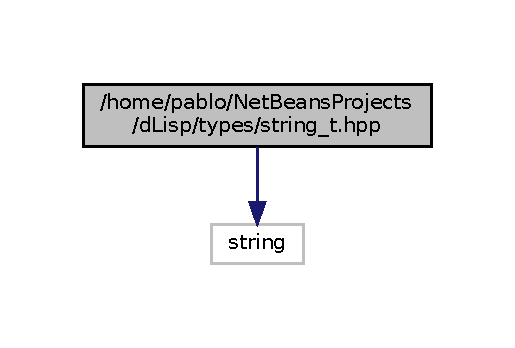
\includegraphics[width=247pt]{string__t_8hpp__incl}
\end{center}
\end{figure}
Граф файлов, в которые включается этот файл\+:
\nopagebreak
\begin{figure}[H]
\begin{center}
\leavevmode
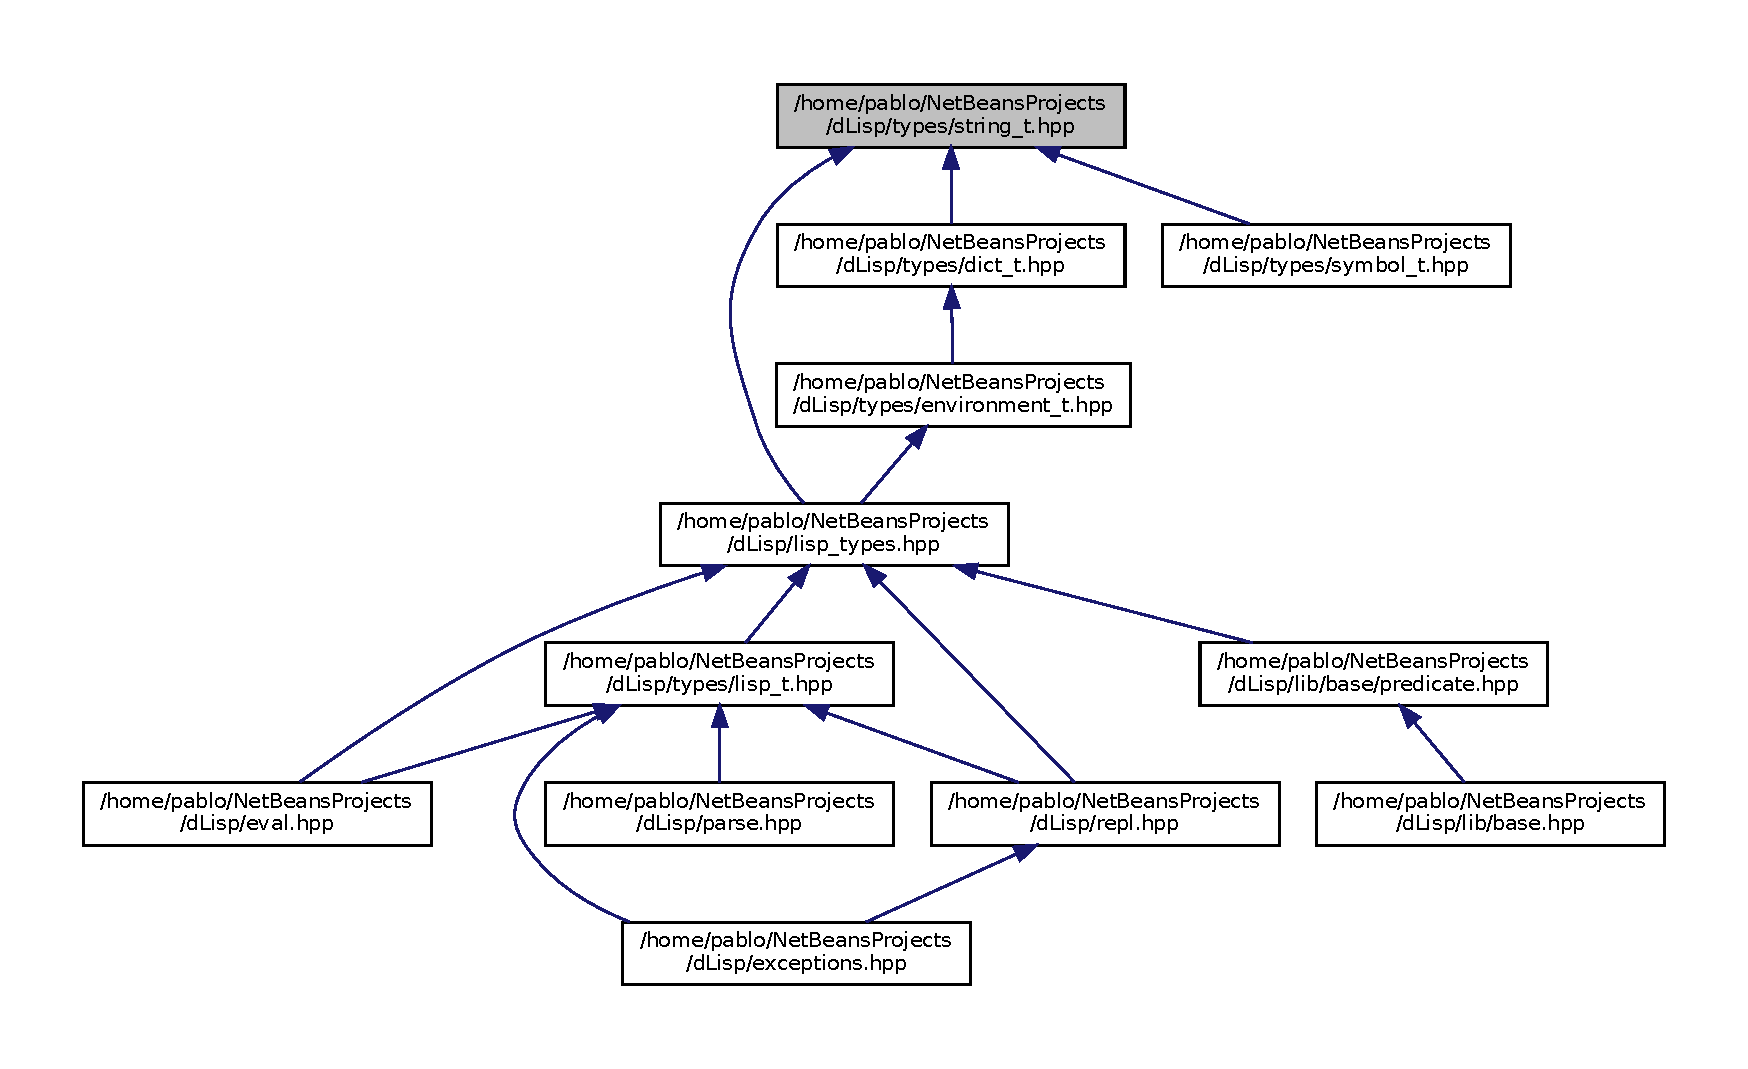
\includegraphics[width=350pt]{string__t_8hpp__dep__incl}
\end{center}
\end{figure}
\subsection*{Классы}
\begin{DoxyCompactItemize}
\item 
class \mbox{\hyperlink{classstring__t}{string\+\_\+t}}
\begin{DoxyCompactList}\small\item\em Класс lisp-\/типа строк \end{DoxyCompactList}\end{DoxyCompactItemize}


\subsection{Подробное описание}
\begin{DoxyAuthor}{Автор}
\+: Павел Коваленко 
\end{DoxyAuthor}
\begin{DoxyDate}{Дата}
23 июля 2018 г., 22\+:25 
\end{DoxyDate}

%--- End generated contents ---

% Index
\backmatter
\newpage
\phantomsection
\clearemptydoublepage
\addcontentsline{toc}{chapter}{Алфавитный указатель}
\printindex

\end{document}
